%Replace Strings:
%PROJECT.TITLE
%TODO.CHANGE
%PROJECT.ABSTRACT.KEYWORDS

\documentclass[12pt, a4paper, oneside]{article}

\usepackage[utf8]{inputenc}
\usepackage[bindingoffset=1.57cm, left=2.54cm, right=2.54cm, top=2.54cm, bottom=2.54cm]{geometry}
\usepackage{mathptmx}
\usepackage{fancyhdr}
\usepackage{lipsum}
\usepackage{secdot}
\usepackage{lastpage}
\usepackage{cite}
\usepackage{tabularx}
\usepackage{booktabs}
\usepackage{graphicx}
	\graphicspath{ {images/} }
	
\usepackage{subcaption}
\usepackage{multirow}

\usepackage{listings}
\usepackage{tocloft}
\usepackage[table,xcdraw]{xcolor}
\usepackage{floatrow}
\floatsetup[table]{capposition=top}

\usepackage{ltxtable}

\linespread{1.2}
\pagestyle{fancy}
\fancyhf{} % sets both header and footer to nothing
\renewcommand{\headrulewidth}{0pt}
\rhead{ \textit{Treasure Nepal: Discover Places, Collect Treasures}}
\cfoot{\thepage}

\setlength{\parindent}{0pt}
\setlength{\parskip}{12pt}

\begin{document}



\pagenumbering{roman}
\large
\begin{center}
	\textbf{ACKNOWLEDGEMENT}
\end{center}

\normalsize

This project would not have been possible without the joint efforts of the college, the teachers, the supervisor and the faculty members. It has been a pleasure for us to acknowledge the assistance and contributions that were very important and supportive throughout the project.

We are highly indebted to our Project Supervisor Er. Madan Kadariya, Head of Department of IT Engineering for his valuable guidance throughout the project development period and for providing technical support with suggestions which helped our project to grow and foster to a certain level we didn’t think of reaching in such a short period. We are also thankful to all the faculty members of Computer Engineering department for providing us with adequate resources and guidance for us to work on this project.

Last, but not the least, we would like to thank our teachers, parents and colleagues who have been knowingly or unknowingly the part of this project and lent support and views during the entire development time.

\break





\addcontentsline{toc}{section}{Abstract}
\large
\begin{center}
	\textbf{ABSTRACT}
\end{center}
\normalsize
As we are at the brim of the Visit Nepal year 2020, the decentralization of tourism in Nepal has become absolutely necessary. Almost ninety percent of the tourists arriving Nepal visit the most popular destinations like Kathmandu, Pokhara, Chitwan and Everest, whereas the remote places like Rara Lake and Phoksundo National Park have not seen satisfactory inflow of tourists despite them being rich in natural beauty and tourism potentiality. There are still a lot of tourist destinations in Nepal that need the attention of the tourists.

Treasure Nepal is a treasure hunt application available in both Android and iOS platforms, where the users travel to different places in order to collect treasures and increase their scores. The app has an integrated map that navigate the users to various tourist destinations in Nepal. The project aims to take the attention of tourists and visitors towards otherwise unnoticed tourists destinations in Nepal. The tourists need to physically reach to a place in order to collect treasures. The tourists who collect treasures at places that are remote and left behind will get higher scores than the ones who visit common popular destinations. The users can compete to get their profiles on top of leaderboard on the basis of the scores they have collected. Moreover, the scores collected by the users will provide them with exclusive offers and discounts on hotels, restaurants, travel agencies, movie tickets, and many more commercial services. On the long run, the project sets its objective to strive for the decentralization of tourists visiting Nepal.

\textbf{Keywords}: Visit Nepal 2020, Treasure hunt, Tourism\\

\break







\large
\addcontentsline{toc}{section}{Table of Contents}
\begin{center}
	\textbf{TABLE OF CONTENTS}
\end{center}
\normalsize
\setlength{\cftbeforetoctitleskip}{0pt}
\renewcommand{\contentsname}{}
\tableofcontents

\break










\large
\addcontentsline{toc}{section}{List of Figures}
\begin{center}
	\textbf{LIST OF FIGURES}
\end{center}
\renewcommand{\listfigurename}{}
\listoffigures

\break










\large
\addcontentsline{toc}{section}{List of Tables}
\begin{center}
	\textbf{LIST OF TABLES}
\end{center}
\renewcommand{\listtablename}{}
\listoftables

\break












\large
\addcontentsline{toc}{section}{List of Abbreviations}
\begin{center}
	\textbf{LIST OF ABBREVIATIONS}
\end{center}

\renewcommand{\arraystretch}{1.2}
\begin{table}[H]
\begin{tabular}{ll}

API & Application Programming Interface\\
CRUD	& Create, Read, Update, Delete\\
CSS		& Cascading Style Sheets\\
DBMS	& Database Management System\\
GDP		& Gross Domestic Product\\
GPS		& Global Positioning System\\
HTML	& Hyper-Text Markup Language\\
HTTP	& Hyper-Text Transfer Protocol\\
IDE		& Integrated Development Environment\\
iOS		& iPhone Operating System\\
JSON &	JavaScript Object Notation\\
LaTeX	& Lamport TeX\\
MVC		& Model View Controller\\
MVP		& Minimal Viable Product\\
NGO		& Non Governmental Organization\\
NHS		& National Health Service\\
NTB		& Nepal Tourism Board\\
QR		& Quick Response\\
RDBMS	& Relational Database Management System\\
REST	& Representational State Transfer\\
SDK		& Software Development Kit\\
SQL		& Structured Query Language\\
SRS		& System Requirements Specification\\
SSD		& System Sequence Diagram\\
UI		& User Interface\\
UML		& Unified Modeling Language\\
URL		& Universal Resource Locator\\
VNY		& Visit Nepal Year\\
XML		& Extensible Markup Language\\
\end{tabular}
\end{table}


\break

%\mainmatter
\cfoot{\textbf{\thepage} /  \pageref{LastPage}}
\normalsize
\pagenumbering{arabic}
\section{Introduction} 
Treasure Nepal is an Android / iOS application for a treasure hunt game targeted to internal as well as external tourists visiting several destinations within Nepal. With the view of encouraging tourists to visit remote and unexplored part of the country, the application aims to increase the traffic of tourist in such remote and unnoticed locations as well as promote their tourism. 

According to Nepal Rastra Bank, the total contribution of the foreign exchange from tourism to the total Gross Domestic Product (GDP) of Nepal was only 2.2\% in the year 2017/18. \cite{tourismstats}. Observing at the statistics, the ratio of contribution of tourism to GDP is not satisfactory in Nepal. Looking at the Federal Budget of Nepal of fiscal year 2019/20,  only Rs. 2.68 billion out of total Rs. 1.53 trillion budget (0.17\%) has been allocated for the development of tourism infrastructures \cite{budget}. This also shows that tourism sector is not getting quite satisfactory budget for its development. For a geographically challenged landlocked country like Nepal, tourism can in fact become one of the major backbones of economy of the nation. For developing the tourism sector in future days, collaboration from all parties -- from government to the common people --- has become absolutely necessary. 

The Government of Nepal has taken efforts to celebrate the year 2020 officially as the Visit Nepal Year 2020. The Government aims to bring two million tourists in Nepal during the year 2020 \cite{visitnepal}. At the brim of year 2020, tourism in Nepal is largely centralized to a few popular destinations. The places like Kathmandu, Pokhara, Chitwan, Annapurna area and Everest area are largely flocked by tourists while destinations like Rara Lake, Shey Phoksundo National Park or Khaptad National park struggle to get satisfactory inflow of traffic. This project is an endeavor taken to contribute as much as we collective can to uniformly distribute the traffic of tourists in different places, to the success of upcoming Visit Nepal 2020 project and tourism development in Nepal as a whole.

\subsection{Project Overview}
Treasure Nepal is an installable mobile application available in both Android and iOS platforms. Once the user installs app and registers her account, she can view various local as well as distant treasures in a map within the application. Each of the treasures have some specified number of points associated with them. When the user decides to collect a treasure, she should physically go to the location where the treasure is installed, and then scan QR code installed at that location. Once the user scans the QR at the treasure location, those points will be awarded to the user's account. The user cannot collect the same treasure again and again. When user's point crosses a certain level, she is provided with several offers, rewards and discounts at various hospitality service providers, preferably the ones that are the nearest.

\subsection{Problem Statement}
The centralization of traffic of tourists visiting Nepal has largely underestimated the potential and beauty of many travel destinations, specially in remote areas. As a result, these places have very low traffic of tourists. In addition, as majority of people in such places rely solely on tourism industry for their livelihood, this problem has pushed those communities even further down below the poverty line. Furthermore, the tourists visiting different places in Nepal may not get sufficient information about the local attractions that are not briefed to them by their guides/agencies. An approach to reliably provide them information about the unnoticed and unvisited places in Nepal, and to encourage them going to that place has been absolutely necessary.

\subsection{Objectives}
The project has put forward the following objectives:

\begin{itemize}
	\item To provide as the deliverables an Android as well as iOS app freely to the users as a means of information about places as well as a method of entertainment.
	\item To decentralize the tourism traffic and encourage uniform flow of tourists at various destinations across Nepal.
	\item To promote and encourage the tourism in remote, unnoticed and novel destinations which otherwise are not popular or have low inflow of tourists.
	\item To promote local businesses and people's life standard in remote places by encouraging the tourists to visit those places.
\end{itemize}

\subsection{Significance of the Study}
The study of this project is significant owing to the fact that the solution to the problem we are trying to solve has rarely been ever created, and our idea is one of the first of its kind. Our approach of trying to solve the problem while providing entertainment to the users will certainly be a reason why people won't hesitate to install and use our application. Also, we are very near to the Visit Nepal Year 2020, and this study will certainly be helpful in some ways in contributing to achieving the objectives set by the Government of Nepal in the year 2020. It is expected that the project will reach to a significant majority of tourists that visit Nepal in 2020, because the inflow traffic of tourists in that year is expected to be higher than usual..

\subsection{Scope and Limitations}
In the current scope, the treasure hunt and reward collection concept of the app are implemented and other features are proposed to be added later in future recommendations. Such possible extensions could be addition of forex plugins, itinerary maps, guides, etc. The users will be able to collect coins from collecting the treasures, and their collection will be put in the leaderboards based on the user's local location as well as country-wise and globally. The application has an integrated map, which enlists the tourist destinations in the locality of tourist's current location. The application is also be connected to third party social networking platforms like Facebook, Twitter, etc. so that the users can login via them. 

The scores of the treasures is be calculated based on the factors like the difficulty to reach the destination, its novelty, potentiality to attract new tourists and other similar criteria. The users will receive more amount of score when visiting rural and novel places than visiting urban and frequently visited places.

The following are the limitations of the project that are realized:
\begin{itemize}
 	\item The application will be built on Android and iOS platform, but not for other mobile operating systems like Blackberry and Windows.
	\item QR code scanning will be the method of collection of treasures and no other validation architecture will be used except for the check of location when the user scans the QR.
 \end{itemize}













\break
\section{Literature Review}
This section consists description of the literature study performed during the development of this project.

\subsection{Visit Nepal 2020}
The Visit Nepal Year (VNY) 2020 project was officially introduced by Nepal Tourism Board (NTB) in 2015 and aims to bring two million tourists in Nepal during the year 2020 \cite{visitnepal}. The year 2020 has been chosen as the national tourism year after the last similar tourism year in 2011. Its slogan -- 'Lifetime Experiences' --  has been translated to more than ten different languages. The tourism board also had developed a plan to train ten thousand people to provide quality service to the tourists. The three major commitments made by the VNY2020 for sustainability are 'Climate Change', 'Community Based Tourism' and 'Going Green' respectively \cite{vny}.

Community based tourism has been very popular in recent years in Nepal, especially in the Himalayan region and along the trekking routes. For instance, the numbers of registered home-stays in Nepal increased from 283 in 2017 to 324 in 2018 \cite{tourismstats}. This number was just 217 in 2015. This increasing interest in the community based tourism is in fact due to the tourist's wish to see the actual lifestyle and living standard of the people living in various communities in Nepal. These forms of tourism not only provide unforgettable experiences to the visiting tourists, but are also a means of income and living for people in such areas. This project has also taken steps to actually promote such local and community based tourism in various places in Nepal.

\subsection{Tourism in Nepal}
Tourism is one of the most important service industry contributing to the economy of Nepal. Being rich in natural, cultural and bio-diversity, Nepal comes within the short list of the budget-friendly choices of tourism destinations all around the world. As the country has finally gained stability after a decade long armed-chaos, political instability and the devastating earthquake, the number of tourists interested to visit Nepal is increasing day by day. As of 2019, the average cost per day of traveling to Nepal is only \$25, which is the reason Nepal has been seen as budget-friendly tourist destination \cite{nepaltravelcost}.

The major itineraries of the tourists visiting Nepal include mountaineering, trekking, religious pilgrimages and holiday spending. The northern part of Nepal has the mountain range with highest elevation in the world, called as the Himalayas \cite{himalayas}. These mountains serve as a destination for the tourists seeking mountaineering as well as trekking. The famous trekking destinations in Nepal are Everest Base Camp, Annapurna Circuit and Langtang Trekking Route \cite{trekkingroutes}. Other attractions include various lakes, the famous of which are Tilicho Lake, Rara Lake, Phewa Lake and Gosaikunda.

Nepal is also rich in biodiversity. Currently there are 12 national parks, 1 wildlife reserve, 6 conservation areas, 1 hunting reserve and 10 Ramsar sites as the protected areas of Nepal \cite{protectedareas}. Among them, Chitawan National Park is the most popular one. A lot of tourists visit these areas for the purpose of jungle safari and animal sports.

Nepal is quite rich in cultural diversity too. Some of the major ethnic groups in Nepal are Kshetri, Brahmins, Magar, Tharu, Tamang, Newar, Kami, Musalman, Yadav, Rai, Gurung, Thakuri, Limbu, etc. A large portion of the tourist inflow in Nepal, especially from south -east Asian countries like India, Bhutan, Thailand, Myanmar, etc. occurs for religious and pilgrimage purposes. In recent years, the various communities have incorporated home stay programme to host tourists in their home and offer their cultural courtesy, which has sent setup good environment for the cultural tourism in Nepal. The festivals like Dashain, Lhosar, Chhath, Gai Jatra, Buddha Jayanti, etc. are some of the most popular festivals of Nepal.

\subsection{Hospitality Industry in Nepal}
Hospitality industry is a collection of service based industries that are focused on providing hospitality services to the consumers. The industries like hotels, lodges, restaurants, food and drink services, event planning services, amusements, adventures, travel and transportation services etc. all come under the common umbrella of hospitality industry. The industry of hospitality is specially important to be studied for this project, because it is those service providers that will provide offers and discounts to the tourists who use the application.

The hospitality industry is largely operated by private and Non Governmental Organization (NGO) sectors in Nepal. Some of the major businesses in the field of tourism in Nepal are hotels, restaurants, lodges, travel agencies, ticket providers, tour guides, rafting agencies, mountaineering agencies, trekking agencies, recreational aviation, etc. Some statistics on number of different businesses providing hospitality services are listed in Table \ref{table:tourismindustry}.

\renewcommand{\arraystretch}{1.5}
\begin{table}[H]
\begin{tabularx}{\linewidth}{|c|X|c|}
\hline
\rowcolor[HTML]{C0C0C0} 
\textbf{S.N.}                & \textbf{Description} & \textbf{Number}   \\ \hline
1.  & Star Hotels     & 129                          \\ \hline
2.  & Tourist Standard Hotels    & 1125       \\ \hline
3.      & Total Hotels   & 1254          \\ \hline
4. & Travel Agencies    & 3508 \\ \hline
5. & Trekking Agencies & 2649            \\ \hline
6.  & Rafting Agencies    & 73          \\ \hline
7.      & Tourist Transportation Services  & 77      \\ \hline
\end{tabularx}
\footnotesize Source: Tourism Statistics, 2018. Ministry of Culture, Tourism and Civil Aviation. \cite{tourismstats}
\caption{Tourism Industry Statistics in Nepal in Year 2075 BS}
\label{table:tourismindustry}
\end{table}

%
%\subsection{Related Laws and Legislations}
%The Ministry of Culture, Tourism and Civil Aviation (MoCTCA) is the authoritative body of the Government of Nepal that looks upon the sector of tourism in Nepal. The ministry has a separate department named Department of Tourism for this purpose. The Government of Nepal in a joint partnership with private sectors in tourism have established Nepal Tourism Board (NTB) in 1998 by Parliament of Nepal with an act named Nepal Tourism Board Act 1997 to develop and market Nepal as a beautiful tourism destination \cite{ntbact}. At present, Nepal Tourism Board works actively in collaboration with Ministry of Culture Tourism and Civil Aviation to conduct various events and activities to promote tourism sector in Nepal.
%
%Table \ref{table:tourismlaws} enlists some of the major laws and regulations that are currently enforced in the tourism industry in Nepal. If this project is to be taken to production level, it should be registered to Nepal Tourism Board and the permission of MoCTCA is required to start providing services to the consumer base. As per Section 3 of Nepal Tourism Board Rules 1999, a tourism entrepreneur should pay a service fee of two percent over the total amount paid each tourist \cite{ntbrules}. In the current scope, the points collected in this application will not have direct monetary value and cannot be exchanged with cash. If the project is expanded and taken to the level where users will be able to use the points just as cash in virtual form, then a consent as well as permission from Nepal Rastra Bank is required.
%
%\renewcommand{\arraystretch}{1.5}
%\begin{table}[H]
%\begin{tabularx}{\linewidth}{|c|X|c|}
%\hline
%\rowcolor[HTML]{C0C0C0} 
%\textbf{S.N.}                & \textbf{Act / Rule / Law} & \textbf{Year (AD)}   \\ \hline
%1.  & Tourism Act     & 1978                          \\ \hline
%2.  & Tourism Policy    & 2008       \\ \hline
%3.      & Travel and Trekking Agency Rules  & 2005          \\ \hline
%4. & Hotel, Lodge, Restaurant, Bar and Tourist Guide Rules    & 1981 \\ \hline
%5. & Mountaineering Expedition Rules & 2002            \\ \hline
%6. & Nepal Tourism Board Act & 1997 \\ \hline
%7.      & Nepal Tourism Board Rules & 1999      \\ \hline
%\end{tabularx}
%\footnotesize Source: Government of Nepal : Ministry of Culture, Tourism and Civil Aviation. \cite{tourismacts}
%\caption{Some acts and laws related to the project and tourism sector}
%\label{table:tourismlaws}
%\end{table}

\subsection{Cross Platform App Development}
Any application that is developed targeting both of these platforms is known as a cross platform application. Android and iOS are two major mobile development platforms in the market today. In today's market, the businesses have opted to allow all of their users use their services through all of the technological platforms available to the client. For example, the same services of a company can be used by a web based portal, an Android mobile phone, an iPhone, iPad, or even a desktop computer software.

When the matter comes to cross-platform mobile application development, the most popular frameworks available today are Flutter, Ionic and React Native \cite{rnvsflutter}. The two frameworks are compared in Table \ref{table:rnvsflutter}. React Native is relatively older technology first released in 2013 and currently managed by Facebook Inc. Flutter, a new technology, is the similar framework from Google. React Native uses JavaScript as its language while Flutter uses Dart. So, to use Flutter, one has to learn Dart first, which itself is not a primary language many developers learn in early stages of their programming career. React Native being older has relatively wider support and user base than flutter. Flutter is rapidly increasing its user base too. The choice between one of them depends upon the programmer's preferences and choices. We opted to use React Native in stead of Flutter in this project because of the team member's pre-familiarity with Javascript language and better community support. 


\renewcommand{\arraystretch}{1.5}
\begin{table}[H]
\begin{tabularx}{\linewidth}{|c|c|X|X|X|}
\hline
\rowcolor[HTML]{C0C0C0} 
\textbf{S.N.}                & \textbf{Category} & \textbf{React Native} & \textbf{Ionic} & \textbf{Fluttter}   \\ \hline
1. & Developed By    & Facebook and Community  & Drifty Co. & Google and Community     \\ \hline
2. & Released   & 2013 (Open Sourced in 2015)  & 2013 & 2017     \\ \hline
3. & Language    & JavaScript  & HTML, CSS, JavaScript & Dart     \\ \hline
4. & Community Support  & Old and Strong  & Old and Strong & Relatively new     \\ \hline
5. & Used By   & Facebook, Instagram, Tesla, Uber, Walmart, Airbnb  & Marketwatch, NHS, SWorkit, Untapped & Alibaba, Google Ads, Tencent     \\ \hline
\end{tabularx}
\footnotesize Source: CodeBurst.io \cite{rnvsflutter}
\caption{Comparison between React Native, Ionic and Flutter}
\label{table:rnvsflutter}
\end{table}


\subsection{Client Server Architecture}
Client-Server architecture is a model of computing where the services and resources to be provided are managed by a computer called a server and the provided services are utilized and used in the computer called a client, as shown in Figure \ref{fig:clientserver}. The clients use the services hosted by the server with the use of a network or internet connection. There are several noticeable advantages of using a client server architecture in stead of a single tier architecture. The most important of them is the separation of workloads between the two computers. The maintenance also becomes easy as all the services and resources are hosted by a single computer. The separation of the client and server enables the developers to employ security strategies in both client and server layer and thus makes it more secure. Data and resource sharing is also improved by the use of a central server where all the clients can have access to.

In our project, the server tier is the API server that will handle all the data requests received from mobile device and the client will the application running in Android phone or iPhone.

\begin{figure}[H]
	
\includegraphics[width=\linewidth]{client-server.png}
	\centering
	\caption{Client Server Architecture}
	\label{fig:clientsever}
\end{figure}


\subsection{REST API}
API stands for Application Programming Interface. It is a set of of functions, procedures and protocols between a client and a server so that the client can use the application and services of a server. An API can be Web Service based, Operating System based or Database Management System (DBMS) based. Web based APIs are those which provide the interface between the client (Presentation logic) and the database (data and business logic). A client can initiate either a read or a write operation request the API server on some data. Each time a client sends a request to the API server, it breaks it down to different database operations and then read/write data to the database. The API server also sends back the data it receives from the database in formats like XML(Extensive Markup Language) or JSON(JavaScript Object Notation).

REST stands for Representational State Transfer. It is a software architecture that defines a set of constraints for creation of web services and APIs. The web services that abide by these constraints are commonly called RESTful. The web services are the programs that are run in the server that respond to various HTTP requests like GET, PUT, POST, DELETE, etc. and send response to the client of those services.

Hence, a RESTful API is defined as a software architecture where an API server provides its clients with various endpoints through which the client can read and write data from/to the database. The API server is programmed in such a way that it returns a specific set of dynamic data when one of it's endpoint is hit with correct method, authentication header, body and parameters. Table \ref{table:apiconventions} shows commonly used convention in request-response model of a RESTful API.

\begin{table}[H]
\begin{tabularx}{\linewidth}{|c|c|c|c|X|}
\hline
\rowcolor[HTML]{C0C0C0} 
URL              & Method & Parameters &  Body & Commonly Used For                                                                              \\ \hline
/endpoint/       & GET    &                                   &                             & Get all entries from the database                                                              \\ \hline
/endpoint/\{id\} & GET    &                                   &                             & Get the entry corresponding to the provided id                                                 \\ \hline
/endpoint/       & GET    & params                            &                             & Get a list of entries that are filtered by provided parameters                                 \\ \hline
/endpoint/       & POST   &                                   & entry                       & Add the new entry into the database                                                            \\ \hline
/endpoint/\{id\} & DELETE &                                   &                             & Delete the entry corresponding to the provided id                                              \\ \hline
/endpoint/\{id\} & PUT    &                                   & new\_entry                  & Update the entry corresponding to the given id with new entry                                  \\ \hline
/endpoint/\{id\} & PATCH  &                                   & \{attr: value\}             & Update only the specified attributes of the entry corresponding to provided id with new values \\ \hline
\end{tabularx}
\caption{Commonly used convention in API Programming}
\label{table:apiconvention}
\end{table}

\subsection{JavaScript Object Notation}
JavaScript Object Notation (JSON) is an open-standard lightweight method of data interchange. It is one of the widely used method of exchange of data between client and server in RESTful API architecture. JSON makes use of key-value pairs of strings to represent data. The collection of unique keys and corresponding values is known as JSON object. A collection of JSON objects is known as a JSON array. A JSON object is enclosed in curly braces '\{ \}' whereas the JSON array is enclosed inside square brackets '[ ]'. In Figure \ref{fig:json}, an example of JSON array consisting of two JSON objects is shown.


\begin{figure}[H]
	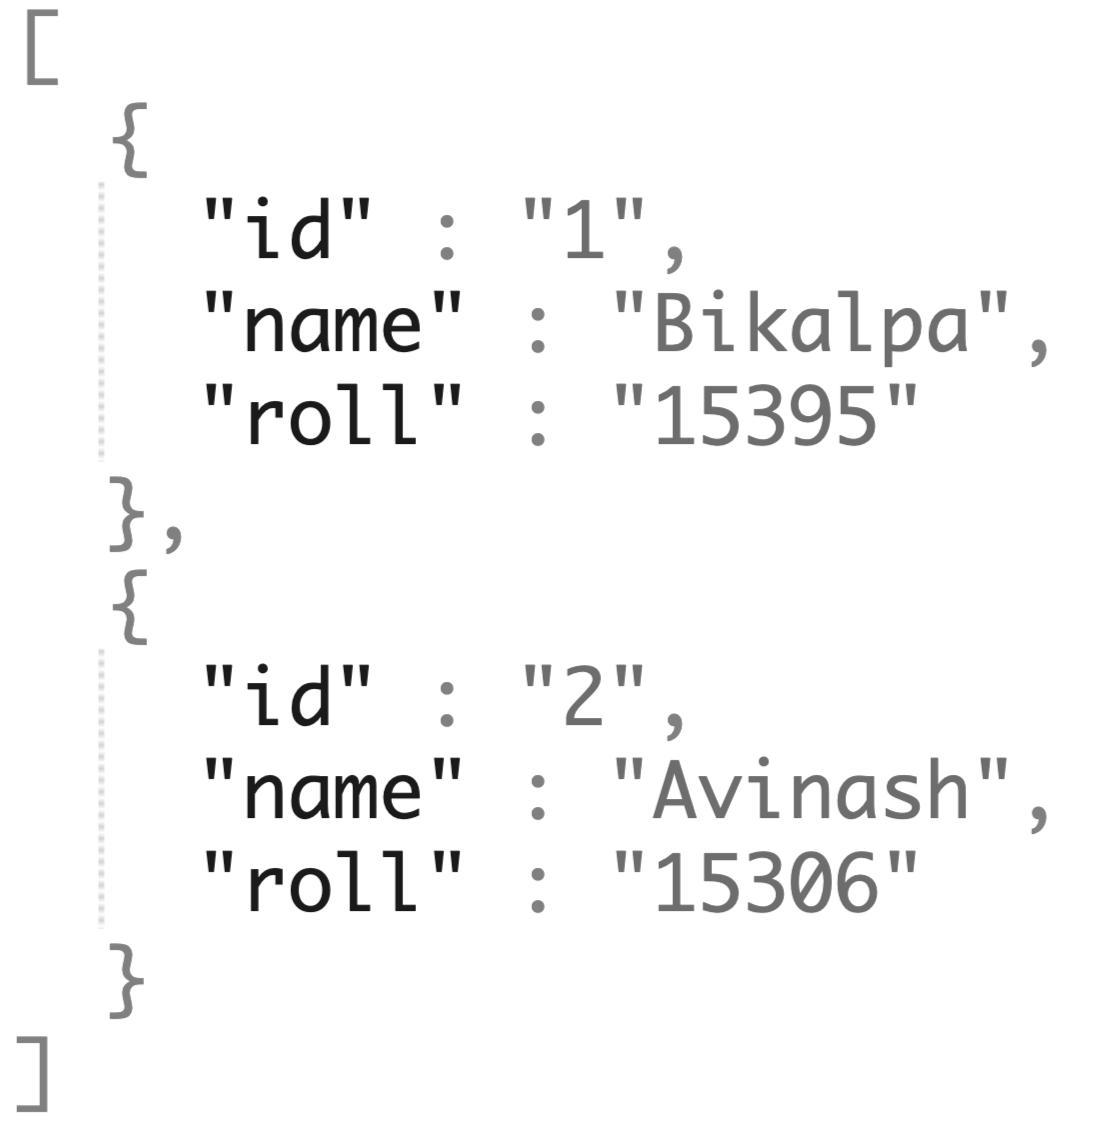
\includegraphics[width=0.3\linewidth]{json.png}
	\centering
	\caption{The format of JSON object and array}
	\label{fig:json}
\end{figure}

It is quite important to note the difference between an actual JavaScript Object and a JSON formatted object. The first and foremost difference is that JSON is just a format of transferring text, that just happens to be formatted in a way JavaScript objects are written. The JSON object doesn't directly correspond to a JavaScript object. In fact, JSON only supports strings as its key and value, whereas the values in JavaScript object can be any data type. A parser is needed to first convert a JSON string to actual JavaScript object if it is to be used inside JavaScript code.

\subsection{Global Positioning System}
Global Positioning System, also abbreviated as GPS is a global system of satellite based navigation where about a total of 33 satellites orbit the earth to provide geolocation and time information to the receiver anywhere in the earth. As of 2019, the GPS is owned by the United States Government and operated by United States Air Force \cite{gps}. It is freely available for use to everyone with the use of a GPS receiver. Today, almost all of the smartphones have a built-in GPS sensor which they use as the method of navigation.

The GPS satellites any particular time, a GPS receiver is directly in line-of-sight with at least four satellites. All of the 33 GPS satellites regularly emit radio waves carrying information about their current position and time. When a GPS receiver receives those radio waves, it can figure out how far away from those satellites it currently is. Based on the distance of the GPS receiver from at least three satellites in its line of sight, the receiver can deduce its location by the method called as trilateration \cite{gps}.

Let us consider a GPS receiver that is in line of sight to three GPS satellites at some place in the world. When the receiver figures out its distance from one of the satellites, its actual position is somewhere in the surface of the sphere centered at the position of satellite, with radius equal to the distance from the satellite. If the receiver knows its distance from all of three satellites, its position is exactly at the intersection of three spheres centered at each of the satellites with radius equal to the distance between them and the receiver, as shown in Figure \ref{fig:trilateration}. In this way, the accuracy of the position of receiver can be pin-pointed to the accuracy of about 30 centimeters \cite{gps}.

\begin{figure}[H]
	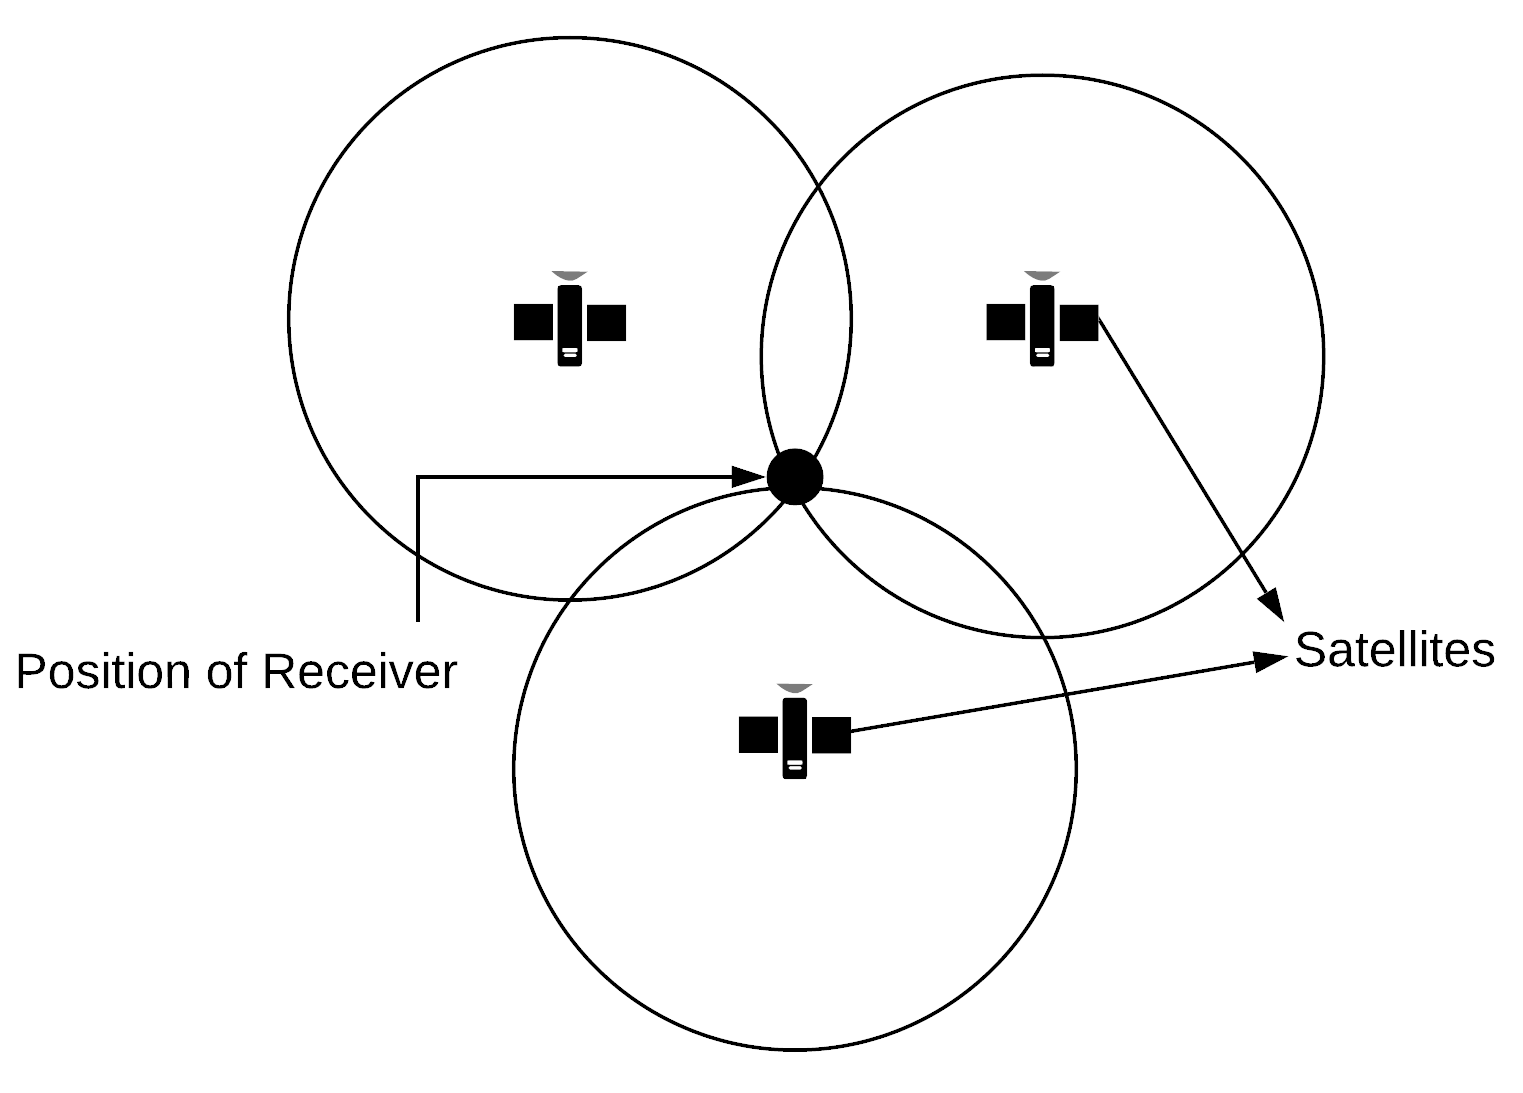
\includegraphics[width=0.5\linewidth]{trilateration.png}
	\centering
	\caption{Identification of geolocation by trilateration}
	\label{fig:trilateration}
\end{figure}

\subsection{Longitude and Latitude} \label{latlng}
The position of any point in the world can be precisely described by two real numbers called longitude and latitude. To make this possible, 180 equidistant and parallel horizontal imaginary lines are drawn over the surface of the earth, which are called latitudes. The longitudes, also called as meridians are the 360 vertical lines that have their ends at the two poles of the earth and span through the surface of the earth. As a reference, the longitude that passes through the center of the earth , also called the equator, is considered as 0 degrees latitude. In the similar way, the longitude line that passes through the British Royal Observatory in Greenwich England is considered as 0 degrees longitude. The distance between two consecutive latitude or longitude is considered as one degree. As a convention, the northern hemisphere is counted as positive latitude and the southern hemisphere as negative latitude. Similarly, the the hemisphere to the east of 0 degree is considered positive and the western hemisphere is considered to have negative longitude. To precisely locate a point in the earth, we provide a coordinates of two real numbers, which describe the distance of the point in degrees from the 0 degree latitude and 0 degree longitude lines respectively.

Given the coordinates of two points, we need to find the distance between those two points on the surface of the earth when we have to verify whether the tourist collected the treasure from within a permitted area around the actual treasure location or not. This distance between the two points on the surface of earth, also called as the great-circle distance can be calculated by using Haversine Formula \cite{haversine}.

Let us consider two points $A$ and $B$ on the surface of the earth with co-ordinates $(\psi_1, \phi_1)$ and $(\psi_2, \phi_2)$. Let $R$ be the radius of the earth. Then according to the Haversine Formula, the great-circle distance $d$ between the points $A$ and $B$ can be calculated as:
\begin{equation}
 d = 2R \sin^{-1} \left( \sqrt { \sin^2 \left( \frac{\phi_2 - \phi_1}{2} \right) + \cos{\phi_1} \cos{\phi_2} \sin^2 \left( \frac{\psi_2 - \psi_1}{2} \right) } \right) 
 \label{eq:haversine}
\end{equation}
% + \cos{\phi_1} \cos{\phi_2} \sin^2 \left( \frac{\psi_2 - \psi_1}{2} \right) 

\subsection{Similar Applications}
There are several treasure hunt applications available in the application stores developed for entertainment purposes. Some of them are GooseChase, Locandy, Huntzz, Scavify and Geocaching \cite{similarapps}. This application distinguishes itself from these applications due to its focus on the tourism industry. The available applications are developed only for entertainment purposes. The existing applications are actually used for challenging friend / family to solve some puzzle and collect treasures within a small amount of area. In contrast, our application covers the whole country. Also, the users themselves have to set treasures and spots and enter them into the application to create a challenge and then challenge someone else to find and collect them. In contrast, the users of the proposed application are already provided with the treasures and they don't actively take participation in creating one.

\subsection{Challenges}
One of the major challenges realized is the validation of the collection of treasures by the users. If only QR code is used for validating that a tourist has in fact reached a destination, there is a high chance that the QR codes get shared among people and people will remotely validate themselves having gone to a place and collected a treasure just by scanning the photo of the QR from a remote location. A countermeasure that can be used is to add actual location data from the user's phone's GPS sensor as an additional parameter for validation. A treasure is only considered to be collected if a user scans the QR from within a specific distance from the actual treasure location. That distance can be calculated using the Haversine formula discussed in section \ref{latlng}.

GPS spoofing is one of the major challenges for any system that has used GPS for the validation. GPS spoofing is the process of modifying a GPS receiver unit so that it broadcasts incorrect GPS signal. The solution to GPS spoofing problem is quite complex and out of scope right now. However, some countermeasures to tackle GPS spoofing are monitoring absolute as well as relative GPS signal strength; checking time intervals and performing comparison; and performing sanity checks \cite{gpsspoofmeasures}.














\break
\section{Methodology}
This section describes the methodology that have been followed during the development of the project.

\subsection{Software Development Life Cycle}
The project has been developed as per the waterfall model of software development life cycle as depicted in Figure \ref{fig:sdlc}. The reason for choosing this model is the lack of sufficient time duration for agile and iterative methods, as well as very low chances of the changes of requirements in the process of development. 

\begin{figure}[h]
	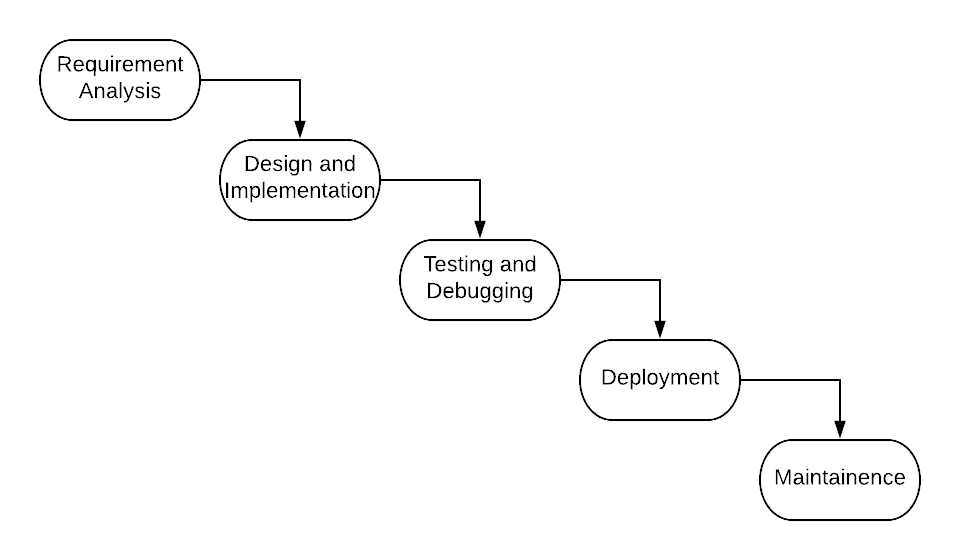
\includegraphics[width=\linewidth]{sdlc}
	\centering
	\caption{Waterfall model of software development life cycle}
	\label{fig:sdlc}
\end{figure}

The life cycle began when the team collected and evaluated the requirements expected from the application. The design and implementation phase was to design and build both API services and client applications. By the end of this phase, a minimal viable product (MVP) was already constructed. In the testing and debugging phases, the quality control methods were be applied to both API and application. Finally, the application was deployed to the local server at the end of the deployment phase. 
%However, there might be slight modifications in the original waterfall model where the design and implementation may be changed slightly after the testing phase if seen reasonable.



\subsection{Technologies Used}
Table \ref{table:tech} consists of the major technologies that are proposed to be used during development and deployment of the application. They are briefly described in the subsections that follow.

\renewcommand{\arraystretch}{1.5}
\begin{table}[H]
\begin{tabular}{|l|l|}
\hline
\rowcolor[HTML]{C0C0C0} 
\textbf{Subject}    & \textbf{Tools and Technologies Used} \\ \hline
Backend Database            & MySQL                        \\ \hline
REST API Service    & Django REST Framework; Postman        \\ \hline
Android Application  & React Native; Android SDK                 \\ \hline
Android / iOS application  & React Native; iOS SDK; XCode              \\ \hline
IDE / Code Editor& Sublime Text; JetBrains WebStorm  \\ \hline
Version Control System& GitHub  \\ \hline
Documentation & LaTeX \\ \hline
\end{tabular}
\caption{Technologies proposed to be used}
\label{table:tech}
\end{table}

\subsubsection{MySQL}
MySQL is one of the most widely used relational database management system (RDBMS). The major reason for us to choose this database is our previous familiarity with the database and it being completely open source. Some of the established tech corporates like Facebook, Twitter, Youtube etc. use MySQL. It also has very good user base and the usage is easier thanks to comprehensive documentation and support.

\subsubsection{Django REST Framework}
Django REST framework is an open source framework for building Web APIs. The framework provides features like authentication, tokenization, session handling, serialization, etc. for users to build API in short amount of time. The programming language used is Python. The reason for choosing this framework is the team members previous familiarity and experience in working with Python programming language.

\subsubsection{Postman}
Postman is an application software that is used for testing API web services. It lets users provide URL, parameters, body and headers to send the request and also shows the response in raw as well as pretty form.

\subsubsection{React Native}
React Native is an open source framework for building mobile applications using Javascript language. In addition to the usage of widely used language like Javascript, it also has cross platform support so that both Android and iOS applications can be built using same code base. Compared to its immediate rival -- Flutter -- it uses relatively easy and familiar language as compared to Dart used by Flutter. We chose this framework due to lack of time to learn Dart language and our familiarity with JavaScript language.

\subsubsection{Android SDK}
Android Software Development Kit is a set of build tools and libraries developed by Google Inc. to let developers develop applications in the Android platform. React Native also uses the Android build tools to eventually compile the application code and install it on the android device.

\subsubsection{iOS SDK}
iOS Software development Kit is a set of libraries and build and debugging tools developed by Apple Inc. to allow developers to develop applications and software in the iOS platform. React Native requires iOS SDK in order to build the compiled iOS application that could run on an iOS device.

\subsubsection{XCode}
XCode is a proprietary Integrated Development Environment (IDE) for macOS, primarily used for developing applications for the iOS and Mac platforms. XCode is frequently required to change native code for asking permissions, interacting with device sensors, installing third party APIs with keys, etc.

\subsubsection{Sublime Text}
Sublime Text is a light-weight cross-platform code editor written in C++ and Python. It is very popular among the developers due to ability of customization and plugins. This editor was chosen for development of backend due to our early experience working on it.

\subsubsection{JetBrains WebStorm}
JetBrains WebStorm is a commercial and proprietary IDE developed by JetBrains for JavaScript development. This IDE was chosen because of it's amazing code completion feature and easier debugging.

\subsubsection{GitHub}
GitHub is a platform for hosting and sharing software development version control by using Git. Github was acquired by American company Microsoft Corporation in 2018. The reason for using this platform was our early experience with it. 

\subsubsection{LaTeX}
LaTeX is widely used documentation preparation system for preparation of scientific documents, books and technical papers. It uses plain text for formatting unlike other document creation systems. The source code is compiled by a compeller to generate the printable/viewable document. The reason for using LaTeX for documentation was to learn this new form of documentation.


\subsection{APIs and Libraries Used}
In course of developing this project, we have integrated several open source as well as proprietary APIs and libraries into our application. Some of the major APIs and libraries used in this project are listed in Table \ref{table:apiandlibrary}.

\begin{table}[H]
\begin{tabularx}{\linewidth}{|c|X|X|X|}
\hline
\rowcolor[HTML]{C0C0C0} 
{\color[HTML]{000000} S.N.} & {\color[HTML]{000000} Name}                                               & {\color[HTML]{000000} Author / Developer} & {\color[HTML]{000000} Used For}                                         \\ \hline
1.                          & \begin{tabular}[c]{@{}l@{}}Google Maps SDK\\ (Android / iOS)\end{tabular} & Google Inc.                                            & Showing Google maps inside our application for users to view treasures. \\ \hline
2.                          & React Native Paper                                                        & Callstack                                              & Material Design UI library for developing Android and iOS application   \\ \hline
3.                          & react-native-maps                                                         & React Native Community                                 & Integration of Google Maps / Apple maps inside of mobile application    \\ \hline
4.                          & react-navigation                                                          & React Navigation                                       & Navigating users from one screen to another inside mobile application   \\ \hline
5.                          & redux                                                                     & Dan Abramov and Andrew Clark                           & State management in mobile application                                  \\ \hline
6.                          & react-native-camera                                                       & React Native Community                                 & Access mobile device's camera and scan QR codes                         \\ \hline
7.                          & react-native-vector-icons                                                 & Joel Arvidsson                                         & Showing vector icons at various places in mobile application            \\ \hline
8.                          & react-redux                                                               & Redux                                                  & Using redux library inside of a React Native application                \\ \hline
9.                          & django-rest-auth                                                              & Tivix                                                  & Authentication inside Django Rest Framework                \\ \hline
\end{tabularx}
\caption{List of APIs and libraries used in the project}
\label{table:apiandlibrary}
\end{table}


\subsection{Method of Data Collection}
Our team has collected data about the various tourist destinations and places (the data include the location, the photos, latitude, longitude, how to get to that place, entry fee, etc.) so that we can add treasures to those places and add them to our database.

In this project, we have used secondary source of data collection. We did not go to those tourist attractions by ourselves but collected the information about them through the use of Internet. The latitude and longitude information were collected by the help of Google Maps, while the address, description, etc were collected from various tourist blogs and websites. As a result, the collected data are not quite reliable and are used only for demo purpose. For more reliability, we can use primary source of information by directly going to thos places and collecting data.

Figure \ref{fig:data-model} shows a sample of data collected by our team.

\begin{figure}[H]
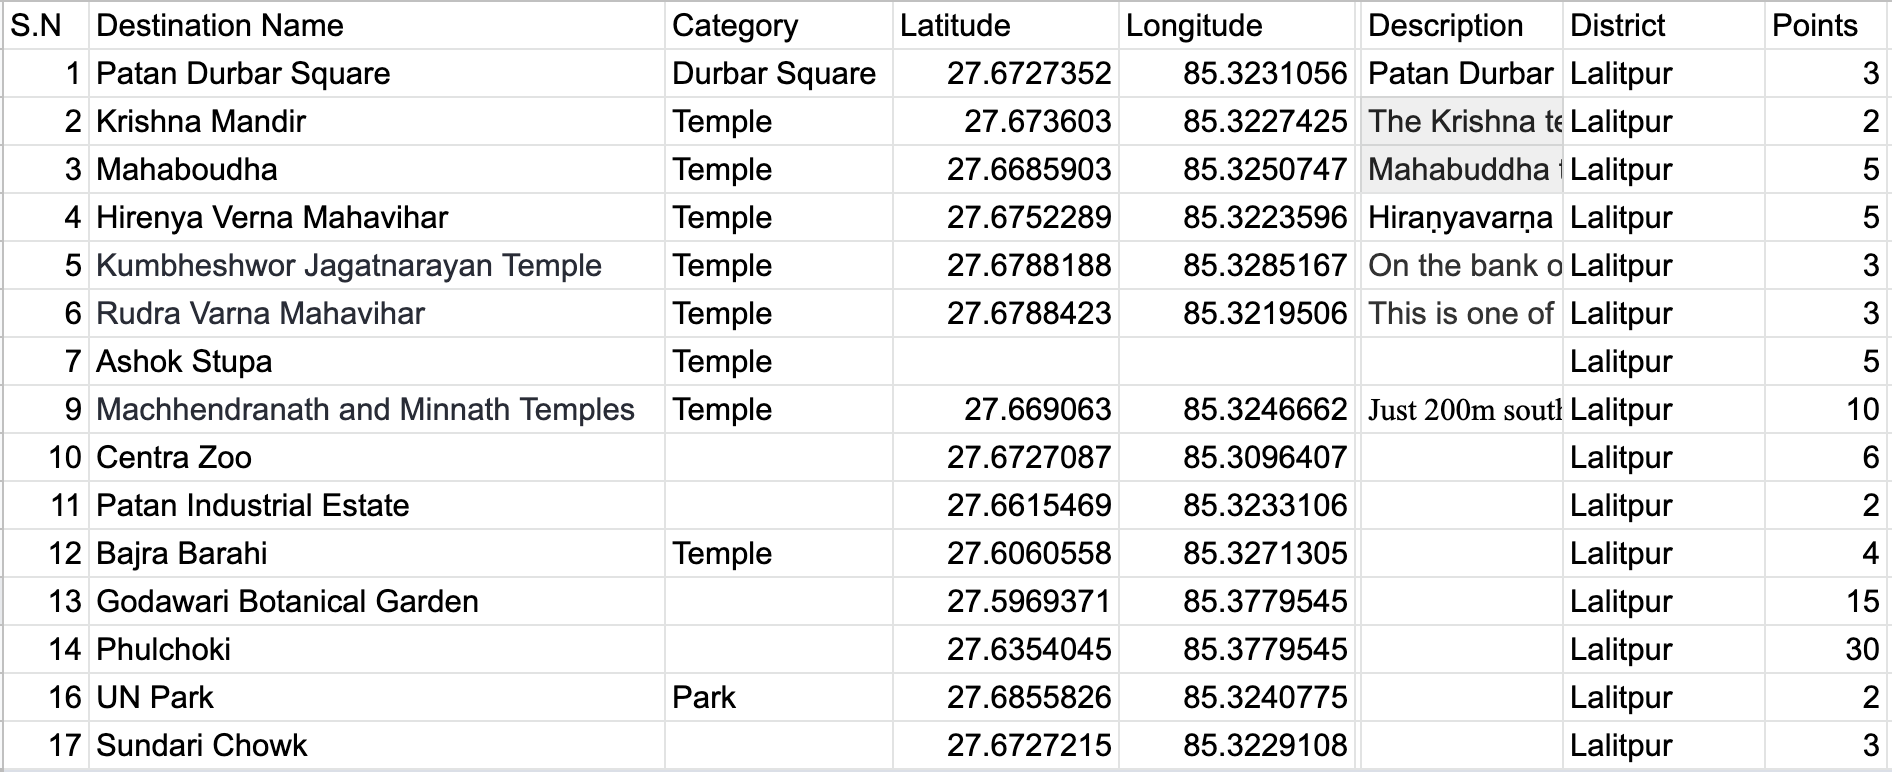
\includegraphics[width=\linewidth, keepaspectratio]{screenshots/data-collection.png}
\centering
\caption{Model of data collection}
\label{fig:data-model}
\end{figure}


\subsection{Team Members and Role Division}
Table \ref{table:team-roles} shows the various roles and responsibilities divided among the team members during the development of this project.

\begin{table}[H]
\begin{tabularx}{\linewidth}{|c|c|p{2cm}|X|}
\hline
\rowcolor[HTML]{C0C0C0} 
S.N.                 & Team Member                        & Role                  & Responsibilities                                                                                                                                                                 \\ \hline
                     &                                    & Requirement Engineer & Collect and analyze various functional and non functional requirements of the project. \newline Prepare System Requirements Specificatiotn (SRS) document                                 \\ \cline{3-4} 
                     &                                    & Systems Designer      & Design high level abstract architecture of the overall project                                                                                                                   \\ \cline{3-4} 
                     &                                    & Data Collection       & Collect data about treasures and rewards to show them in the application                                                                                                         \\ \cline{3-4} 
\multirow{-4}{*}{1.} & \multirow{-4}{*}{Avinash Shreshta} & Backend Developer     & Develop API endpoints to get request from and send response to the mobile application                                                                                            \\ \hline
                     &                                    & Project Manager       & Manage the project team and guide the team along various phases of project development.                                                                                          \\ \cline{3-4} 
                     &                                    & Frontend Developer    & Prepare User Interface of the mobile application. \newline Implement efficient algorithms to cache the data received from API to the local storage                                        \\ \cline{3-4} 
                     &                                    & Backend Developer     & Develop authentication module for a client to authenticate itself to the API server. \newline Design the format of data model exchanged between front end and backend                     \\ \cline{3-4} 
                     &                                    & Document expert  & Prepare final document for submission to the project office.                                                                                                                     \\ \cline{3-4} 
\multirow{-5}{*}{2.} & \multirow{-5}{*}{Bikalpa Dhakal}   & System Tester         & Design different test cases for testing the application. \newline Run various tests to ensure that the final project developed meets the original requirements specified in SRS document. \\ \hline
\end{tabularx}
\caption{Division of roles and responsibilities of team members}
\label{table:team-roles}
\end{table}






\pagebreak
\section{Requirement Analysis}
The requirement analysis of the product to be developed was done before everything else during the project. During this phase, our team worked together to find out what features were expected of the product to be developed. It was also helpful to filter what is important and what is not important features to be added in the application. The requirements were widely categorized into functional and non functional requirements. The process we used during this phase are described in the sections that follow.

% 

%\subsection{Feasibility Study}
%Feasibility study is the assessment of how practicable a proposed project is. For a project to be feasible, it should both be technically as well as economically feasible. For technical feasibility, we studied about to what extent can we use an end user's mobile device to collect data and information needed for the implementation of the project. We found that major sensitive data we receive from the user is the user's location. But looking at every mobile applications that use location services, the use of user's location in our application is not quite infeasible.

\subsection{Requirements Elicitation}
Requirement elicitation is the process of collecting and noting down several types of requirements that are expected of the product from various sources like development team, the consumer, users, experts, etc. Prioritizing the collected requirements is also an important task done in this phase. Elicitation is the first step in developing the requirements documentation in any software project. In this project, the major sources for eliciting the requirements where the team members and the supervisor assigned to the project team.

During requirement elicitation, the team members conducted elicitation meetings with the supervisor to find out and note out requirements from 'absolutely necessary' to 'desirable'. During the process, each of us acted as an end user and described what an end user would expect the product to do. We would then discuss about whether the requirement is necessary or not, whether it is feasible to implement in our project and then note them in neat and tidy way. The team members then categorized the requirement into several categories that are described in the subsections that follow.

\subsubsection{Functional Requirements}
Functional requirements are those requirements which define a system or a component by the functions it should perform. These are the requirements that are absolutely necessary to be in the product. The functional requirements of our project are listed in Table \ref{table:functionalreq}.

\begin{table}[H]
\begin{tabularx}{\linewidth}{|c|X|c|}
\hline
\rowcolor[HTML]{C0C0C0} 
{\color[HTML]{000000} S.N.} & {\color[HTML]{000000} Functional Requirements}                                                                             & {\color[HTML]{000000} Priority} \\ \hline
1.                          & The user should be able to download and install the application in a Android Phone or iPhone                               & Very High                       \\ \hline
2.                          & The user should be able to register his/her account in the application and login at any time with valid credentials        & Very High                       \\ \hline
3.                          & The user should be able to view treasures in a map and get information about the treasures.                                & High                            \\ \hline
4.                          & The user should be able to view rewards that he/she is eligible to collect and read their details.                         & High                            \\ \hline
5.                          & The user should be able to scan a treasure and have the points collected in his/her account.                               & High                            \\ \hline
6.                          & It will be possible to scan a treasure once and only once and only when the user is in vicinity of the treasure's location & Very High                       \\ \hline
7.                          & The points provided to a particular treasure should be practical and dependent on factors like reachability, cost, etc.    & High                            \\ \hline
\end{tabularx}
\caption{List of functional requirements of the project}
\label{table:functionalreq}
\end{table}

\subsubsection{Non-Functional Requirements}
Non functional requirements are those which describe quality attributes in a system. These are the requirements that are not absolutely necessary, but are desirable for good quality of the proposed product. The non-functional requirements of our project are listed in Table \ref{table:nonfuncreq}.

\begin{table}[H]
\begin{tabularx}{\linewidth}{|c|X|c|}
\hline
\rowcolor[HTML]{C0C0C0} 
{\color[HTML]{000000} S.N.} & {\color[HTML]{000000} Non Functional Requirements}                                                                                                      & {\color[HTML]{000000} Desirability} \\ \hline
1.                          & The permitted distance from the location of the treasure up-to which the collection of treasure is allowed could be specified and entered into database & High                                \\ \hline
2.                          & The users should be able to login via email as well as Google and Facebook                                                                              & Medium                              \\ \hline
3.                          & The user will be able to share the application via email or social media to invite other people to play                                                 & High                                \\ \hline
4.                          & The rewards offered to the users could be provided on the basis of user's personal preference.                                                          & Medium                              \\ \hline
5.                          & The application should be user-friendly                                               & High                              \\ \hline
\end{tabularx}
\caption{List of non functional requirements of the project}
\label{table:nonfuncreq}
\end{table}


\subsection{Requirements Specification}
A Software Requirement Specification (SRS) is a detailed description of both functional and and non functional requirements of a software project that are formatted and documented for later reference. The most widely used tools for requirement specification are the use case stories, UML use case diagrams, use case descriptions and UML activity diagrams. During requirement specification, the requirements elicited in earlier phases were further dug into detail and then it was converted to diagrammatic form. 

\subsubsection{User Stories}
In the initial phase of requirement specification, a particular scenario is imagined and then a descriptive story of what the user would experience and expect are prepared from the point of view of the users themselves. These descriptive stories are called user stories.

On the highest level of abstraction, the team members created a scenario where a user has first interacted with the application and how he would use it. The user story in that story is depicted  in Table \ref{table:user-story-use-application}.


\begin{table}[H]
\centering
\begin{tabularx}{\linewidth}{|X|} 
\hline
\textbf{User Story:  Use Application}\\ 
\hline
When the user first installs the app, she should be able to sign up for a new account. For so, the user can either use email address or use Facebook and Google for authentication. Once the user registers her account, she will enter her credentials and login to the application. The user now can see her points (which will be 0 at the start), and all the treasures around her location. She will also be able to get the information about the particular treasure. To collect the treasure, the user will physically have to reach the location where the treasure is installed. When the user checks in at the treasure location, she will be awarded with the points associated with that treasure. The user will be able to see different rewards and offers that she is eligible to collect. She will be able to collect any of the permitted rewards by scanning the QR provided by the offerer. The user can challenge other friends as well as share the app in the social media.\\
\hline
\end{tabularx}
\caption{User story for overall application usage}
\label{table:user-story-use-application}
\end{table}

Once the user story for the overall application is ready, the team members further divided the scenarios into three two categories: treasure collection and reward collection. In the next phase, the user stories for both of these scenarios were developed in turns. Table \ref{table:user-story-treasure-collection} shows the user story for the scenario of collecting treasures.

\begin{table}[H]
\centering
\begin{tabularx}{\linewidth}{|X|} 
\hline
\textbf{User Story:  Treasure Collection}\\ 
\hline
After being logged in, the user can view all nearby treasure locations in a map. The user can also search treasures using name and location.  The user can also view information about the place she will be visiting in advance, and about the treasure available at that location. All the data related to the treasure are added and updated by an admin who has access to the database. When the user physically reaches the location where the treasure is installed, she uses the application to check in at that place. Based on the location of the place, the validity of collection is determined and the scores are attributed to the user. The user can write reviews about a particular treasure location and share it. She can also recommend to add some new places to the treasure database, which will be reviewed by the admin team.\\
\hline
\end{tabularx}
\caption{User story for treasure collection}
\label{table:user-story-treasure-collection}
\end{table}

Now once the user story for treasure collection was ready, we proceeded to create user story for the reward collection. Table \ref{table:user-story-reward-collection} shows the user story for the scenario of reward collection.

\begin{table}[H]
\centering
\begin{tabularx}{\linewidth}{|X|} 
\hline
\textbf{User Story:  Reward Collection}\\ 
\hline
The application will have a number of rewards and offers from different business partners like hotels, resorts, restaurants, etc. The eligibility of a user to claim these rewards will be based on their points. After the points cross a certain level, several of the rewards will be unlocked. To redeem those awards, the user have to visit the reward location, and scan QR code at that location. An admin will be responsible for adding and updating the rewards and offers in the central database. She will also be able to provide reviews and ratings to the rewards she collects.\\
\hline
\end{tabularx}
\caption{User story for reward collection}
\label{table:user-story-reward-collection}
\end{table}

\subsubsection{UML Use Case Diagrams} \label{usecasediagrams}
A use case diagram is a behavioral digram in Unified Modeling Language (UML). This diagram is used to show the interactions between the system and different actors that act upon the system. In simple words, it shows how the actor will interact with the system. 

The use cases are represented by oval shapes, and they are connected to respective actors with the help of a line. The use case can have two types of relationship: 'include' and 'extend'. The 'include' relationship implies that the use case is absolutely necessary for another use case. The 'extend' relationship implies that a particular use case adds a value or functionality to an existing use case.

In the beginning phase, we proceeded to create the use case diagram with the highest level of abstraction. Figure \ref{fig:use-case-all} diagrammatically shows how a new user will interact with the system as a whole.

\begin{figure}[H]
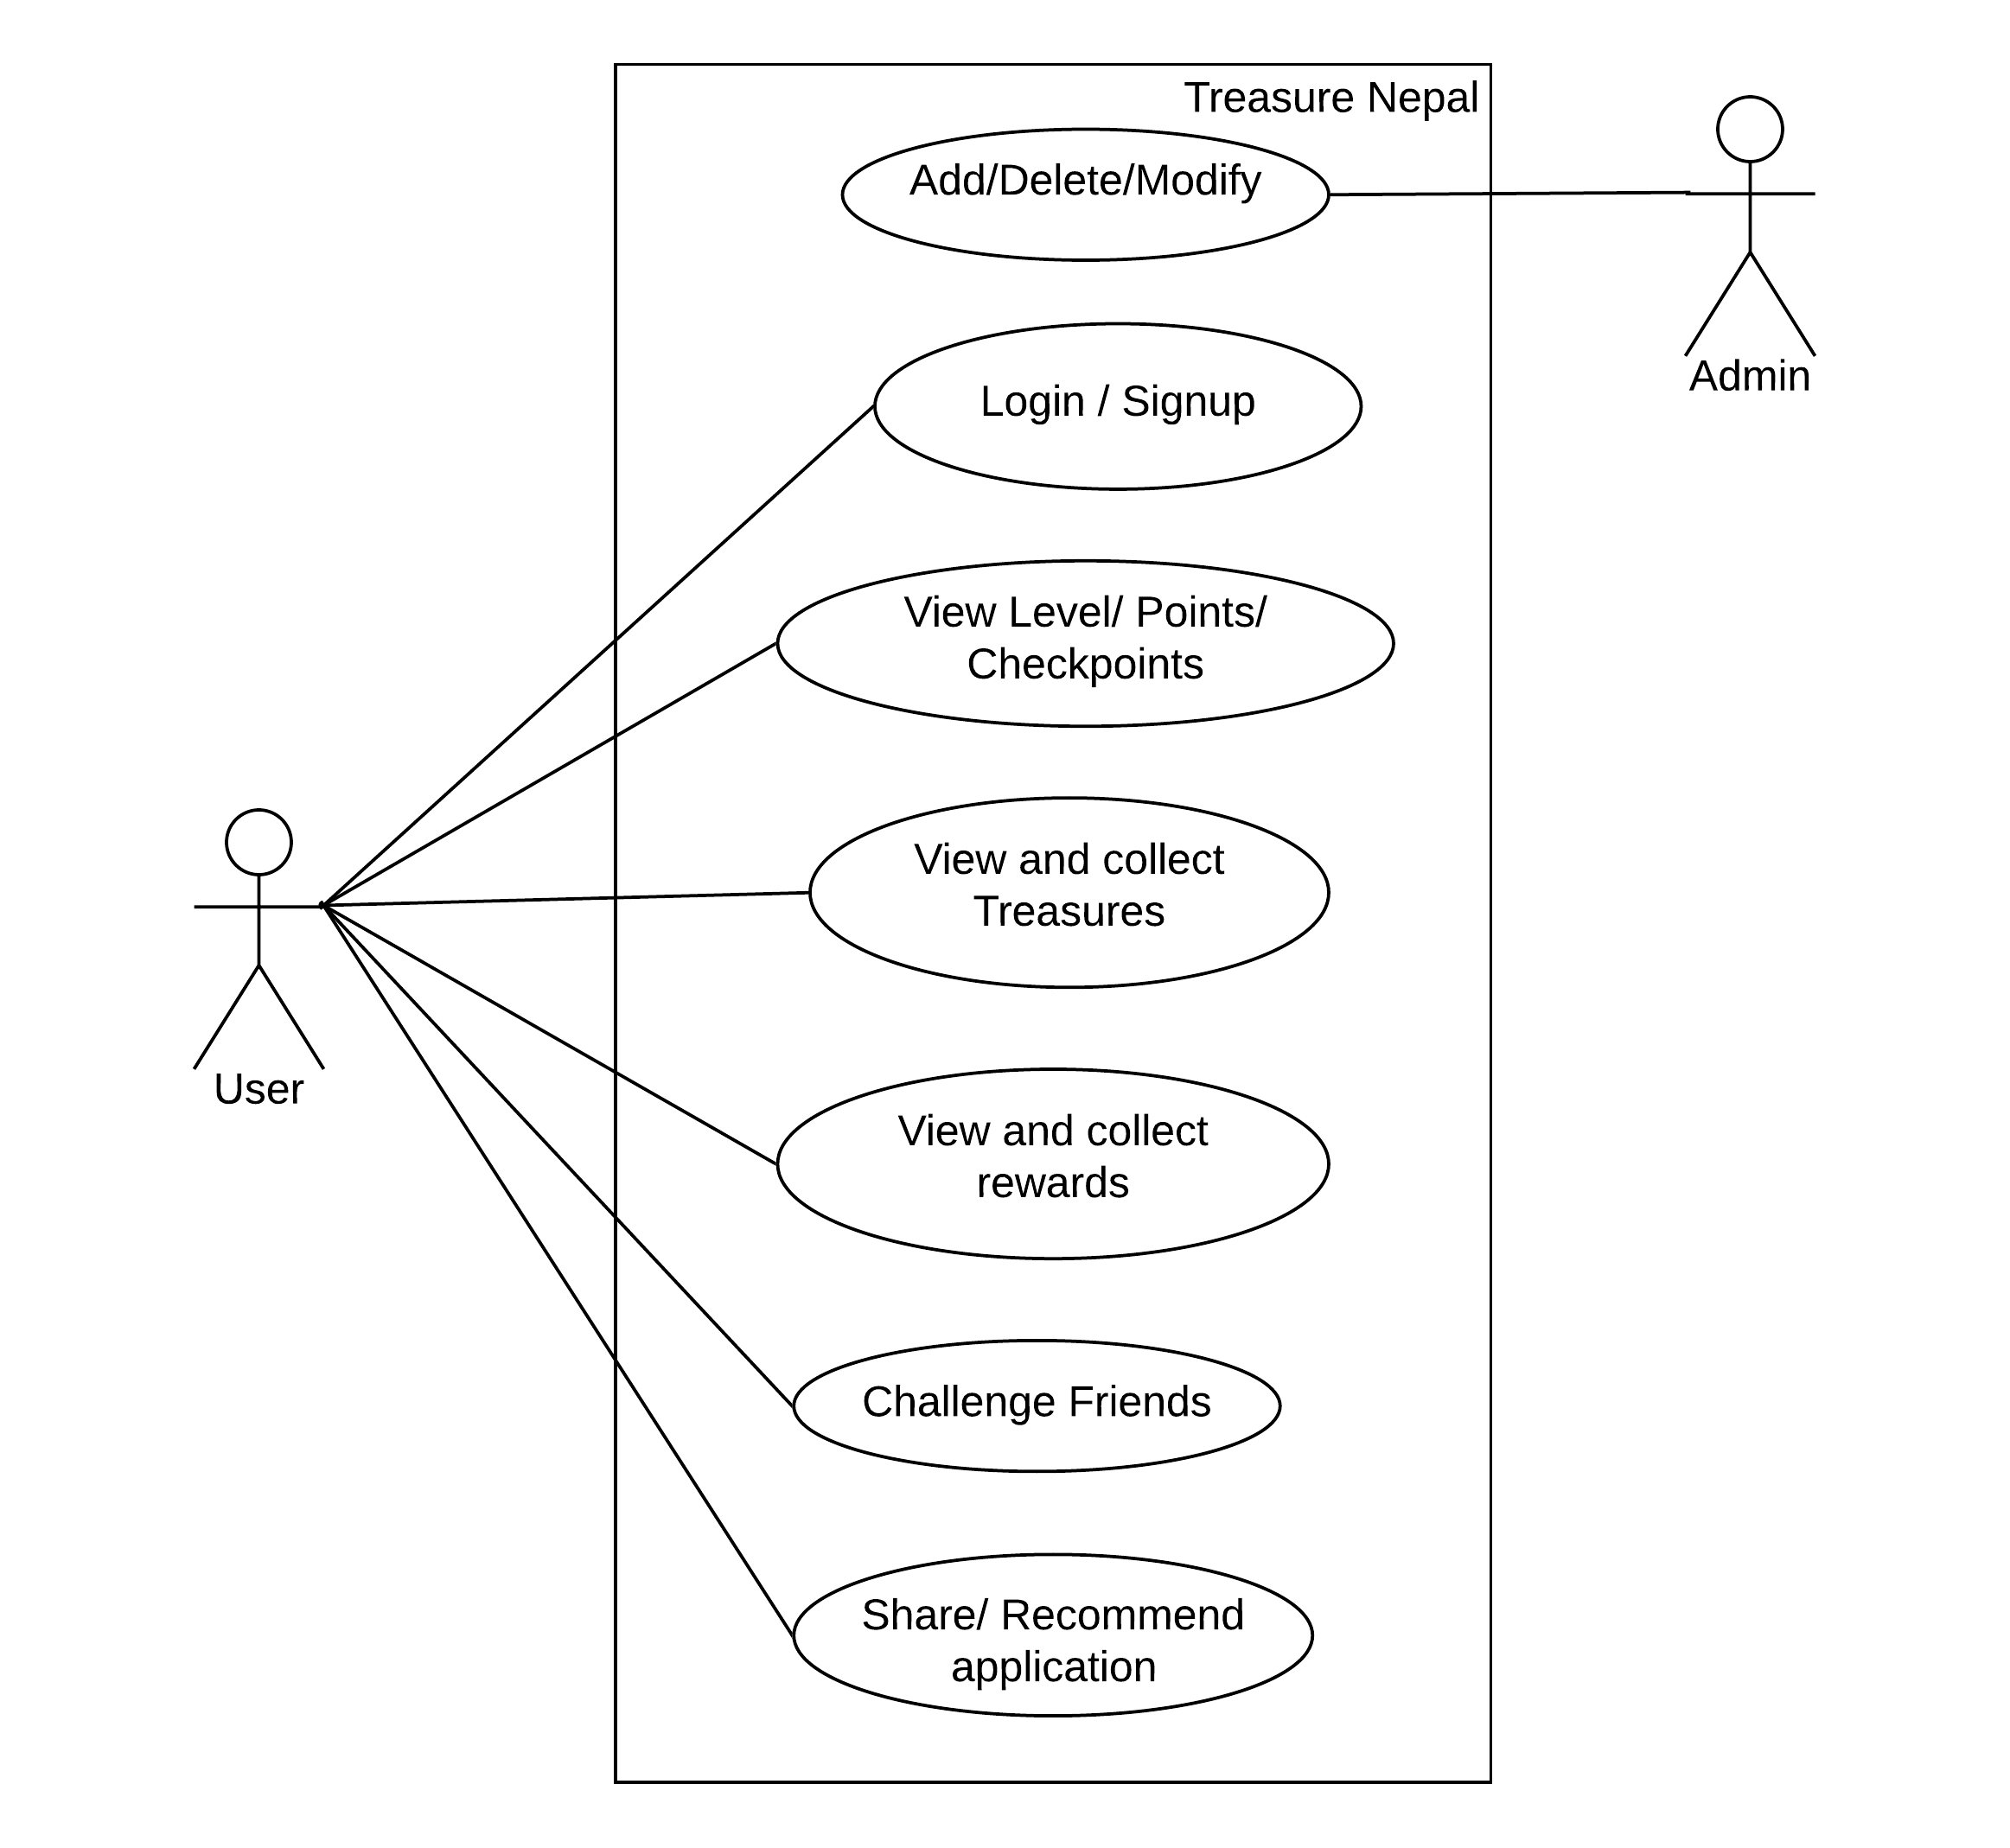
\includegraphics[width=\linewidth]{use-case-diagrams/all.png}
\centering
\caption{Use case diagram for overall application}
\label{fig:use-case-all}
\end{figure}

After a series of in depth analysis, we figured out that the two major parts in our application are the collection of treasures and rewards. Hence, we prepared the use case diagram for the scenario of treasure collection as shown in the Figure \ref{fig:use-case-treasure}. 


\begin{figure}[H]
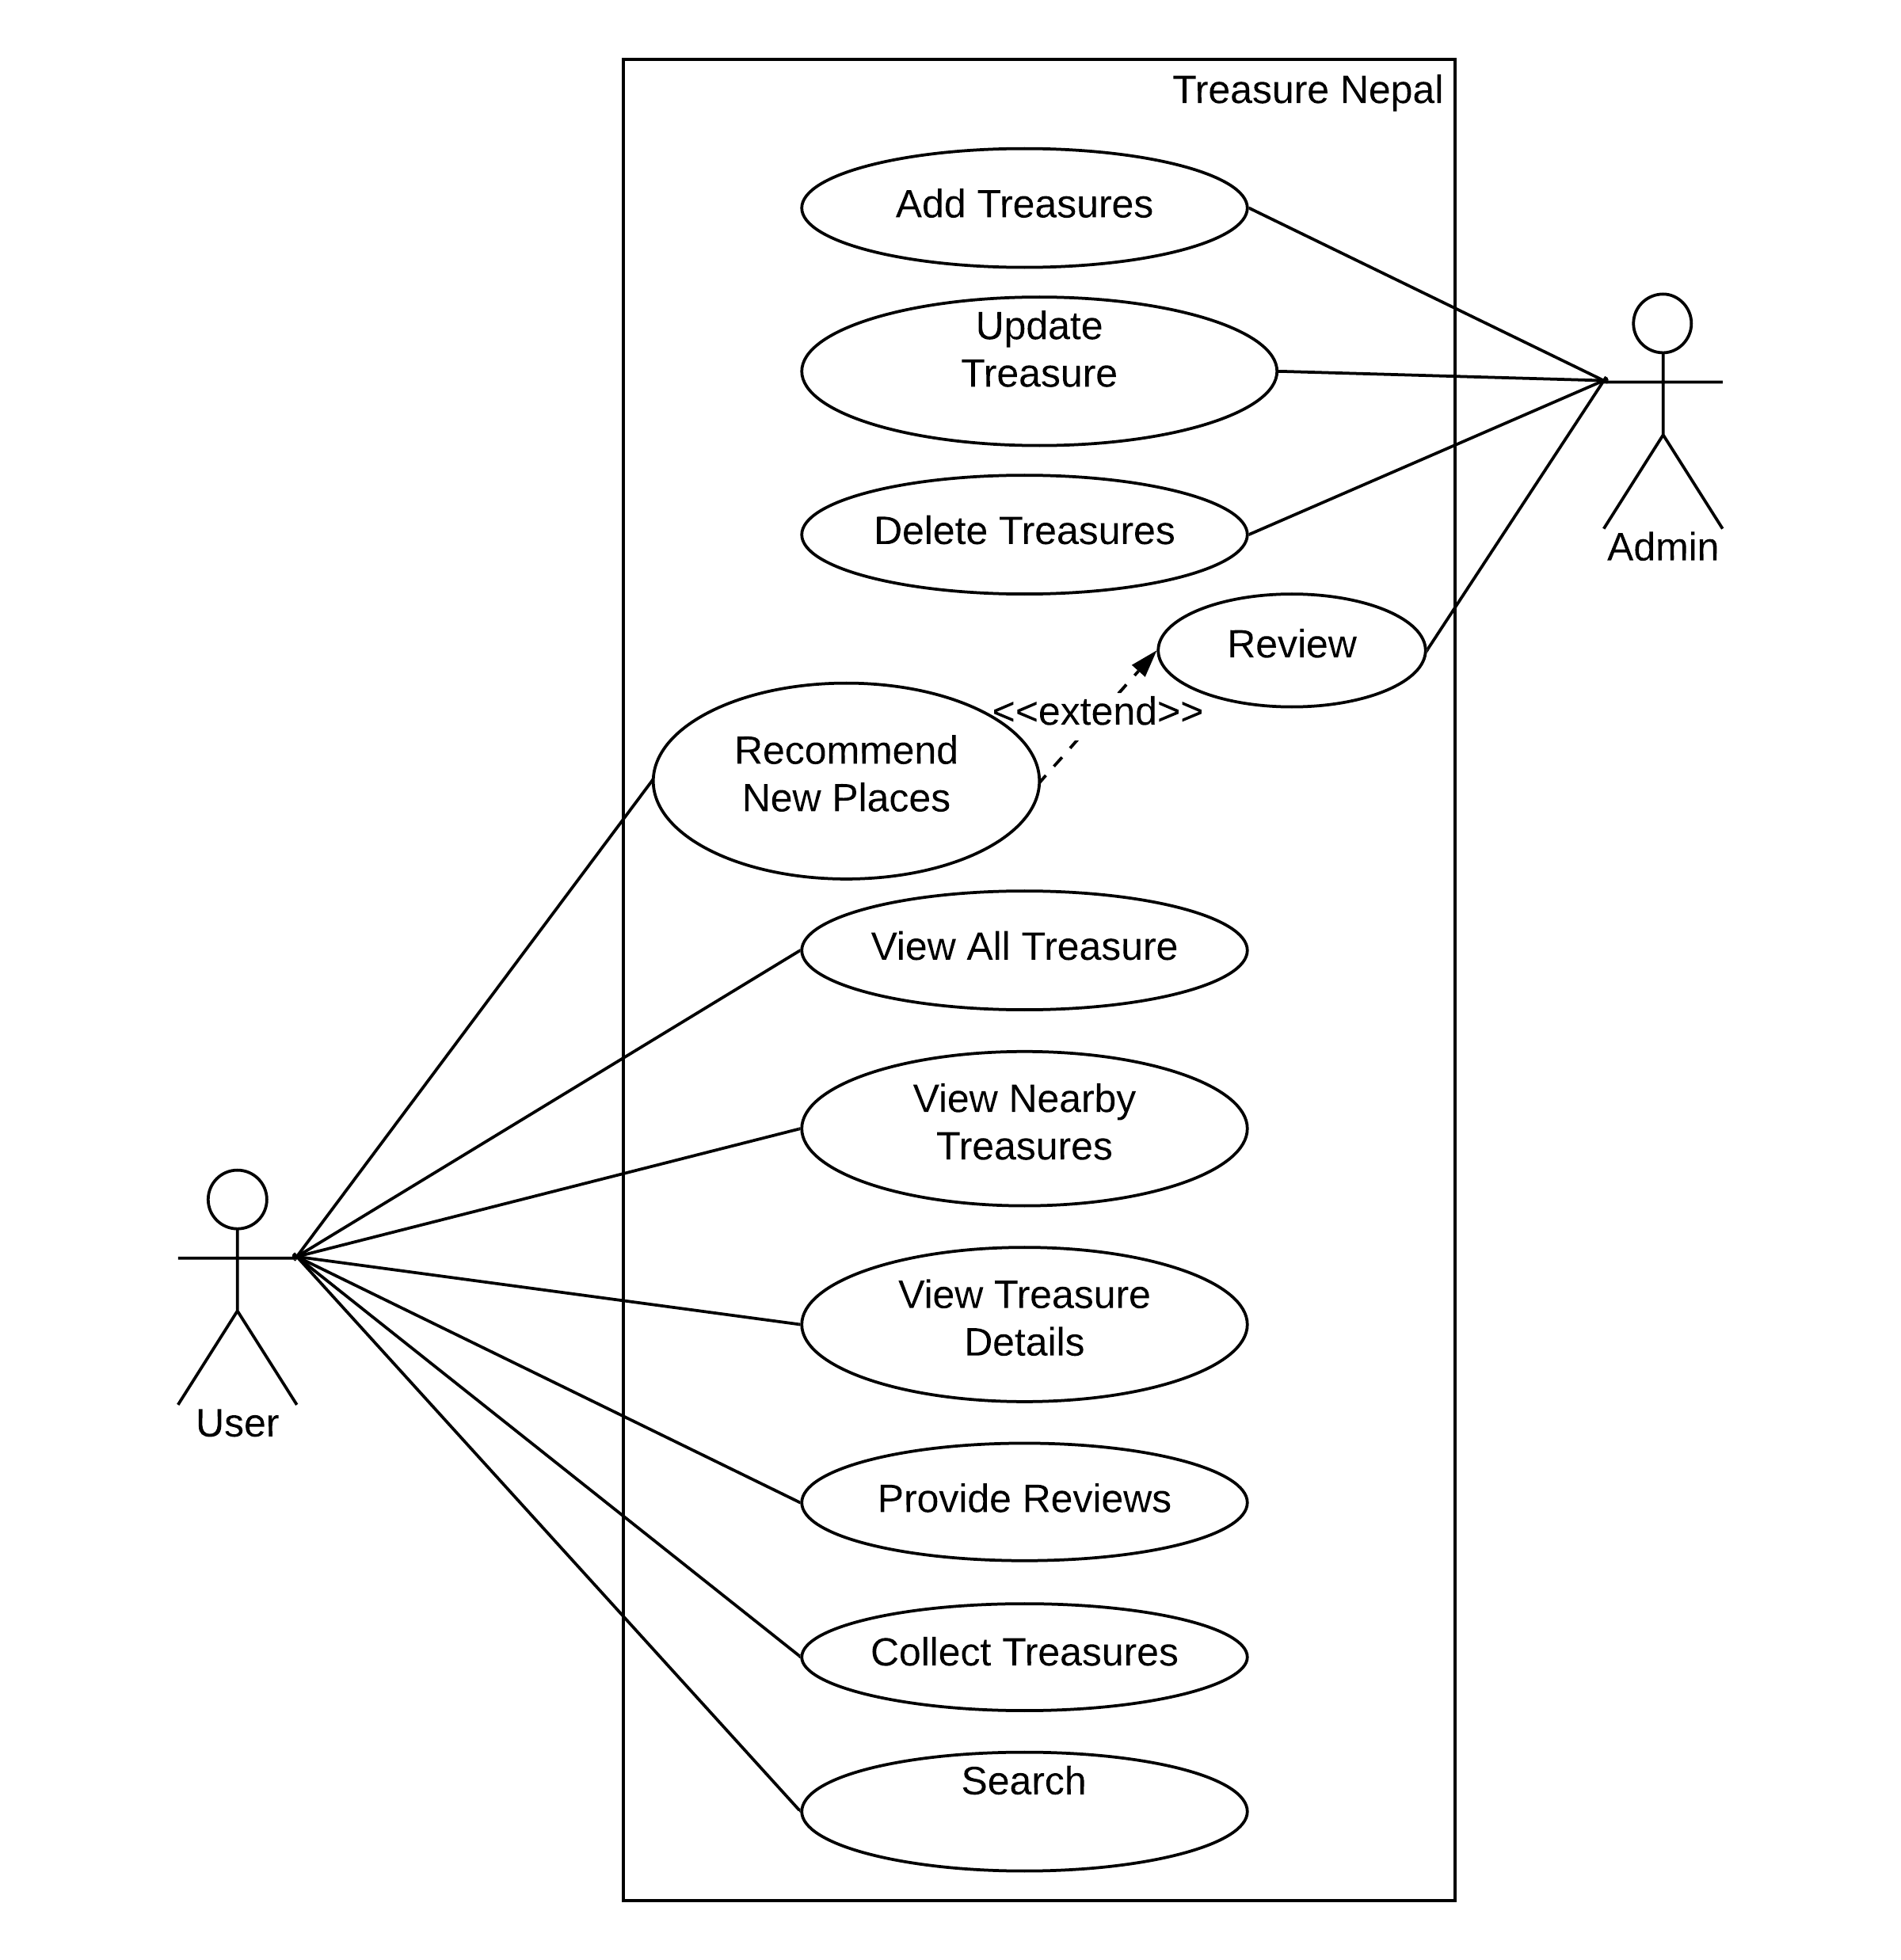
\includegraphics[width=\linewidth]{use-case-diagrams/treasure.png}
\centering
\caption{Use case diagram for treasure collection}
\label{fig:use-case-treasure}
\end{figure}

Next, we proceeded to draw use case digram for the scenario of reward collection as shown in Figure \ref{fig:use-case-reward}.

\begin{figure}[H]
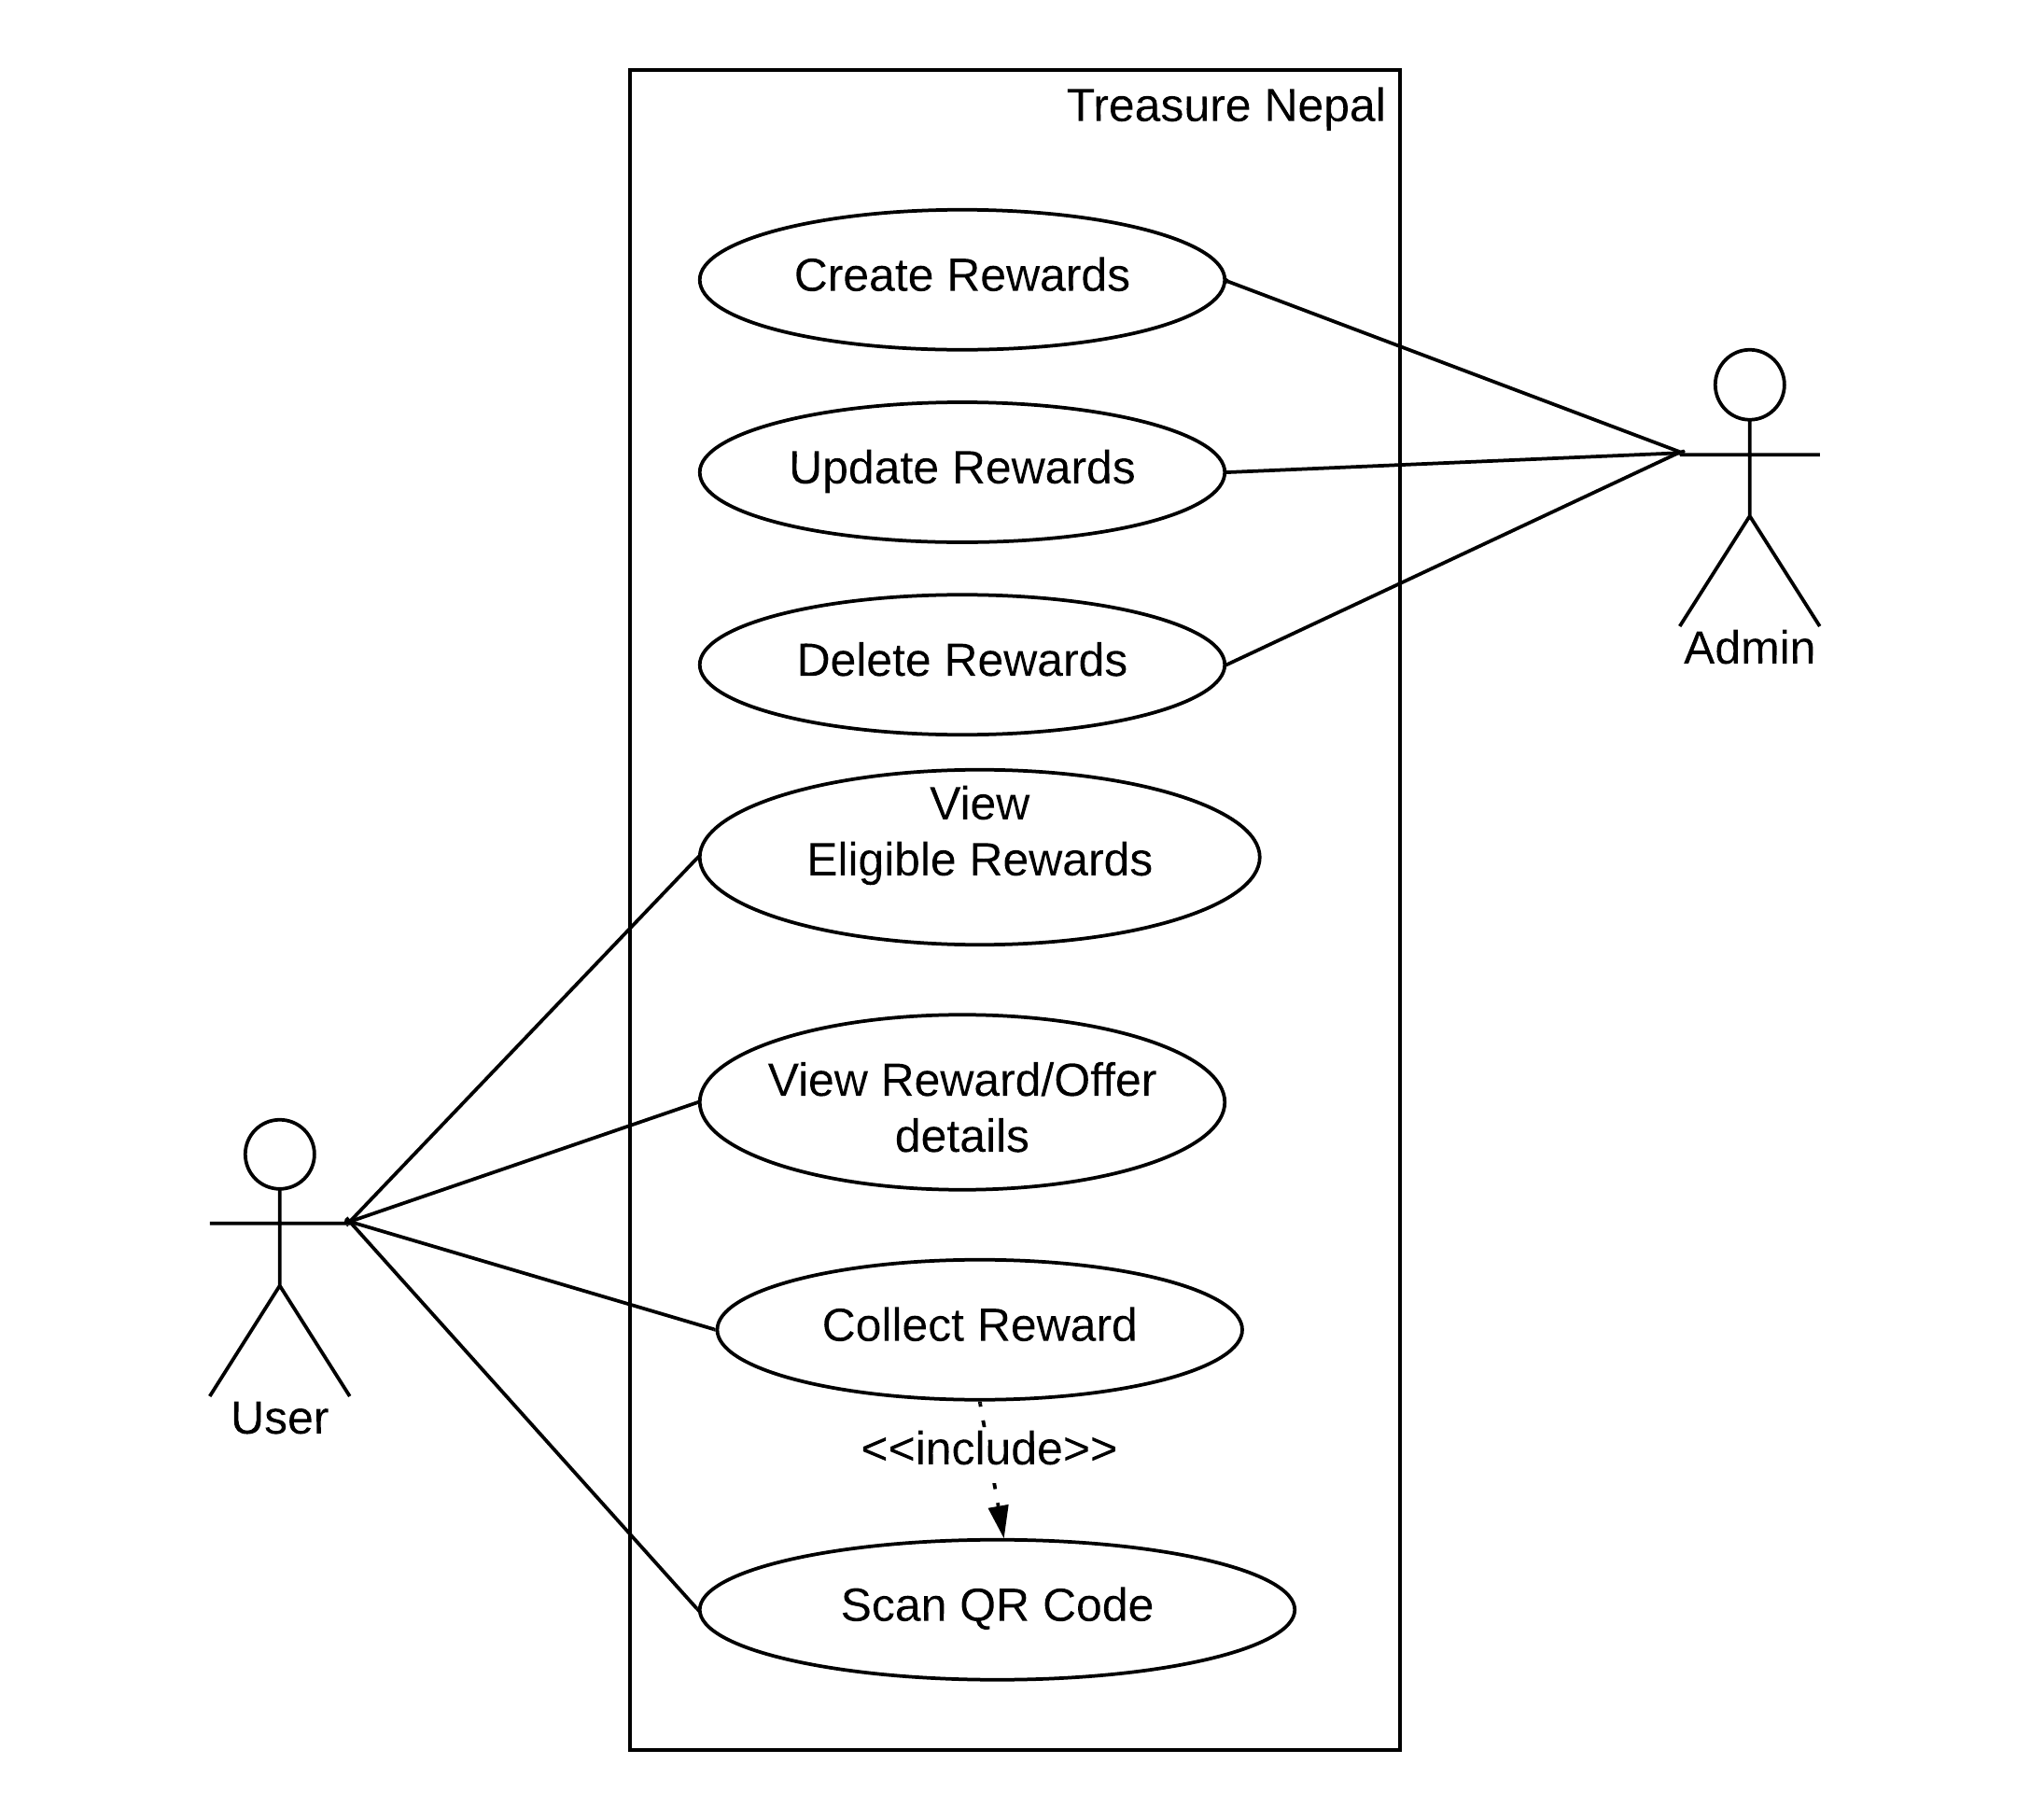
\includegraphics[width=\linewidth]{use-case-diagrams/reward.png}
\centering
\caption{Use case diagram for reward collection}
\label{fig:use-case-reward}
\end{figure}

%\subsection{Requirement Validation}

\subsubsection{Use Case Descriptions}
A use case description is the written description of how the users will interact with the system, what will the preconditions and postconditions be, what are the flow of actions needed to be performed along the main course of action, what are the alternative courses of flow of actions, and many more. It is generally prepared after the preparation of UML use case diagram. Each of the use case in the UML use case diagram needs a detailed description during this phase.

The tables that follow are the use case descriptions of various use cases shown earlier in subsection \ref{usecasediagrams} in diagrammatic form.

\begin{table}[H]
\begin{tabularx}{\linewidth}{|c|X|}
\hline
Name & Login                                                                                                                                                                                                                                                                               \\ \hline
ID                          & UC001                                                                                                                                                                                                                                                                                                       \\ \hline
Description                 & The user wants to login to the application using his/her account credentials                                                                                                                                                                                                                            \\ \hline
Actors                      & A: Application User (Tourist)                                                                                                                                                                                                                                                                                  \\ \hline
Frequency of Use            & High                                                                                                                                                                                                                                                                                                        \\ \hline
Trigger                     & User presses one of the Login buttons.                                                                                                                                                                                                                                                                      \\ \hline
Preconditions               & -                                                                                                                                                                                                                                                                                                           \\ \hline
Postconditions              & The user is successfully logged in to the application. \newline He/she is navigated to the Dashboard page.                                                                                                                                                         \\ \hline
Main Course                 & 1. User inputs his/her email and password in the login form.\newline 2. User presses the 'Login' button \newline 3. User is navigated to the Dashboard page                                                                                                            \\ \hline
Alternative Courses         & AC1: User presses 'Login via Google' button \newline AC2: User presses 'Login via Facebook' button                                                                                                                                                                   \\ \hline
Exceptions                  & EX1: Username/Password doesn't match\newline 1. User sees 'Invalid Credentials' message.\newline \newline EX2: Username/Password fields are blank \newline 1. User sees 'Fields cannot be blank' message\newline \newline EX3: The account doesn't exist. \newline 1. User sees 'Account doesn't exist' message\\ \hline
\end{tabularx}
\caption{Use Case: Login}
\label{uc-login}
\end{table}

\begin{table}[H]
\begin{tabularx}{\linewidth}{|c|X|}
\hline
Name                & Signup                                                                                                                                                                                                                      \\ \hline
ID                  & UC002                                                                                                                                                                                                                       \\ \hline
Description         & The user wants to register a new account in the application                                                                                                                                                                 \\ \hline
Actors              & A: Application User (Tourist)                                                                                                                                                                                                  \\ \hline
Frequency of Use    & Moderate                                                                                                                                                                                                                    \\ \hline
Trigger             & User presses one of the Register.                                                                                                                                                                                           \\ \hline
Preconditions       & -                                                                                                                                                                                                                           \\ \hline
Postconditions      & The user account is successfully created. \newline He/she is navigated to the Dashboard page.                                                                                                                                         \\ \hline
Main Course         & 1. User inputs his/her email, username and password in the register form. \newline 2. User taps the 'Register' button \newline 3. User completes the profile by providing name, address and nationality. \newline 4. User is navigated to Dashboard page. \\ \hline
Alternative Courses & AC1: User presses 'Login via Google' button \newline Same as AC1 of UC001 \newline \newline AC2: User presses 'Login via Facebook' button \newline Same as AC2 of UC002                                                                                            \\ \hline
Exceptions          & EX1: Email isn't valid \newline 1. User sees 'Invalid Email' message. \newline \newline EX2: Email or username is already used \newline 1. User sees 'Account already exists' message \newline \newline EX3: The input fields are blank. \newline 1. User sees 'Fields cannot be blank' message \\ \hline
\end{tabularx}
\caption{Use Case: Signup}
\label{uc-signup}
\end{table}

\begin{table}[H]
\begin{tabularx}{\linewidth}{|c|X|}
\hline
Name                & View Points and Position                                                                                                                                                                                                                      \\ \hline
ID                  & UC003                                                                                                                                                                                                                       \\ \hline
Description         & The user wants to view the points he has scored and his position in global leaderboard.                                                                                                                                                    \\ \hline
Actors              & A: Application User (Tourist)                                                                                                                                                                                                  \\ \hline
Frequency of Use    & High                                                                                                                                                                                                                    \\ \hline
Trigger             & User navigates to the Dashboard screen                                                                                                                                                                                           \\ \hline
Preconditions       & The user (A) is logged in with valid credentials                                                                                                                                                                                                                           \\ \hline
Postconditions      & The user views his/her points and position                                                                                                                                        \\ \hline
Main Course         & 1. User navigates to the Dashboard screen. \newline 2. User sees his/her points and position. \\ \hline
Alternative Courses & AC1: User refreshes the Dashboard screen \newline Same as main course                                                                                             \\ \hline
Exceptions          & EX1: Network error \newline User sees 'No internet connection' message, and cached points and position.  \\ \hline
\end{tabularx}
\caption{Use Case: View Points and Position}
\label{uc-view-points}
\end{table}

\begin{table}[H]
\begin{tabularx}{\linewidth}{|c|X|}
\hline
Name                & Share Application                                                                                                                                                                                                                      \\ \hline
ID                  & UC004                                                                                                                                                                                                                       \\ \hline
Description         & The user wants to share the application via email or other applications.                                                                                                                                                    \\ \hline
Actors              & A: Application User (Tourist)                                                                                                                                                                                                  \\ \hline
Frequency of Use    & Low                                                                                                                                                                                                                    \\ \hline
Trigger             & User taps 'Share' button                                                                                                                                                                                           \\ \hline
Preconditions       & -                                                                                                                                                                                                                           \\ \hline
Postconditions      & The user is prompted with a list of application to share with.                                                                                                                                        \\ \hline
\end{tabularx}
\caption{Use Case: Share Application}
\label{uc-view-points}
\end{table}

\begin{table}[H]
\begin{tabularx}{\linewidth}{|c|X|}
\hline
Name                & Add Treasures                                                                                                                                                                                                                      \\ \hline
ID                  & UC005                                                                                                                                                                                                                       \\ \hline
Description         & The actor wants to add a new treasure to database                                                                                                                                                    \\ \hline
Actors              & A: Database Administrator                                                                                                                                                                                                 \\ \hline
Frequency of Use    & High                                                                                                                                                                                                                    \\ \hline
Trigger             & User fills the form and presses 'Add' button in admin panel                                                                                                                                                                                           \\ \hline
Preconditions       & The administrator is authorized to make changes.                                                                                                                                                                                                                           \\ \hline
Postconditions      & A new treasure is added to the database                                                                                                                                        \\ \hline
Main Course         & 1. The admin goes to the admin panel. \newline 2. He/She fills up the form.  \newline 3. He/She clicks the 'Add Treasure' button \\ \hline
Alternative Courses & AC1: Admin cancels the addition of new treasure \newline Treasure is not added to database                                                                                             \\ \hline
Exceptions          & EX1: Duplicate Entry \newline Admin is prompted with 'Duplicate Entry' message \\ \hline
\end{tabularx}
\caption{Use Case: Add Treasure}
\label{uc-add-treasure}
\end{table}


\begin{table}[H]
\begin{tabularx}{\linewidth}{|c|X|}
\hline
Name                & Update Treasure                                                                                                                                                                                                                      \\ \hline
ID                  & UC006                                                                                                                                                                                                                       \\ \hline
Description         & The actor wants to update information of existing treasure                                                                                                                                                    \\ \hline
Actors              & A: Database Administrator                                                                                                                                                                                                 \\ \hline
Frequency of Use    & Moderate                                                                                                                                                                                                                    \\ \hline
Trigger             & Admin clicks 'edit' icon to edit a treasure                                                                                                                                                                                           \\ \hline
Preconditions       & The administrator is authorized to make changes.                                                                                                                                                                                     \\ \hline
Postconditions      & A treasure is updated in the database with new information                                                                                                                                       \\ \hline
Main Course         & 1. The admin goes to the admin panel. \newline 2. He/She views the treasure to update.  \newline 3. He/She clicks the 'Edit Button' button \newline 4. He/She fills the edit form \newline 5. He/She submits by clicking 'Update' button. \\ \hline
Alternative Courses & AC1: Admin cancels the modification of treasure \newline Treasure is not modified in the database                                                                                             \\ \hline
Exceptions          & EX1: Duplicate Entry \newline Admin is prompted with 'Duplicate Entry' message \\ \hline
\end{tabularx}
\caption{Use Case: Update Treasure}
\label{uc-update-treasure}
\end{table}

\begin{table}[H]
\begin{tabularx}{\linewidth}{|c|X|}
\hline
Name                & Delete Treasure                                                                                                                                                                                                                      \\ \hline
ID                  & UC007                                                                                                                                                                                                                       \\ \hline
Description         & The actor wants to delete an existing treasure                                                                                                                                                    \\ \hline
Actors              & A: Database Administrator                                                                                                                                                                                                 \\ \hline
Frequency of Use    & Low                                                                                                                                                                                                                    \\ \hline
Trigger             & Admin clicks 'delete' icon to delete a treasure                                                                                                                                                                                           \\ \hline
Preconditions       & The administrator is authorized to make changes.                                                                                                                                                                                     \\ \hline
Postconditions      & The treasure is deleted from the database                                                                                                                                        \\ \hline
Main Course         & 1. The admin goes to the admin panel. \newline 2. He/She views the treasure to delete.  \newline 3. He/She clicks the 'Delete' button \newline 4. He/She will click 'Yes' to the confirmation prompt  \\ \hline
Alternative Courses & AC1: Admin presses 'No' during the confirmation \newline Treasure is not deleted from the database                                                                                             \\ \hline
Exceptions          & EX1: Duplicate Entry \newline Admin is prompted with 'Duplicate Entry' message \\ \hline
\end{tabularx}
\caption{Use Case: Delete Treasure}
\label{uc-delete-treasure}
\end{table}

\begin{table}[H]
\begin{tabularx}{\linewidth}{|c|X|}
\hline
Name                & View Treasures                                                                                                                                                                                                                      \\ \hline
ID                  & UC008                                                                                                                                                                                                                       \\ \hline
Description         & The actor wants to view available treasures in a map                                                                                                                                                   \\ \hline
Actors              & A: Application user (Tourist)                                                                                                                                                                                                 \\ \hline
Frequency of Use    & High                                                                                                                                                                                                                    \\ \hline
Trigger             & User navigates to 'Treasure' screen                                                                                                                                                                                           \\ \hline
Preconditions       & The user is logged in                                                                                                                                                                                                                          \\ \hline
Postconditions      & The user sees several treasure pins in the interactive map in the user's current location                                                                                                                                      \\ \hline
Main Course         & 1. The user navigates to 'Treasure' screen. \newline 2. He/She gives permission for location access. \\ \hline
Alternative Courses & AC1: The user denies the location access \newline The map is centered on the default location but the treasures are still visible                                                                                            \\ \hline
\end{tabularx}
\caption{Use Case: View Treasures}
\label{uc-view-treasures}
\end{table}


\begin{table}[H]
\begin{tabularx}{\linewidth}{|c|X|}
\hline
Name                & View Treasure Details                                                                                                                                                                                                                     \\ \hline
ID                  & UC009                                                                                                                                                                                                                       \\ \hline
Description         & The actor wants to view the detailed information about a treasure                                                                                                                                                   \\ \hline
Actors              & A: Application user (Tourist)                                                                                                                                                                                                 \\ \hline
Frequency of Use    & High                                                                                                                                                                                                                    \\ \hline
Trigger             & User presses 'View details' button on the card displaying the treasure.                                                                                                                                                                                           \\ \hline
Preconditions       & The user is logged in                                                                                                                                                                                                                          \\ \hline
Postconditions      & The user sees location, points, distance to, images and other treasure details                                                                                                                                      \\ \hline
Main Course         & 1. The user navigates to 'Treasure' screen. \newline 2. He/She gives permission for location access. \newline 3. He/She sees a number of treasures on location map. \newline 4. He/She taps on a pin in the map. \newline 5. The card showing the brief info about the treasure pops up. \newline 6. The user taps 'View Details' button.\\ \hline
Alternative Courses & AC1: The user denies the location access \newline Similar to AC1 of UC008                                                                                            \\ \hline
\end{tabularx}
\caption{Use Case: View Treasure Details}
\label{uc-view-treasure-details}
\end{table}

\begin{table}[H]
\begin{tabularx}{\linewidth}{|c|X|}
\hline
Name                & Scan QR Code                                                                                                                                                                                                                     \\ \hline
ID                  & UC010                                                                                                                                                                                                                       \\ \hline
Description         & The actor scans the QR code corresponding to a treasure or a reward.                                                                                                                                                   \\ \hline
Actors              & A: Application user (Tourist)                                                                                                                                                                                                 \\ \hline
Frequency of Use    & High                                                                                                                                                                                                                    \\ \hline
Trigger             & User navigates to the Scan screen.                                                                                                                                                                                           \\ \hline
Preconditions       & 1. The user is logged in  \newline 2. The current location of the user is accessible                                                                                                                                                                                                \\ \hline
Postconditions      & UC011 is triggered if the QR corresponds to a treasure. \newline UC020 is called if QR corresponds to a reward.                                                                                                                                      \\ \hline
Main Course         & 1. The user navigates to 'Scan' screen. \newline 2. He/She gives permission for camera access. \newline 3. He/She scans the QR code. \\ \hline
Alternative Courses & AC1: The user denies the camera access \newline User sees 'Camera access denied' screen.                                                                                            \\ \hline
\end{tabularx}
\caption{Use Case: View Treasure Details}
\label{uc-view-treasure-details}
\end{table}

\begin{table}[H]
\begin{tabularx}{\linewidth}{|c|X|}
\hline
Name                & Collect Treasure                                                                                                                                                                                                                     \\ \hline
ID                  & UC011                                                                                                                                                                                                                       \\ \hline
Description         & The actor collects a treasure to his/her account                                                                                                                                                   \\ \hline
Actors              & A: Application user (Tourist)                                                                                                                                                                                                 \\ \hline
Frequency of Use    & High                                                                                                                                                                                                                    \\ \hline
Trigger             & UC010 (The QR code corresponds to a Treasure)                                                                                                                                                                                           \\ \hline
Preconditions       & 1. UC010  \newline 2. The user's location is within the permitted distance from the location of treasure                                                                                                                                                                                                                        \\ \hline
Postconditions      & The user sees that the treasure is collected and the point increases.                                                                                                                                       \\ \hline
Main Course         & 1. The user scans the QR code. \newline 2. He/She views the 'Validating, please wait' message. \newline 3. He/She sees that the treasure is successfully collected. \newline 4. He/She is navigated to the Dashboard. \newline UC003 is triggered. \\ \hline
Alternative Courses & AC1: QR code is invalid \newline User will continue to see the Scan screen, nothing happens. \newline                                                                                           \\ \hline
\end{tabularx}
\caption{Use Case: Collect Treasure}
\label{uc-collect-treasure}
\end{table}

\begin{table}[H]
\begin{tabularx}{\linewidth}{|c|X|}
\hline
Name                & Search Treasure                                                                                                                                                                                                                     \\ \hline
ID                  & UC012                                                                                                                                                                                                                       \\ \hline
Description         & The actor wans to search a treasure by a search query                                                                                                                                                   \\ \hline
Actors              & A: Application user (Tourist)                                                                                                                                                                                                 \\ \hline
Frequency of Use    & High                                                                                                                                                                                                                    \\ \hline
Trigger             & The user types something in the search bar and presses search icon                                                                                                                                                                                           \\ \hline
Preconditions       & 1. The user is logged in                                                                                                                                                                                                                         \\ \hline
Postconditions      & The user sees the treasures that match his/her search query                                                                                                                                      \\ \hline
Main Course         & 1. The user types in a search query. \newline 2. He/She taps the search icon. \newline 3. He/She sees that the treasures that match the query. \\ \hline
\end{tabularx}
\caption{Use Case: Search Treasure}
\label{uc-search-treasure}
\end{table}


\begin{table}[H]
\begin{tabularx}{\linewidth}{|c|X|}
\hline
Name                & Add Reward                                                                                                                                                                                                                      \\ \hline
ID                  & UC013                                                                                                                                                                                                                       \\ \hline
Description         & The actor wants to add a new reward to database                                                                                                                                                    \\ \hline
Actors              & A: Database Administrator                                                                                                                                                                                                 \\ \hline
Frequency of Use    & High                                                                                                                                                                                                                    \\ \hline
Trigger             & User fills the form and presses 'Add' button in admin panel                                                                                                                                                                                           \\ \hline
Preconditions       & The administrator is authorized to make changes.                                                                                                                                                                                                                           \\ \hline
Postconditions      & A new reward is added to the database                                                                                                                                        \\ \hline
Main Course         & 1. The admin goes to the admin panel. \newline 2. He/She fills up the form.  \newline 3. He/She clicks the 'Add Reward' button \\ \hline
Alternative Courses & AC1: Admin cancels the addition of new reward \newline Reward is not added to database                                                                                             \\ \hline
Exceptions          & EX1: Duplicate Entry \newline Admin is prompted with 'Duplicate Entry' message \\ \hline
\end{tabularx}
\caption{Use Case: Add Reward}
\label{uc-add-reward}
\end{table}


\begin{table}[H]
\begin{tabularx}{\linewidth}{|c|X|}
\hline
Name                & Update Reward                                                                                                                                                                                                                      \\ \hline
ID                  & UC014                                                                                                                                                                                                                       \\ \hline
Description         & The actor wants to update information of existing reward                                                                                                                                                    \\ \hline
Actors              & A: Database Administrator                                                                                                                                                                                                 \\ \hline
Frequency of Use    & Moderate                                                                                                                                                                                                                    \\ \hline
Trigger             & Admin clicks 'edit' icon to edit a reward                                                                                                                                                                                           \\ \hline
Preconditions       & The administrator is authorized to make changes.                                                                                                                                                                                     \\ \hline
Postconditions      & The reward is updated in the database with new information                                                                                                                                       \\ \hline
Main Course         & 1. The admin goes to the admin panel. \newline 2. He/She views the reward to update.  \newline 3. He/She clicks the 'Edit Button' button \newline 4. He/She fills the edit form \newline 5. He/She submits by clicking 'Update Reward' button. \\ \hline
Alternative Courses & AC1: Admin cancels the modification of reward \newline Reward is not modified in the database                                                                                             \\ \hline
Exceptions          & EX1: Duplicate Entry \newline Admin is prompted with 'Duplicate Entry' message \\ \hline
\end{tabularx}
\caption{Use Case: Update Reward}
\label{uc-update-reward}
\end{table}

\begin{table}[H]
\begin{tabularx}{\linewidth}{|c|X|}
\hline
Name                & Delete Reward                                                                                                                                                                                                                      \\ \hline
ID                  & UC015                                                                                                                                                                                                                       \\ \hline
Description         & The actor wants to delete an existing reward                                                                                                                                                    \\ \hline
Actors              & A: Database Administrator                                                                                                                                                                                                 \\ \hline
Frequency of Use    & Low                                                                                                                                                                                                                    \\ \hline
Trigger             & Admin clicks 'delete' icon to delete a reward                                                                                                                                                                                           \\ \hline
Preconditions       & The administrator is authorized to make changes.                                                                                                                                                                                     \\ \hline
Postconditions      & The reward is deleted from the database                                                                                                                                        \\ \hline
Main Course         & 1. The admin goes to the admin panel. \newline 2. He/She views the reward to delete.  \newline 3. He/She clicks the 'Delete' button \newline 4. He/She will click 'Yes' to the confirmation prompt  \\ \hline
Alternative Courses & AC1: Admin presses 'No' during the confirmation \newline Reward is not deleted from the database                                                                                             \\ \hline
Exceptions          & EX1: Duplicate Entry \newline Admin is prompted with 'Duplicate Entry' message \\ \hline
\end{tabularx}
\caption{Use Case: Delete Reward}
\label{uc-delete-reward}
\end{table}

\begin{table}[H]
\begin{tabularx}{\linewidth}{|c|X|}
\hline
Name                & View Eligible Rewards                                                                                                                                                                                                                      \\ \hline
ID                  & UC016                                                                                                                                                                                                                       \\ \hline
Description         & The actor wants to view the list rewards he/she has earned                                                                                                                                                 \\ \hline
Actors              & A: Application user (Tourist)                                                                                                                                                                                                 \\ \hline
Frequency of Use    & High                                                                                                                                                                                                                    \\ \hline
Trigger             & User navigates to 'Rewards' screen                                                                                                                                                                                           \\ \hline
Preconditions       & The user is logged in                                                                                                                                                                                                                          \\ \hline
Postconditions      & The user sees a list of the rewards that are available to him/her                                                                                                                                      \\ \hline
Alternative Courses & AC1: There are no rewards that the user has collected \newline The user sees 'You have no rewards' message                                                                                           \\ \hline
\end{tabularx}
\caption{Use Case: View Eligible Rewards}
\label{uc-view-rewards}
\end{table}


\begin{table}[H]
\begin{tabularx}{\linewidth}{|c|X|}
\hline
Name                & View Reward Details                                                                                                                                                                                                                     \\ \hline
ID                  & UC017                                                                                                                                                                                                                       \\ \hline
Description         & The actor wants to view the detailed information about a reward                                                                                                                                                   \\ \hline
Actors              & A: Application user (Tourist)                                                                                                                                                                                                 \\ \hline
Frequency of Use    & High                                                                                                                                                                                                                    \\ \hline
Trigger             & User presses the card displaying the reward.                                                                                                                                                                                           \\ \hline
Preconditions       & The user is logged in                                                                                                                                                                                                                          \\ \hline
Postconditions      & The user sees location, offers, distance to, images and other reward details                                                                                                                                      \\ \hline
\end{tabularx}
\caption{Use Case: View Reward Details}
\label{uc-view-reward-details}
\end{table}


\begin{table}[H]
\begin{tabularx}{\linewidth}{|c|X|}
\hline
Name                & Collect Reward                                                                                                                                                                                                                     \\ \hline
ID                  & UC018                                                                                                                                                                                                                       \\ \hline
Description         & The actor redeems the reward offered to him/her                                                                                                                                                  \\ \hline
Actors              & A: Application user (Tourist)                                                                                                                                                                                                 \\ \hline
Frequency of Use    & High                                                                                                                                                                                                                    \\ \hline
Trigger             & UC010 (The QR code corresponds to a Reward)                                                                                                                                                                                           \\ \hline
Preconditions       & 1. UC010                                                                                                                                                                                                                        \\ \hline
Postconditions      & The user gets the voucher code by which he/she can get the promised offer.                                                                                                                                       \\ \hline
Alternative Courses & AC1: QR code is invalid \newline User will continue to see the Scan screen, nothing happens. \newline                                                                                           \\ \hline
\end{tabularx}
\caption{Use Case: Collect Reward}
\label{uc-collect-reward}
\end{table}

\begin{table}[H]
\begin{tabularx}{\linewidth}{|c|X|}
\hline
Name                & Search Rewards                                                                                                                                                                                                                     \\ \hline
ID                  & UC019                                                                                                                                                                                                                       \\ \hline
Description         & The actor wans to search a reward by a search query                                                                                                                                                   \\ \hline
Actors              & A: Application user (Tourist)                                                                                                                                                                                                 \\ \hline
Frequency of Use    & High                                                                                                                                                                                                                    \\ \hline
Trigger             & The user types something in the search bar and presses search icon                                                                                                                                                                                           \\ \hline
Preconditions       & 1. The user is logged in                                                                                                                                                                                                                         \\ \hline
Postconditions      & The user sees the rewards he/she is eligible to, and that match his/her search query                                                                                                                                      \\ \hline
Main Course         & 1. The user types in a search query. \newline 2. He/She taps the search icon. \newline 3. He/She sees that the rewards that match the query. \\ \hline
\end{tabularx}
\caption{Use Case: Search Rewards}
\label{uc-search-rewards}
\end{table}













\pagebreak
\section{Design}
The design phase in software development life cycle follows after the Software Requirements Specification (SRS) documentation is ready. In this phase, the SRS document is used as an input and a detailed software architecture that will implement the requirements in SRS document is designed. Moreover, the design of the classes, interfaces, databases, etc. are also performed in this phase. The subsections that follow describe the various process followed during the design phase of our project.

\subsection{Architectural Design}
The application has been built upon the client-server web architecture, as illustrated in Figure \ref{fig:arch}.

\begin{figure}[H]
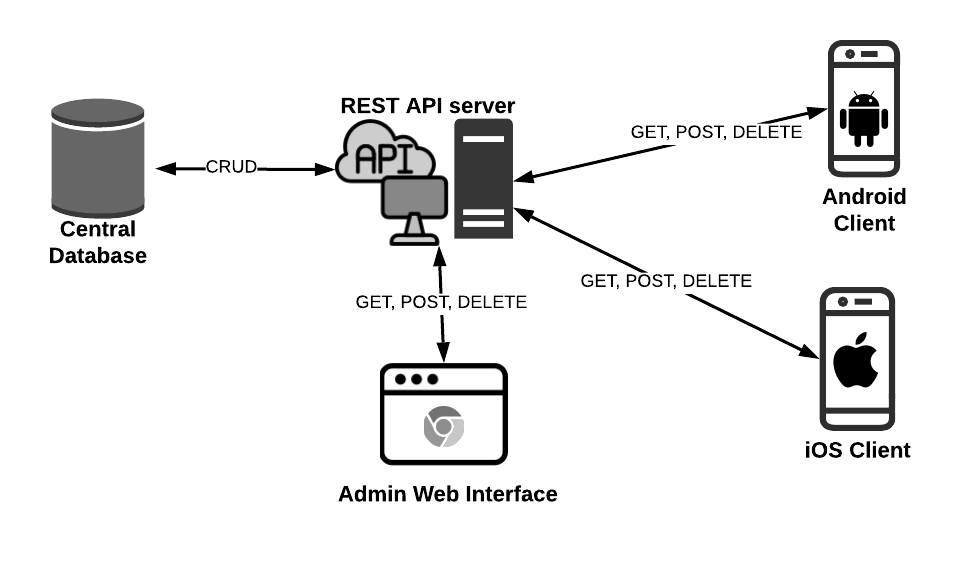
\includegraphics[width=\linewidth]{architecture}
\centering
\caption{Technical architecture of the application}
\label{fig:arch}
\end{figure}

\subsubsection{API server}
At the heart of the architecture lies the RESTful API server which communicates directly with the central database where all the data is stored. The mobile applications do not access the database directly, but via the API service. The clients send HTTP requests like GET, POST, PUT, PATCH and DELETE, while the API server processes those requests and return the data in JSON format.

\subsubsection{Database Tier}
The central database holds all the data related to our project. The Create, Read, Update and Delete (CRUD) operations on the database are performed through the RESTful API service. Hence, the database logic is implemented in this tier. Also, the relationship between various relations are implemented by use of foreign keys in the database. The database system used in this tier was Relational Database Management System (RDBMS), and the language used was Structured Query Language(SQL).

\subsubsection{Android/iOS Applications}
The users who have a mobile phone or tablet running Android or iOS will install the android application developed as part of our project in order to use the services provided by the API server. The client sends HTTP requests over the internet to access various endpoints in the API server and then display the results obtained in a way that is intuitive to the user. Hence, all the presentation logic are implemented in this tier.

\subsubsection{Admin Interface}
This module is the interface through which the treasures and rewards are added, updated and deleted. This module is only used by the administrators or data entry clerks in order to add new data or update the existing ones. In the present scope, we have used Django's in-built admin interface for all the data entry purposes.

\subsection{Database Design}
Database design is the process of designing the schema and architecture of the database to be used in the software project. It generally follows after a foundation of technical architecture is laid out with the help of the SRS document.

Figure \ref{fig:db-schema} illustrates the database schema used for the application. 

\begin{figure}[H]
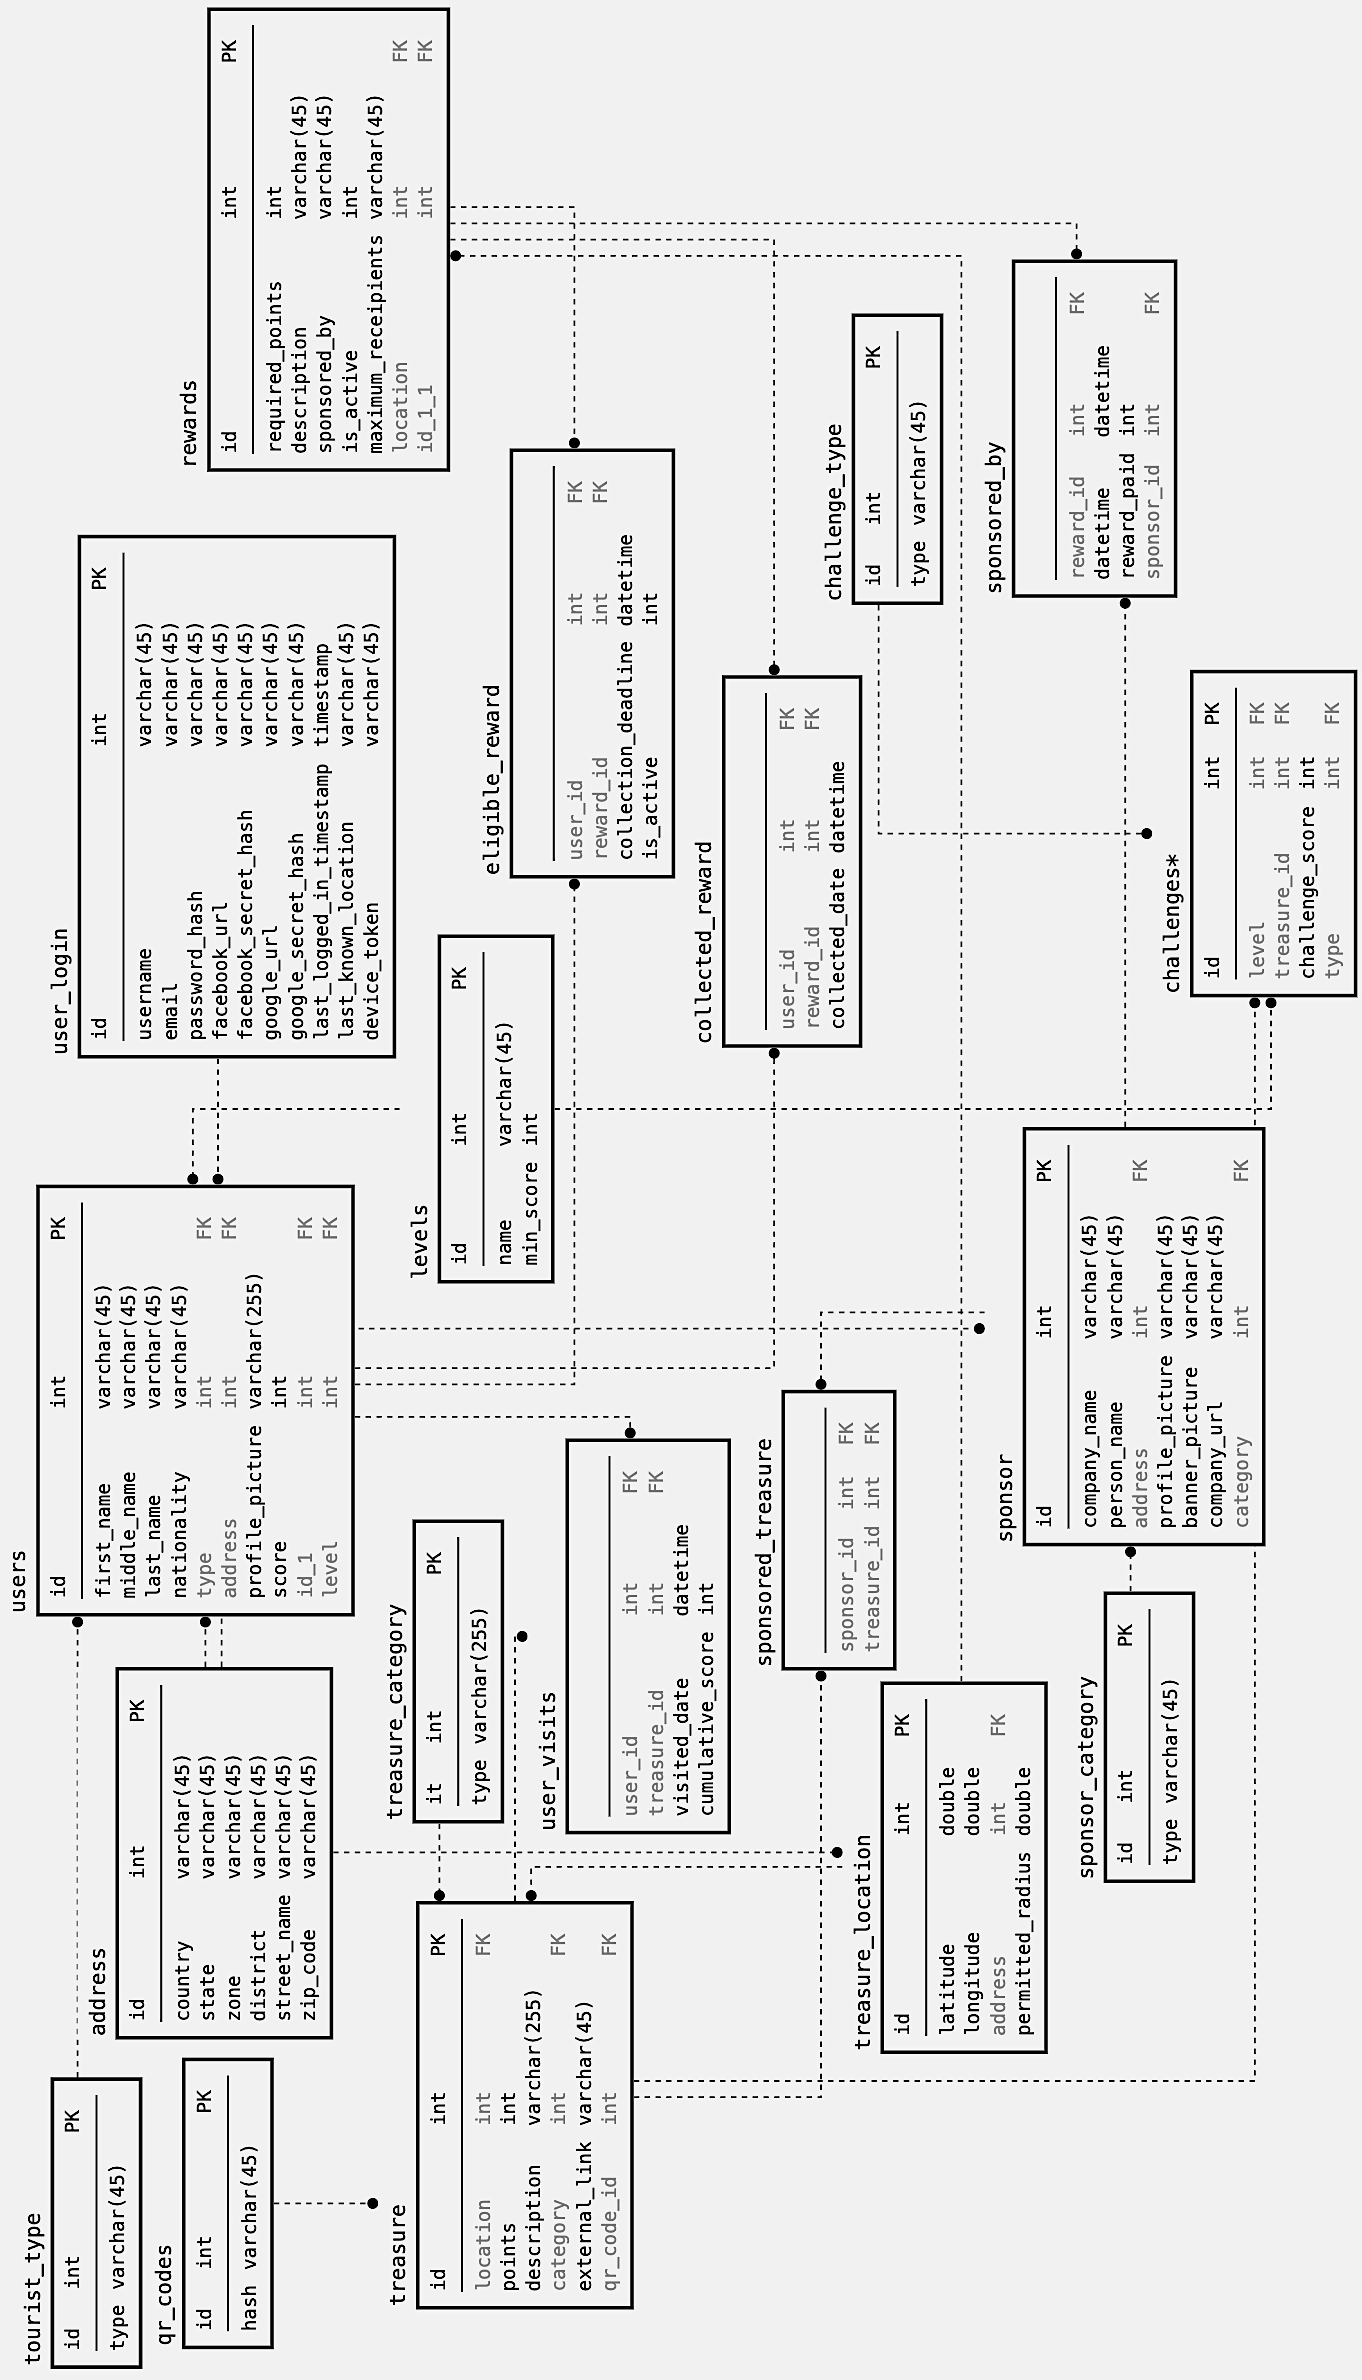
\includegraphics[height=0.8\paperheight, keepaspectratio]{db/schema.png}
\centering
\caption{Schema used in backend database}
\label{fig:db-schema}
\end{figure}

\subsection{System Design}
After the design of the database, we divided the overall project into different modules. The next task performed was to design how these different modules would be implemented in our project, what will be the flow of control and data, and so on. For designing a system, we made use of various tools such as UML System Sequence Diagrams (SSD).

\subsubsection{UML Sequence Diagrams}
Sequence diagrams are a category of UML diagrams that show the interaction between objects or modules of a software in time sequence. The interactions occur in a series of method calls (also called as messages) and responses. Diagrammatically, the messages are represented by a solid line while the responses are represented by a dashed line. The figures that follow show how the interaction between different object happen during different usage scenarios.

\begin{figure}[H]
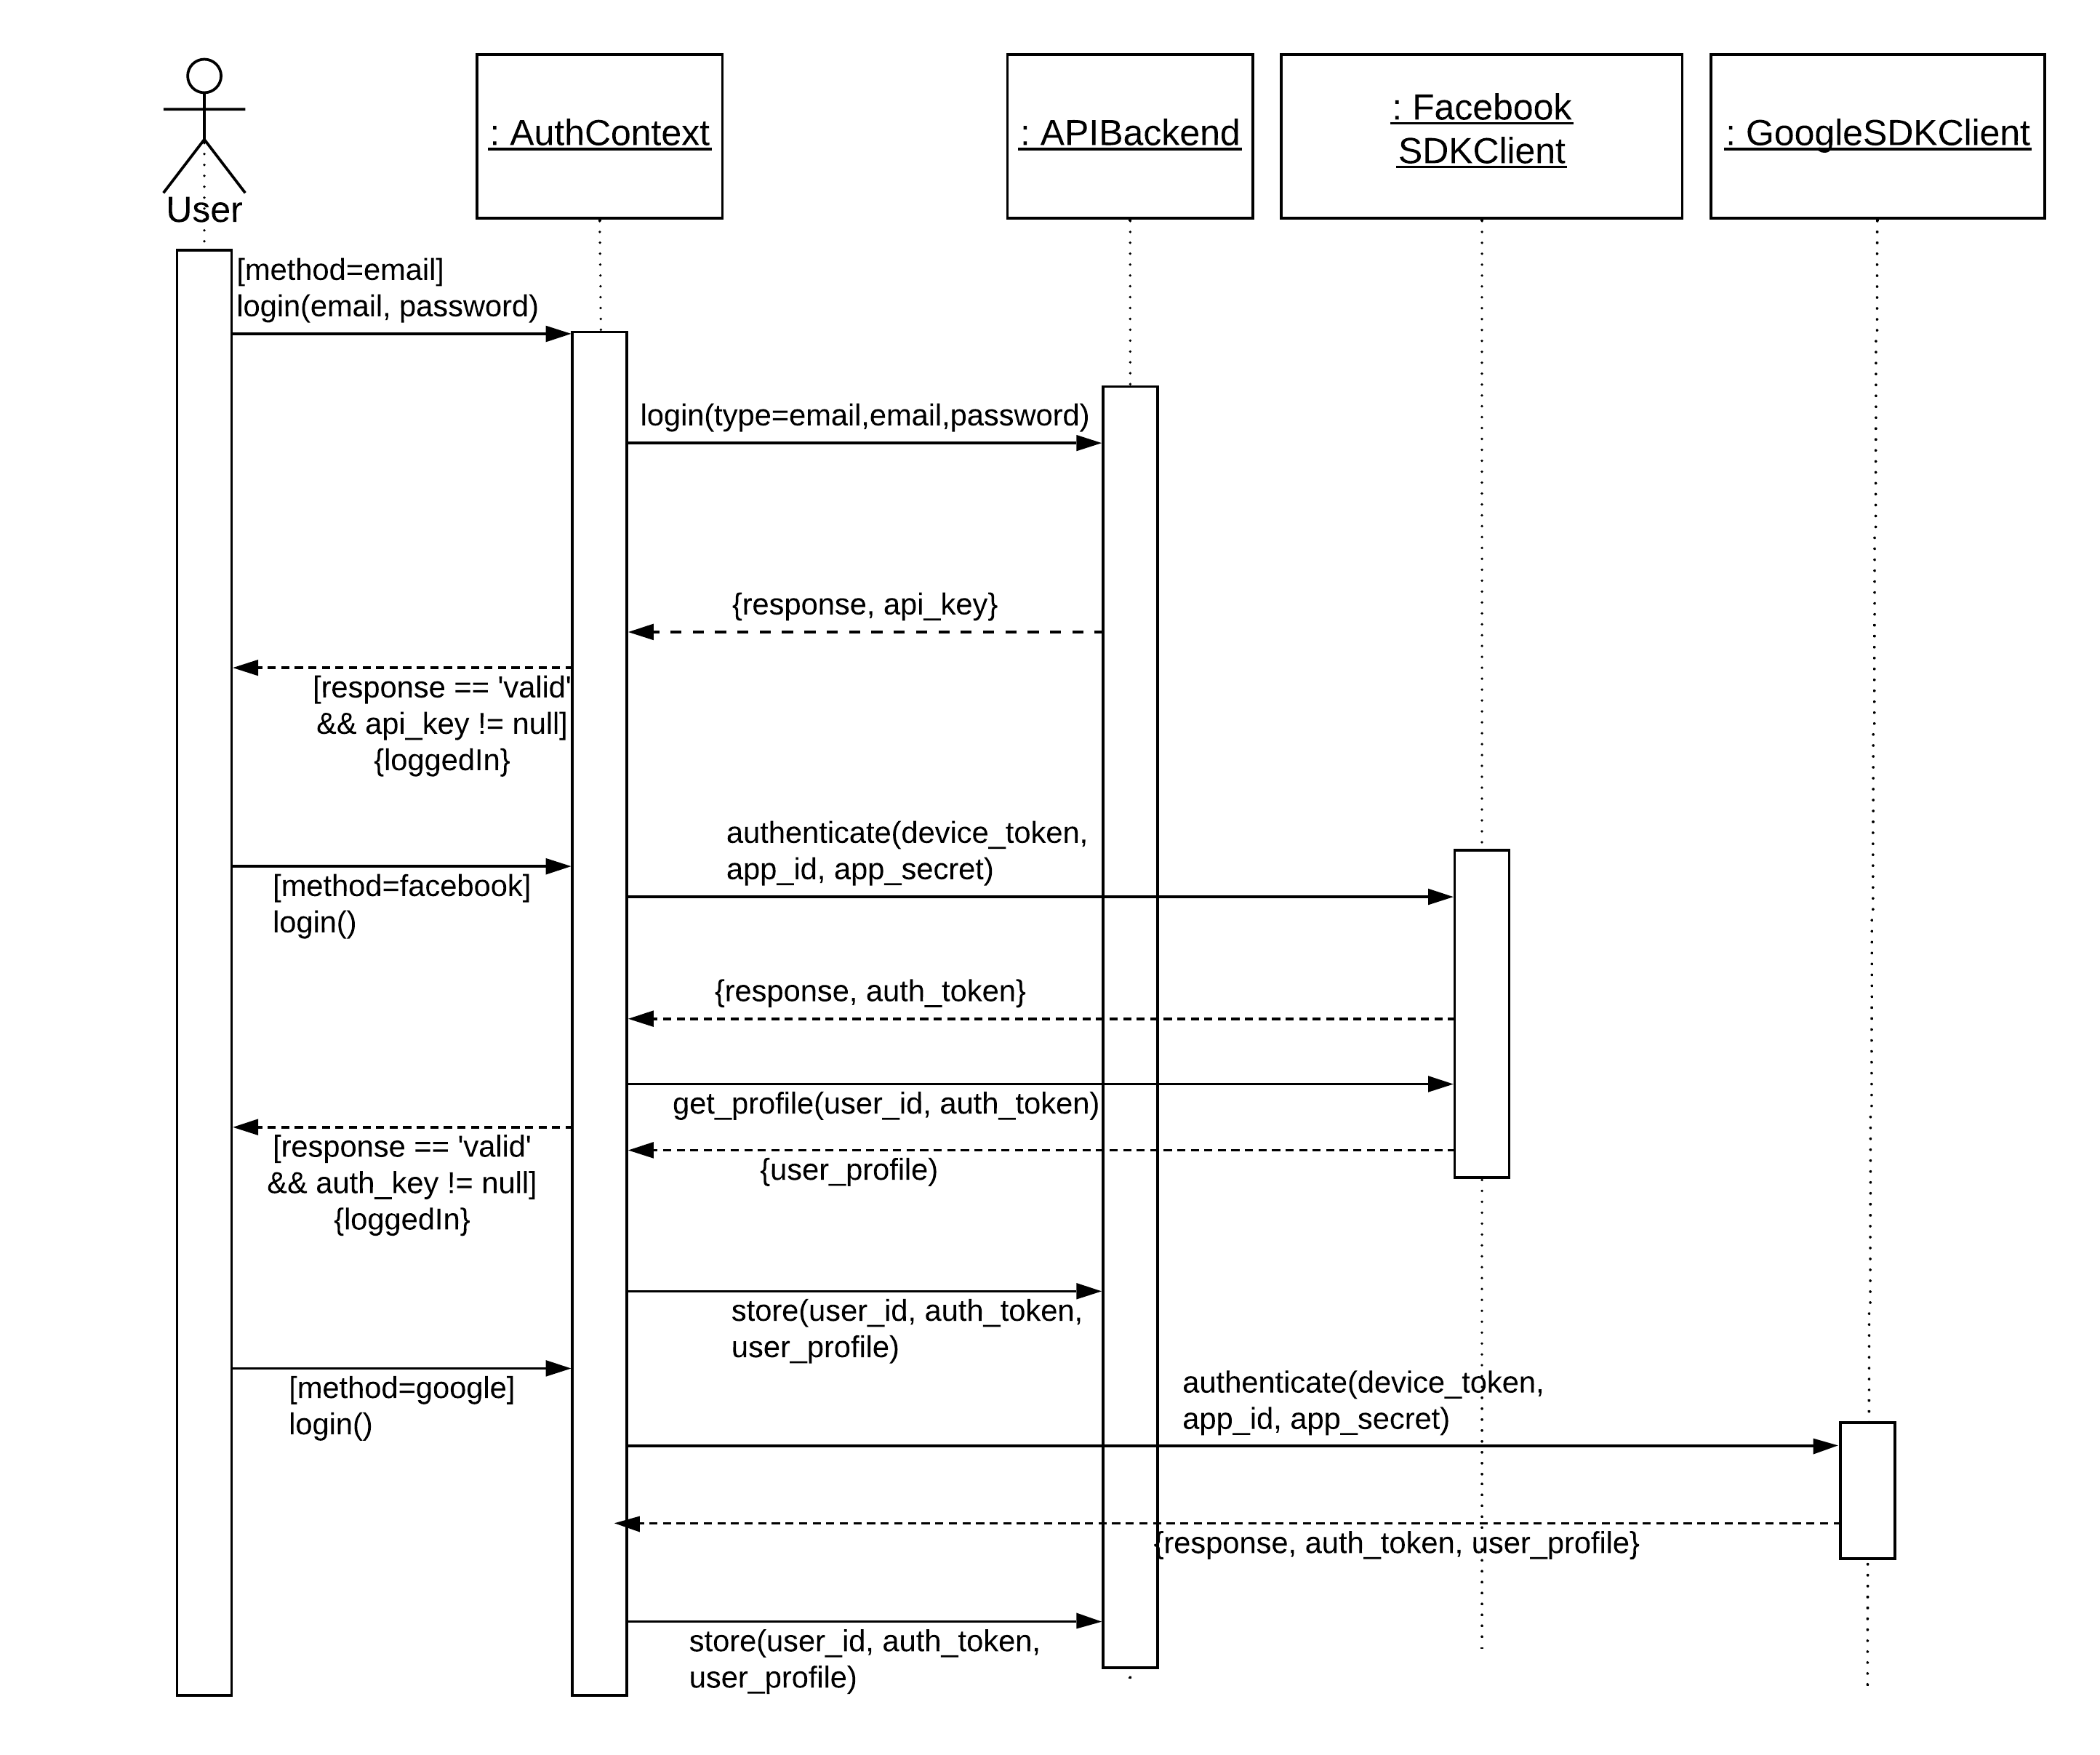
\includegraphics[width=\linewidth, keepaspectratio]{sequence-diagrams/login.png}
\centering
\caption{Sequence diagram for user authentication}
\label{fig:auth-sequence}
\end{figure}

\begin{figure}[H]
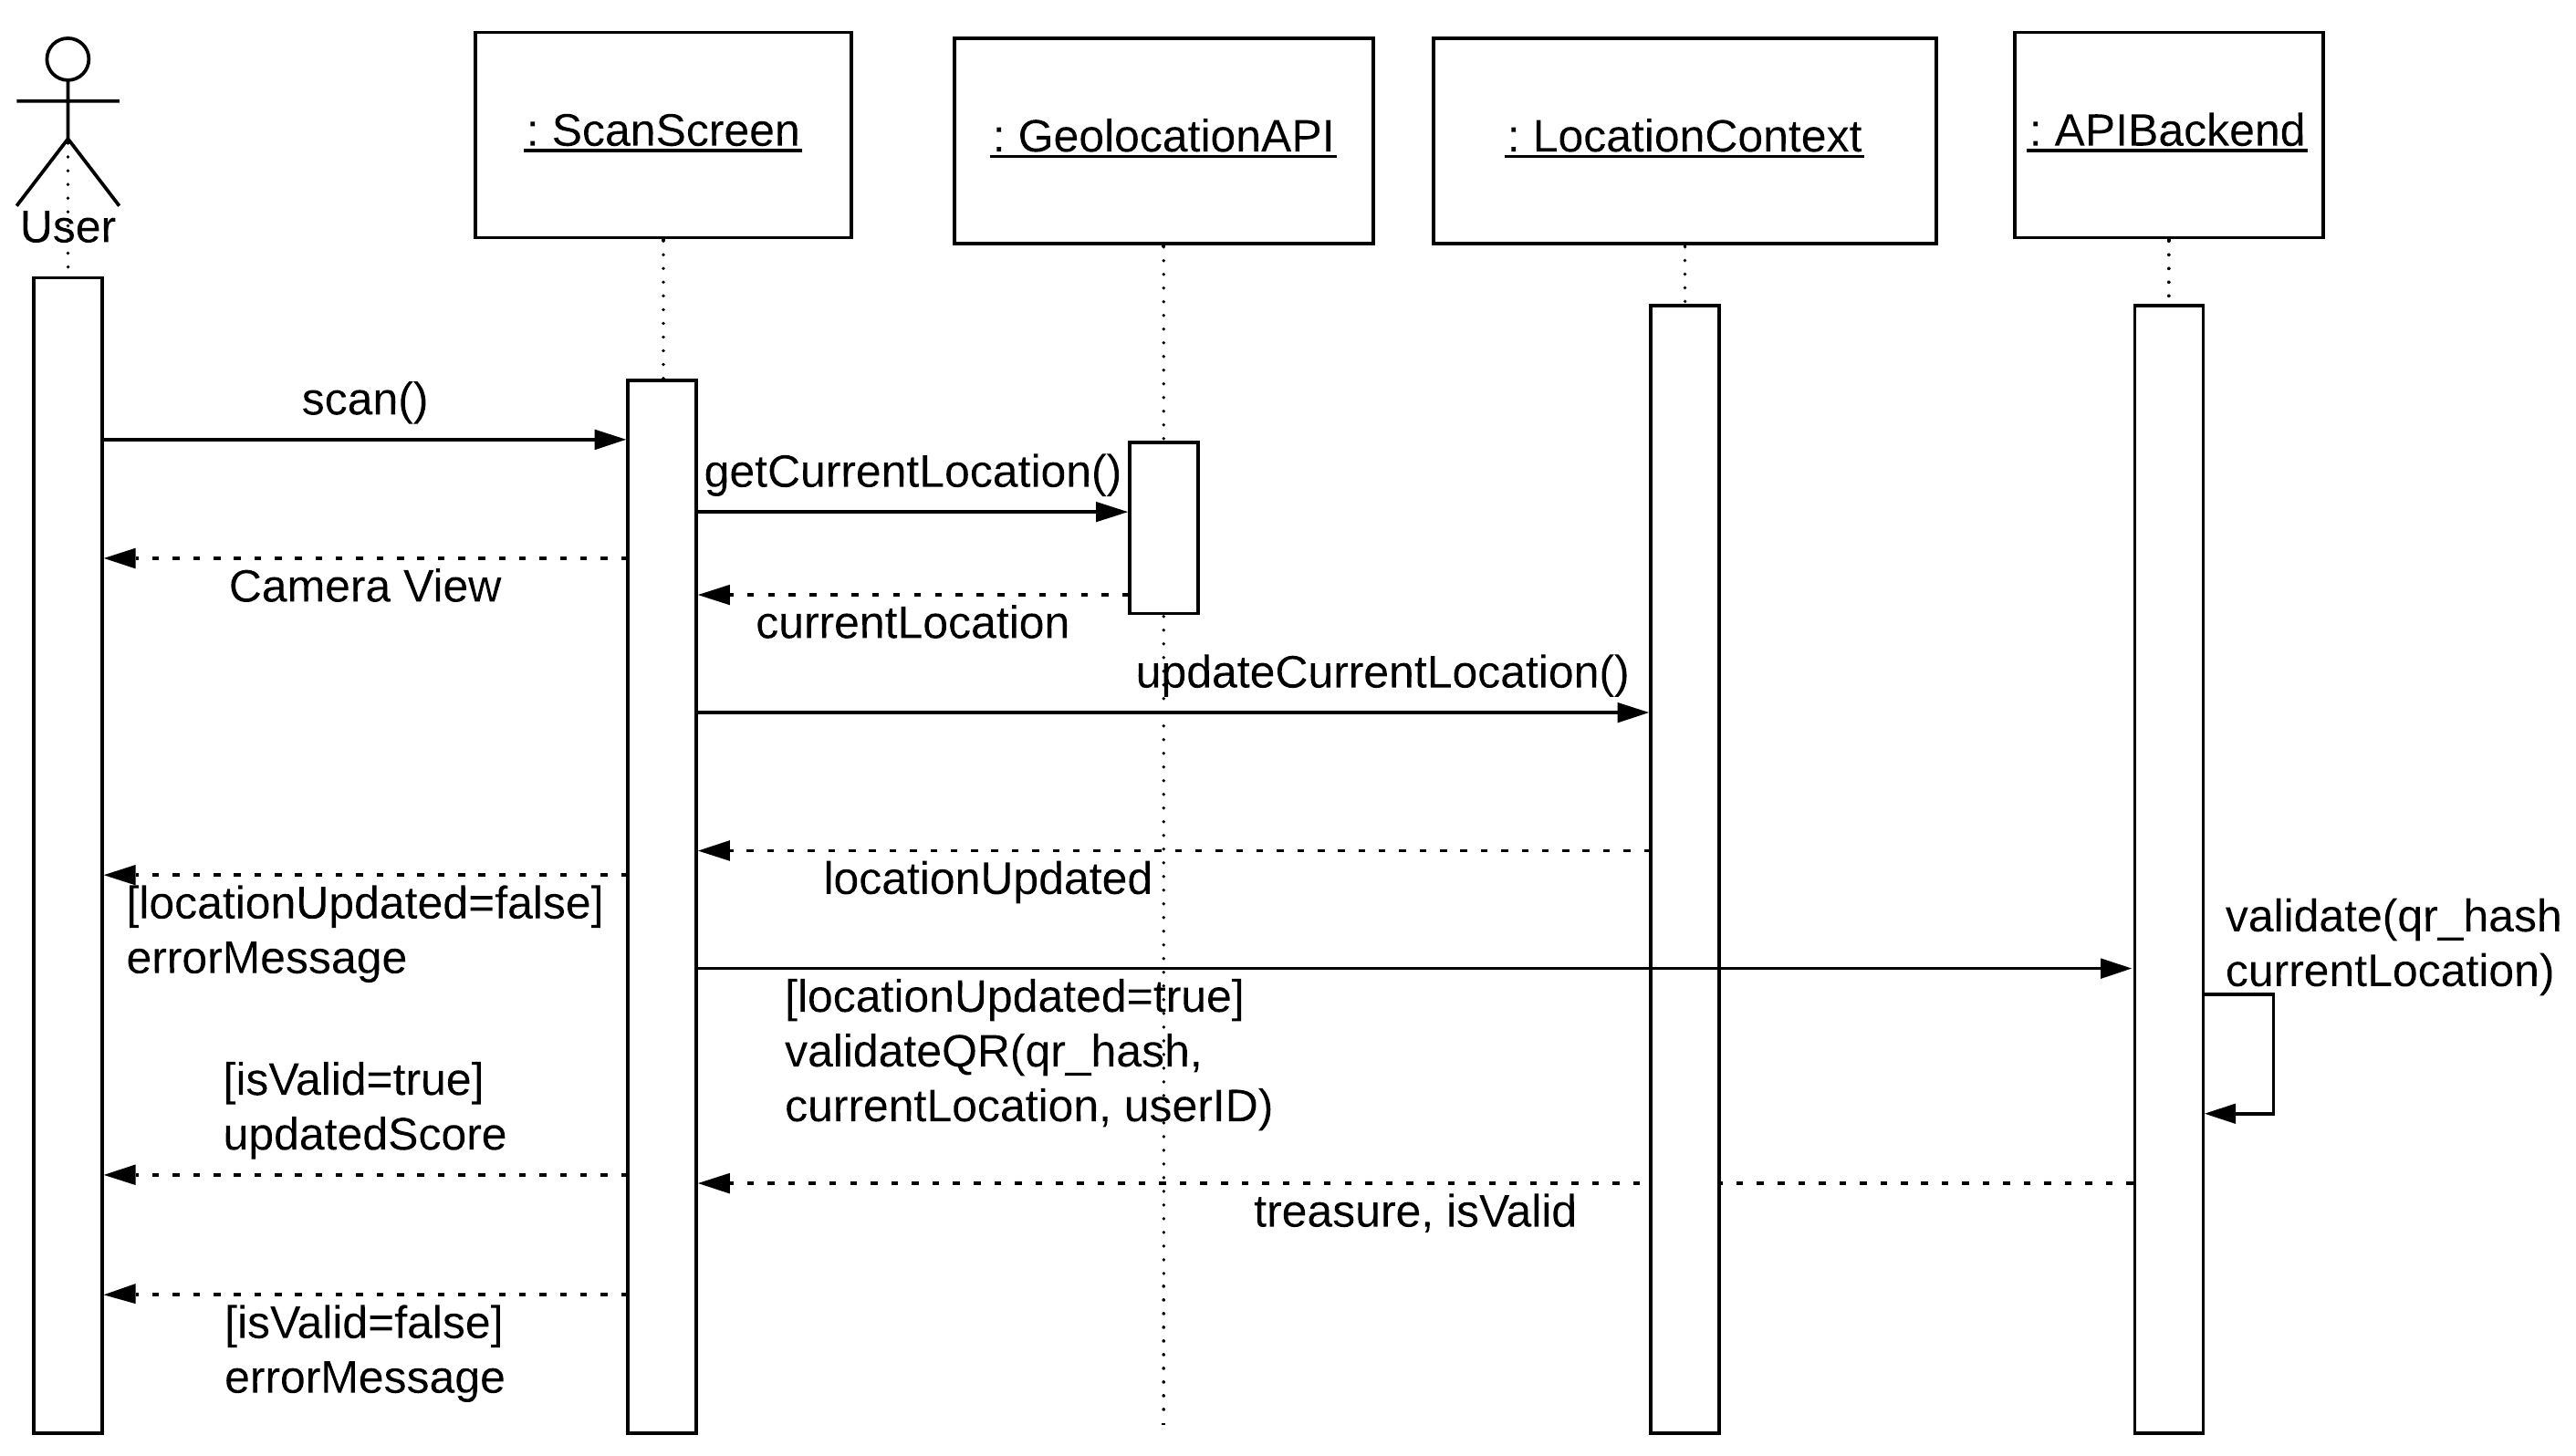
\includegraphics[width=\linewidth, keepaspectratio]{sequence-diagrams/treasure-scan.png}
\centering
\caption{Sequence diagram for treasure scanning}
\label{fig:treasure-scan-sequence}
\end{figure}

\begin{figure}[H]
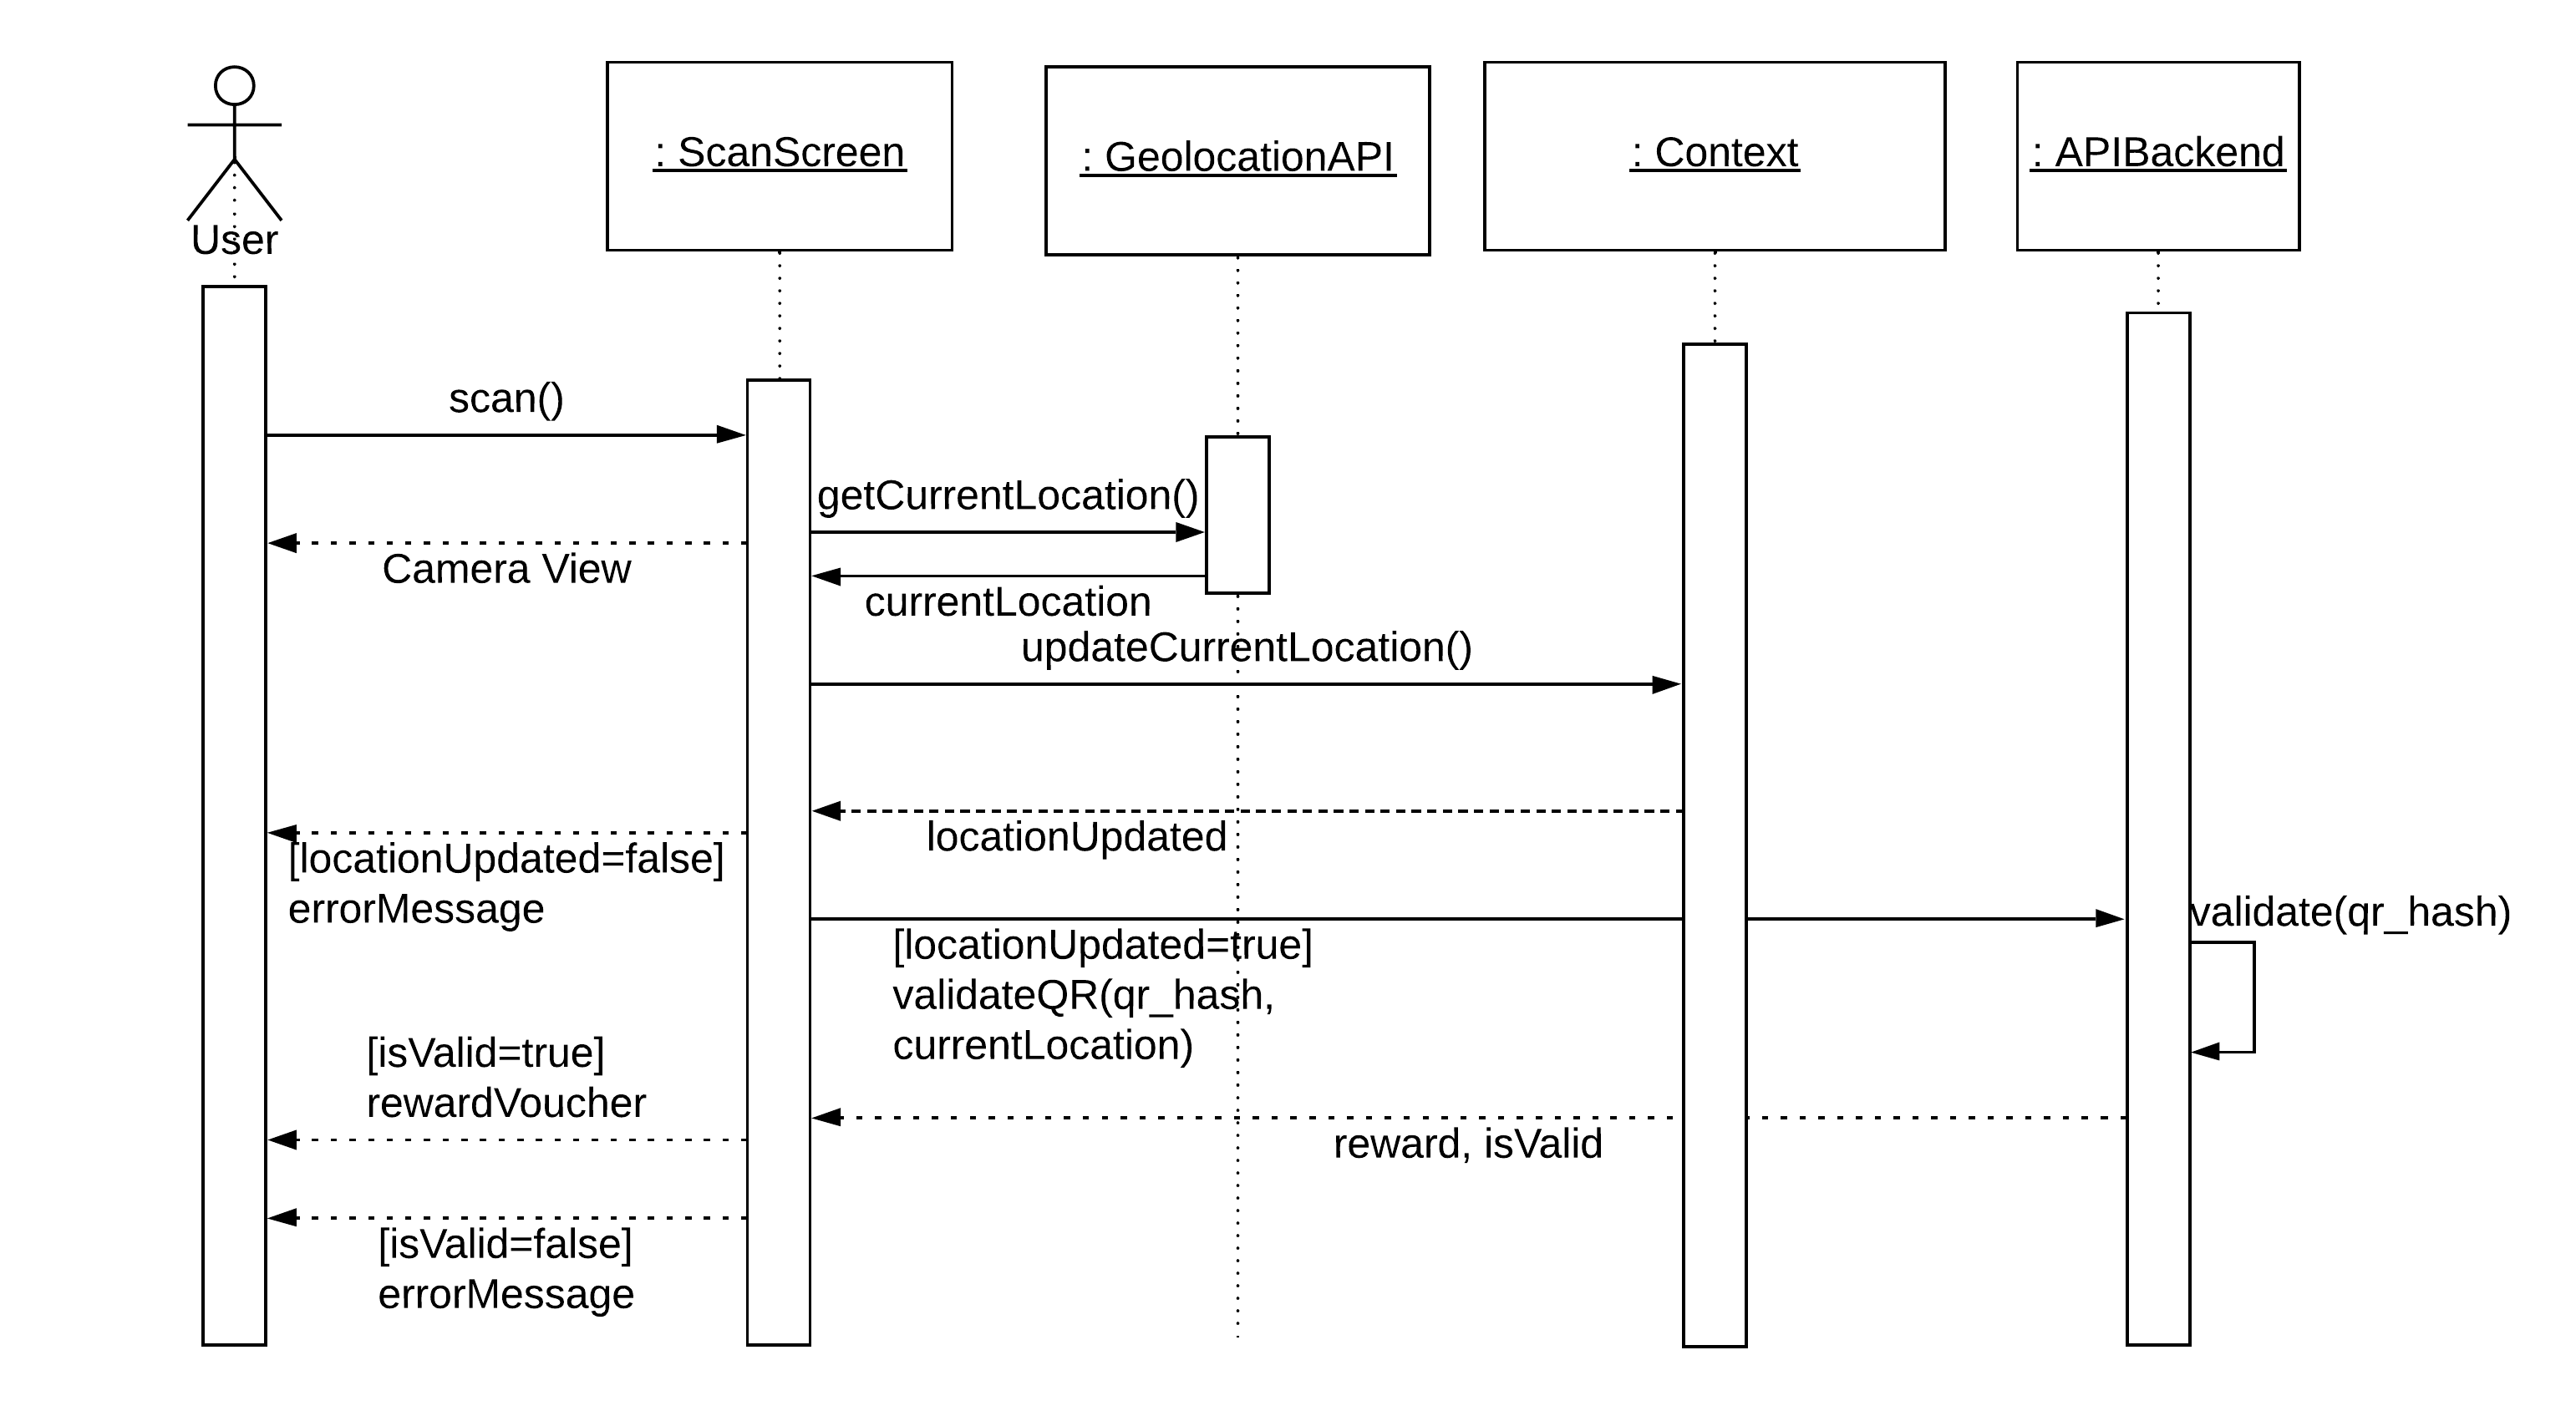
\includegraphics[width=\linewidth, keepaspectratio]{sequence-diagrams/reward-scan.png}
\centering
\caption{Sequence diagram for reward scanning}
\label{fig:reward-scan-sequence}
\end{figure}

\begin{figure}[H]
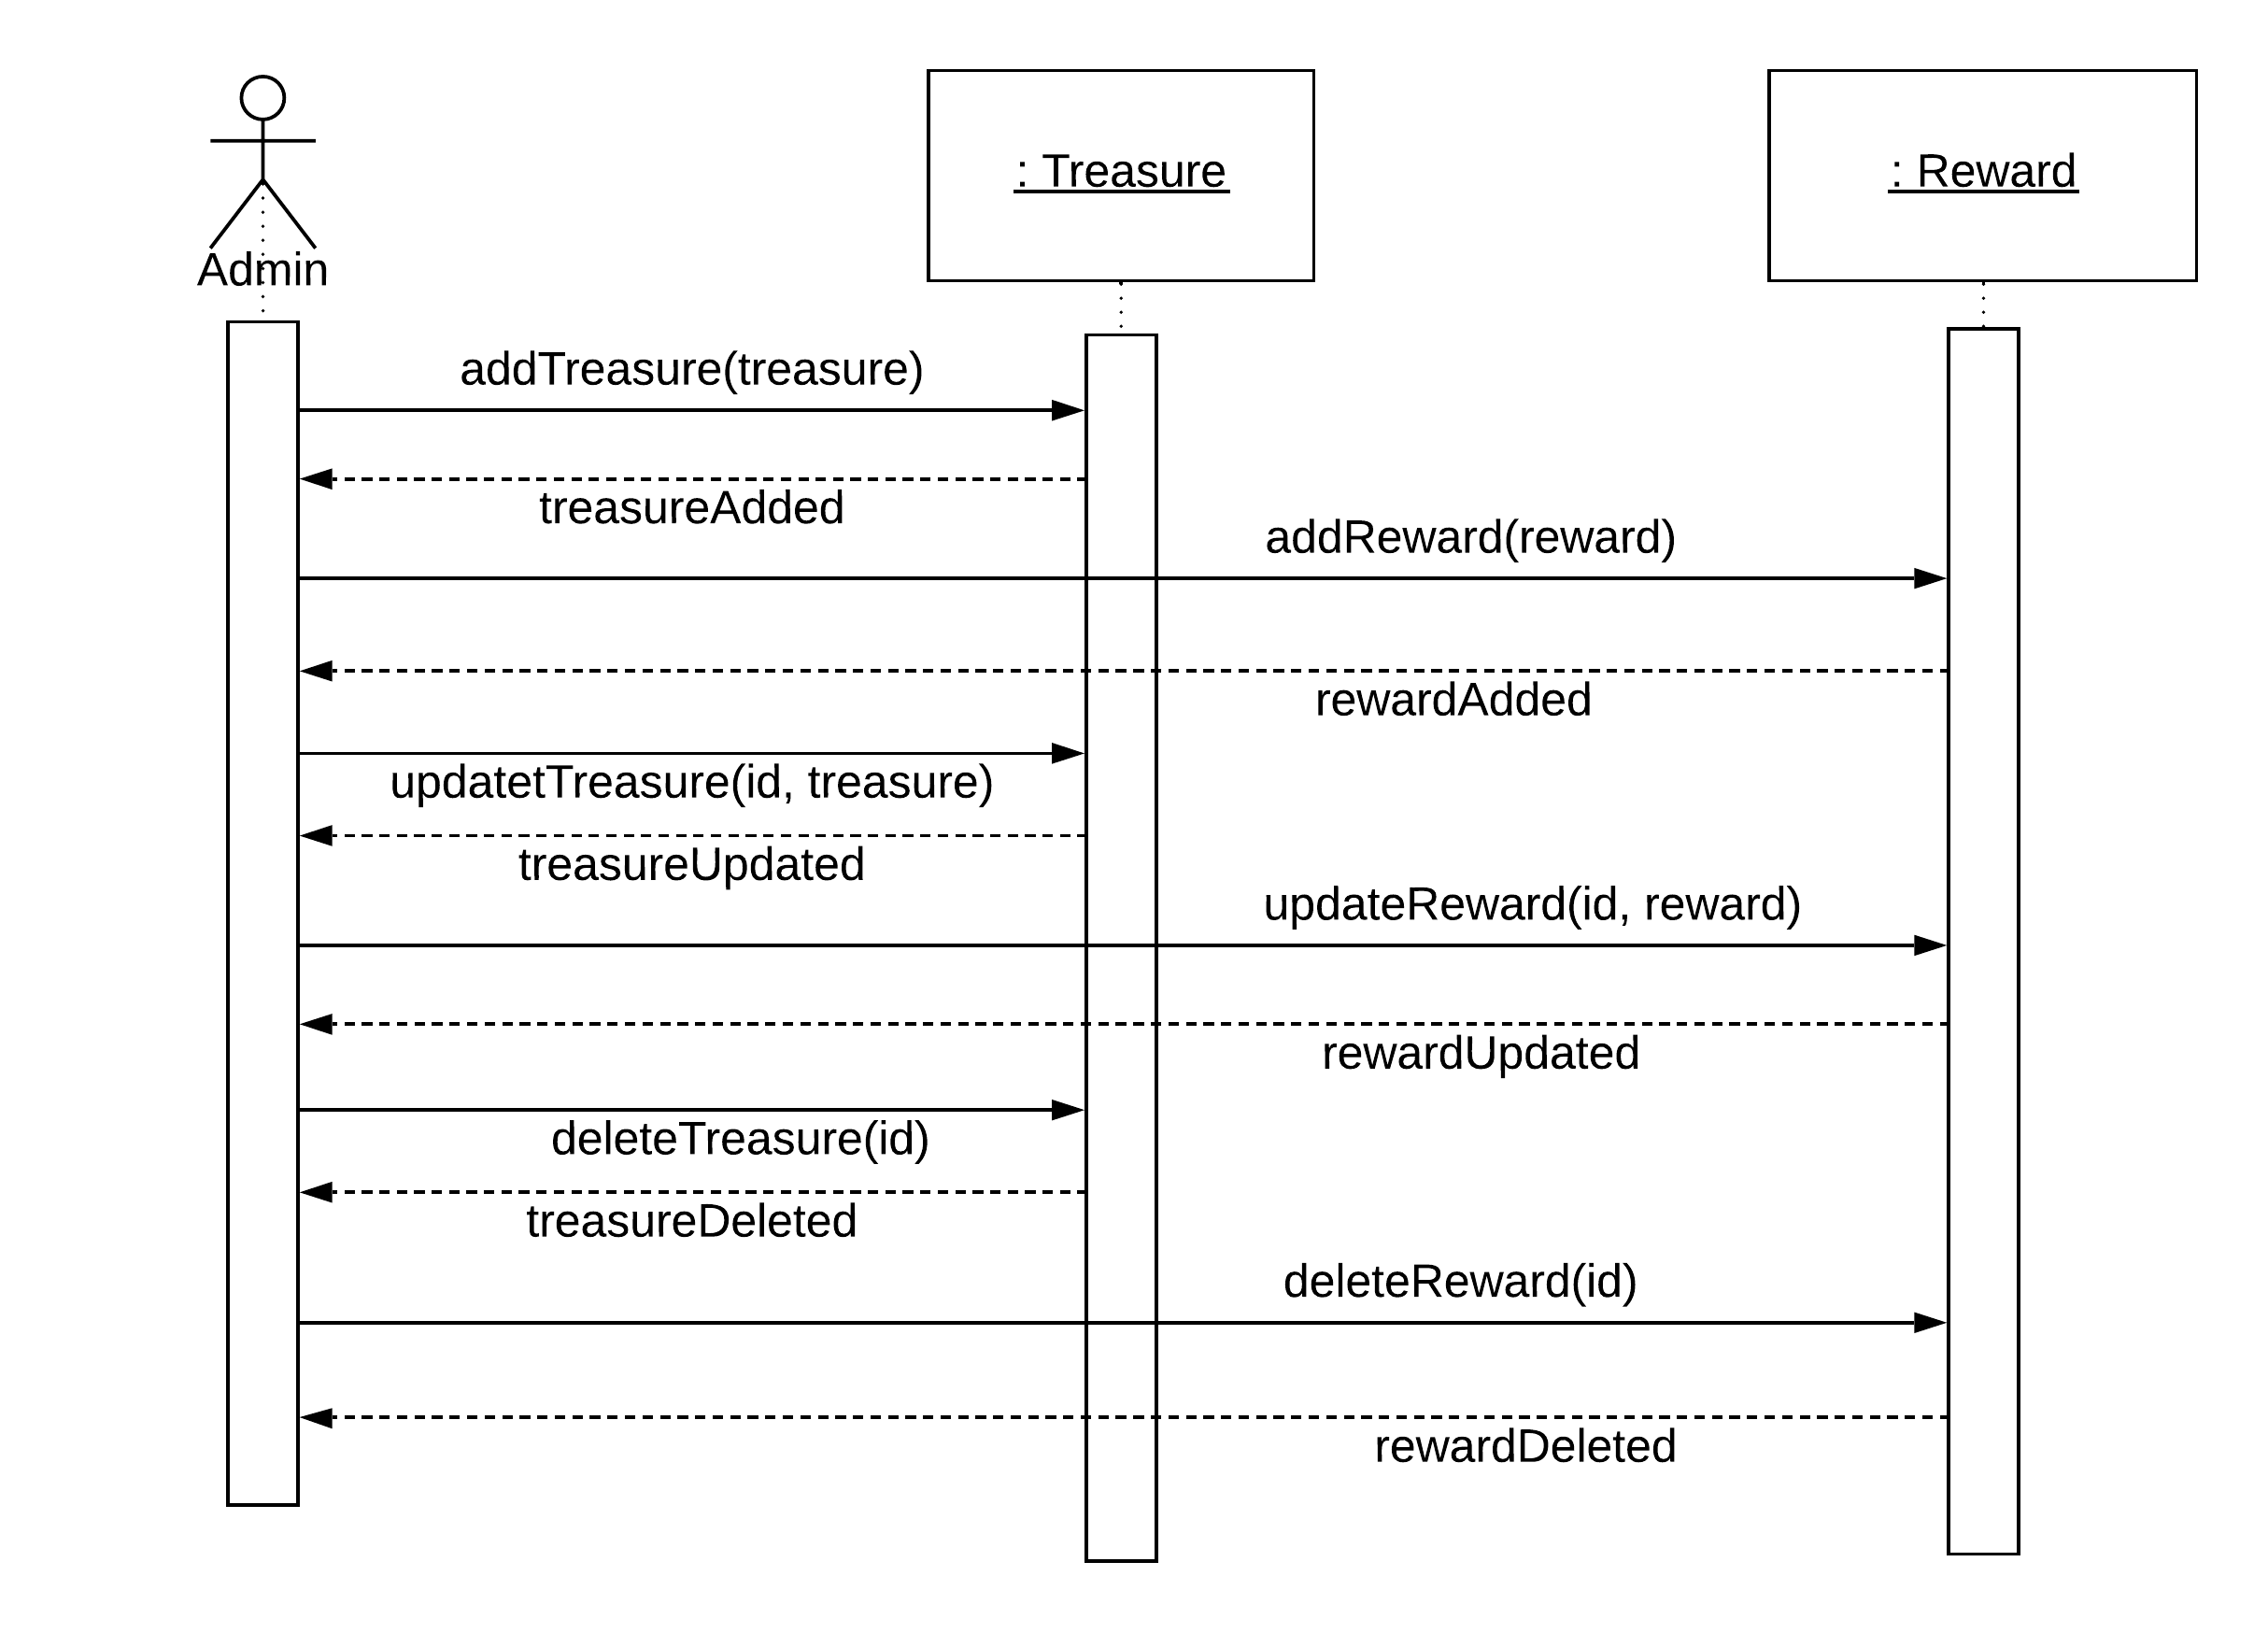
\includegraphics[width=\linewidth, keepaspectratio]{sequence-diagrams/admin-operations.png}
\centering
\caption{Sequence diagram for admin operations}
\label{fig:admin-operations-sequence}
\end{figure}

\pagebreak
\section{Coding and Implementation}
The coding and implementation phase starts after the complete high-level design of the system as per the SRS document. In this phase, the abstract designs developed during the design phase are actually implemented by the use of algorithms and then those algorithms are implemented in code using some programming language and frameworks. This section describes how we coded and implemented the various modules discussed in earlier sections of the document.

\subsection{API Development}
The backend API was developed using Python language in Django REST Framework. Django uses the famous Model View Controller (MVC) architecture. MVC architecture allows programmers to separate the data components and structures from the user interface. The models are the classes responsible for holding the data. The views are the classes responsible for rendering interface to the users. The controllers are the classes that act as a messenger between he models and views. For authentication, django-rest-auth library was used. Figure \ref{fig:backend-ide} shows the screenshot of development environment used for backend development.

\begin{figure}[H]
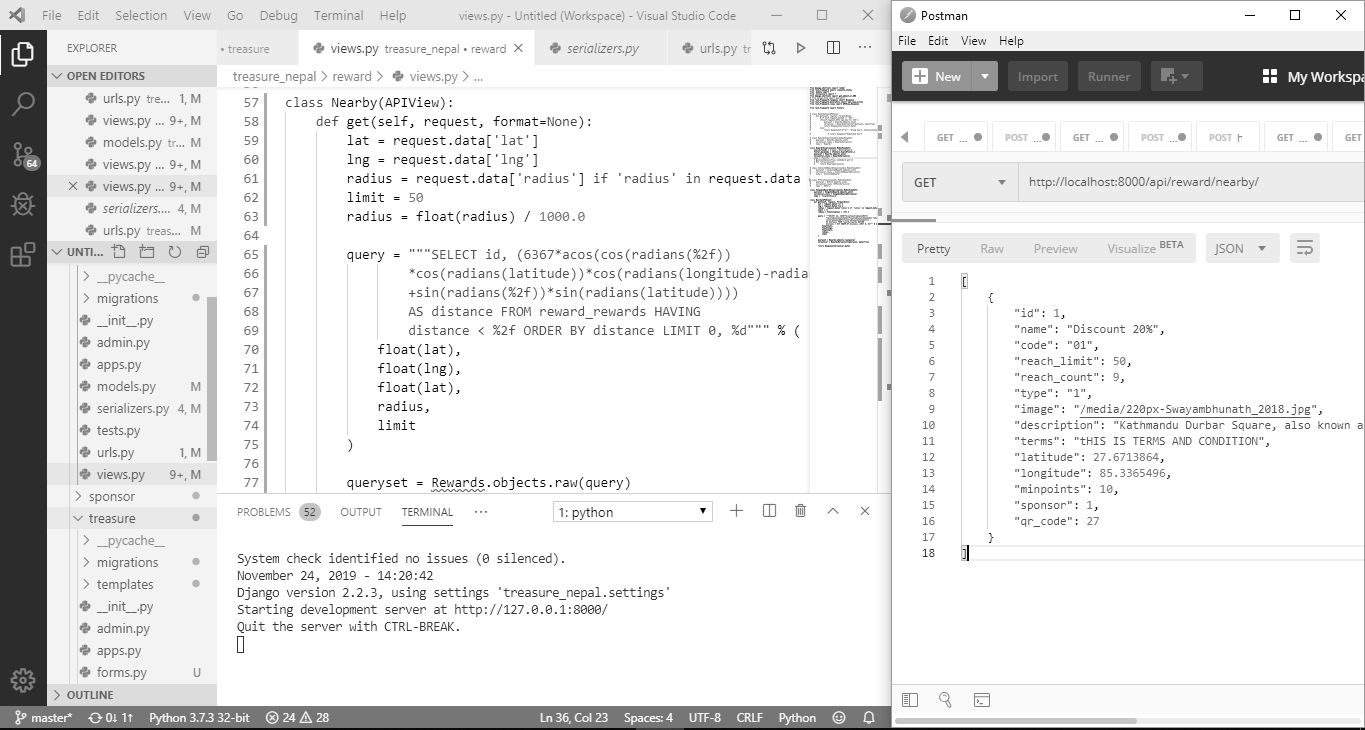
\includegraphics[width=\linewidth, keepaspectratio]{ide/backend.png}
\centering
\caption{Development environment of backend development}
\label{fig:backend-ide}
\end{figure}

\subsection{Mobile Application Development}
The frontend part of the project was done in React Native framework. Using react native framework enabled us to develop both android and iOS application with the same code base. For the state management in the front end application, we used the Redux library. The version of redux we used was called Redux Persistent, because it was modified in such a way that the data stored in state were persisted across multiple sessions of the application by writing them to the local storage. Figure \ref{fig:frontend-ide} shows the screenshot of developmen environmentt used for frontend development.

\begin{figure}[H]
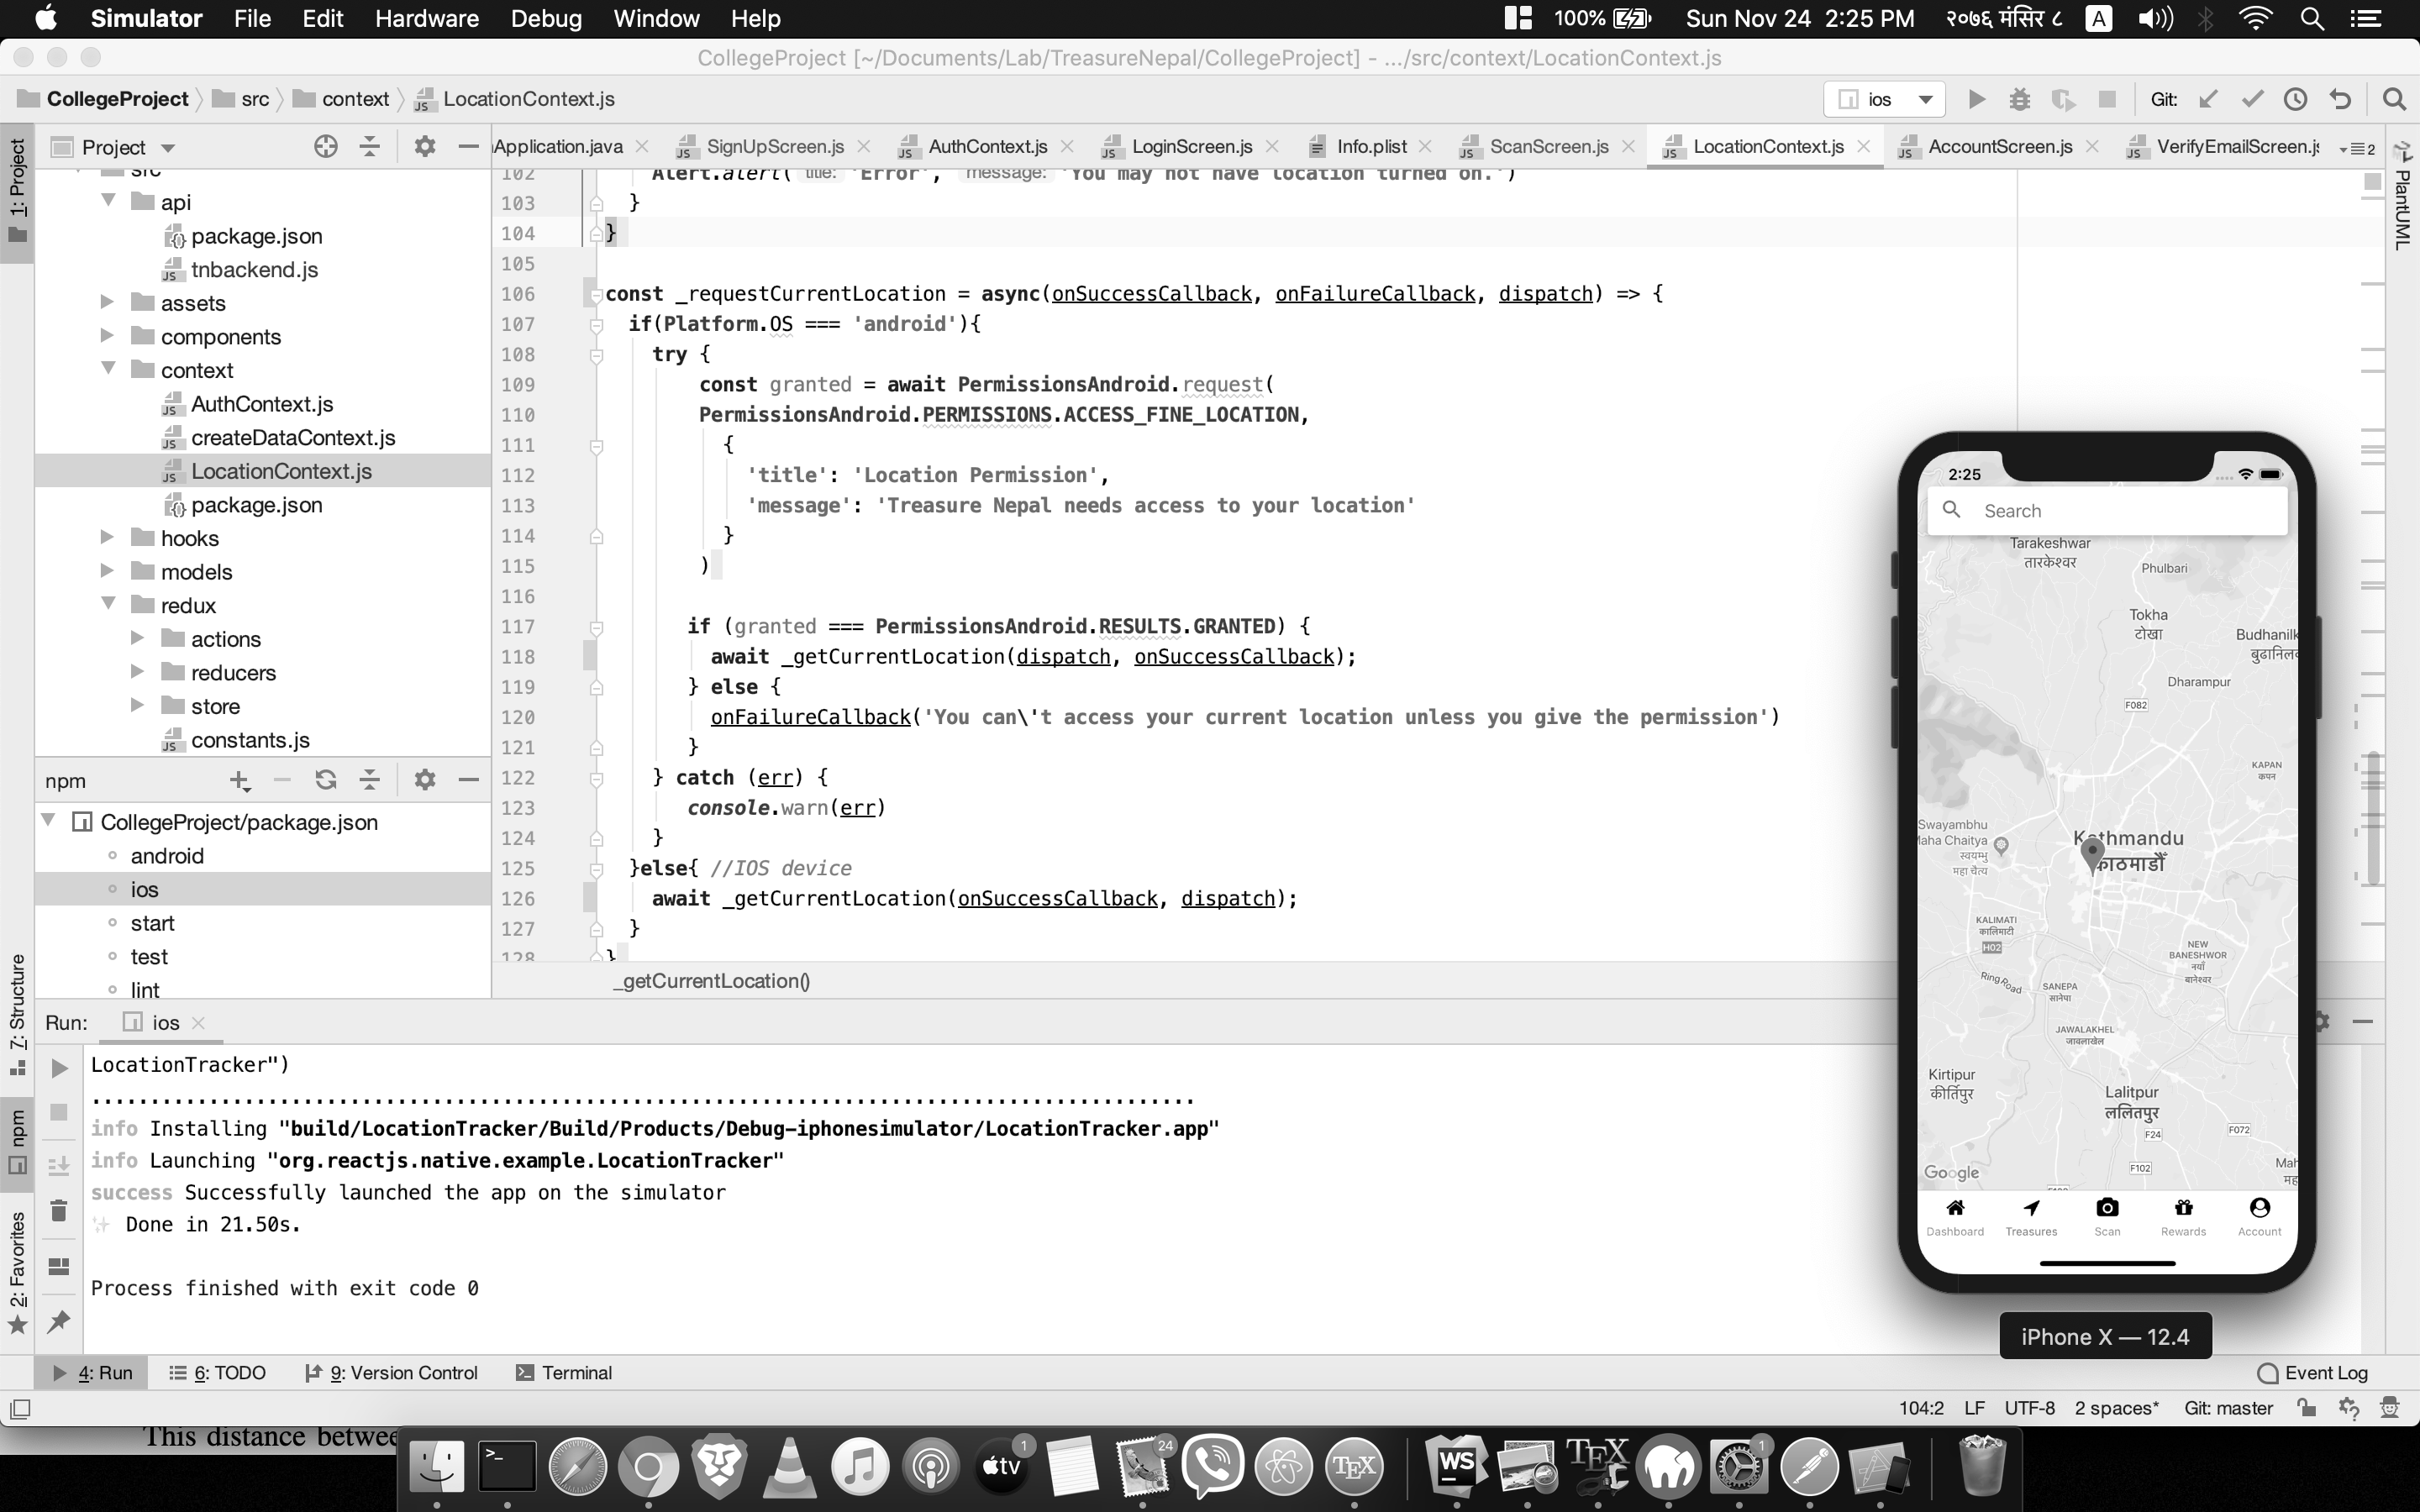
\includegraphics[width=\linewidth, keepaspectratio]{ide/frontend.png}
\centering
\caption{Development environment of Frontend development}
\label{fig:frontend-ide}
\end{figure}

\subsection{Algorithms}
We used a few popular algorithms in our project, some of which are described in the subsections that follow.

\subsubsection{Haversine Distance Calculation Algorithm}
Haversine formula, mentioned in equation \ref{eq:haversine} in subsection \ref{latlng} is a popular formula for calculating the great-circle distance between two points in the surface of a sphere. If the earth is considered as a sphere, the great-circle distance between the two points is the actual shortest distance from one place to another along the surface of the earth. This distance between the two points can be used to test whether the user is in the vicinity of the treasure location when he/she scans the QR code. Figure \ref{fig:haversine-python} shows how this algorithm can be implemented in python to validate whether a treasure scan is valid or not.

\lstset{language=Python,breaklines=true,frame=tb} 
\begin{figure}[H]
\begin{lstlisting}
import math

#Radius of the earth (approx) in meters
RADIUS = 6371000

def hav(a):
  return math.sin(a/2) ** 2

#returns distance between two points in meters
def distance(lat1, long1, lat2, long2):
  lat1_rad = lat1 * math.pi/180
  lat2_rad = lat2 * math.pi/180
  long1_rad = long1 * math.pi/180
  long2_rad = long2 * math.pi/180
  h = hav(lat2_rad - lat1_rad) + math.cos(lat2_rad)*math.cos(lat1_rad)*hav(long2_rad-long1_rad)
  return 2*RADIUS*math.asin(math.sqrt(h))

def validate(treasure, current_location):
  d = distance(treasure.latitude, treasure.longitude, current_location.latitude, current_location.longitude)
  return True if d <= treasure.permitted_distance else False
\end{lstlisting}
\caption{Python implementation of haversine formula}
\label{fig:haversine-python}
\end{figure}

As an example let us consider that there is a treasure installed at Balkumari Temple, Lalitpur. The coordinates of Balkumari Temple are $(A_1, B_1) = (27.671971, 85.335900)$. Now let that a tourist scans the QR code of the treasure at Balkumari temple sitting at the Nepal College of Information Technology. The coordinates of NCIT are $(A_2, B_2) = (27.671359, 85.338801)$. Now, by equation \ref{eq:haversine}, the distance between Balkumari Temple and NCIT is given by:

\begin{math}
A_1 = 27.671971^0 = 0.482967\ rad \\
A_2 = 27.671359^0 = 0.482956\ rad\\
B_1 = 85.335900^0 = 1.489392\ rad\\
B_2 = 85.338801^0 = 1.489443\ rad\\
H_A = \sin^2 \left( \frac{ 0.482956 - 0.482967}{2} \right) = 3.025 \times 10^{-11} \\
H_B = \sin^2 \left( \frac{1.489443 - 1.489392}{2} \right) = 6.5025 \times 10^{-10} \\
d = 2 \times 6371000 \times \sin^{-1} \left( \sqrt { H_A + \cos{0.482967} \cos{0.482956} H_B } \right) = 293.67 m
\end{math}

This means that, if the treasure installed at Balkumari Temple has permitted distance of scan more than 293.67 meters, the tourist will be able to collect that treasure from Nepal College of IT, whereas if it is less than 293.67 meters, the tourist will not be able to collect that treasure from NCIT. He/She should move closer to the treasure in order to collect it.

%\subsection{Backend API}
%The API endpoints for creating, updating, reading and deleting the data from all of the tables shown in Figure \ref{fig:db-schema} have already been created. The following table shows the syntax of different endpoints of the API.
%
%\begin{table}[H]
%\begin{tabularx}{\linewidth}{|c|c|c|X|}
%\hline
%\rowcolor[HTML]{C0C0C0} 
%\textbf{Endpoint}                & \textbf{Method} & \textbf{Body}        & \textbf{Response}                                               \\ \hline
%/\{table\_name\}        & GET    & -           & List of all data entries in the table                  \\ \hline
%/\{table\_name\}/\{id\} & GET    & -           & The entry in the table corresponding to provided ID    \\ \hline
%/\{table\_name\}/       & POST   & data object & Entry for data object created in the database          \\ \hline
%/\{table\_name\}/\{id\} & PUT    & data object & Update the entry with provided id with new data object \\ \hline
%/\{table\_name\}/\{id\} & DELETE & -           & Delete the entry corresponding to the provided id      \\ \hline
%\end{tabularx}
%\end{table}
%
%The following figure shows an instance of API request and response.
%
%\begin{figure}[H]
%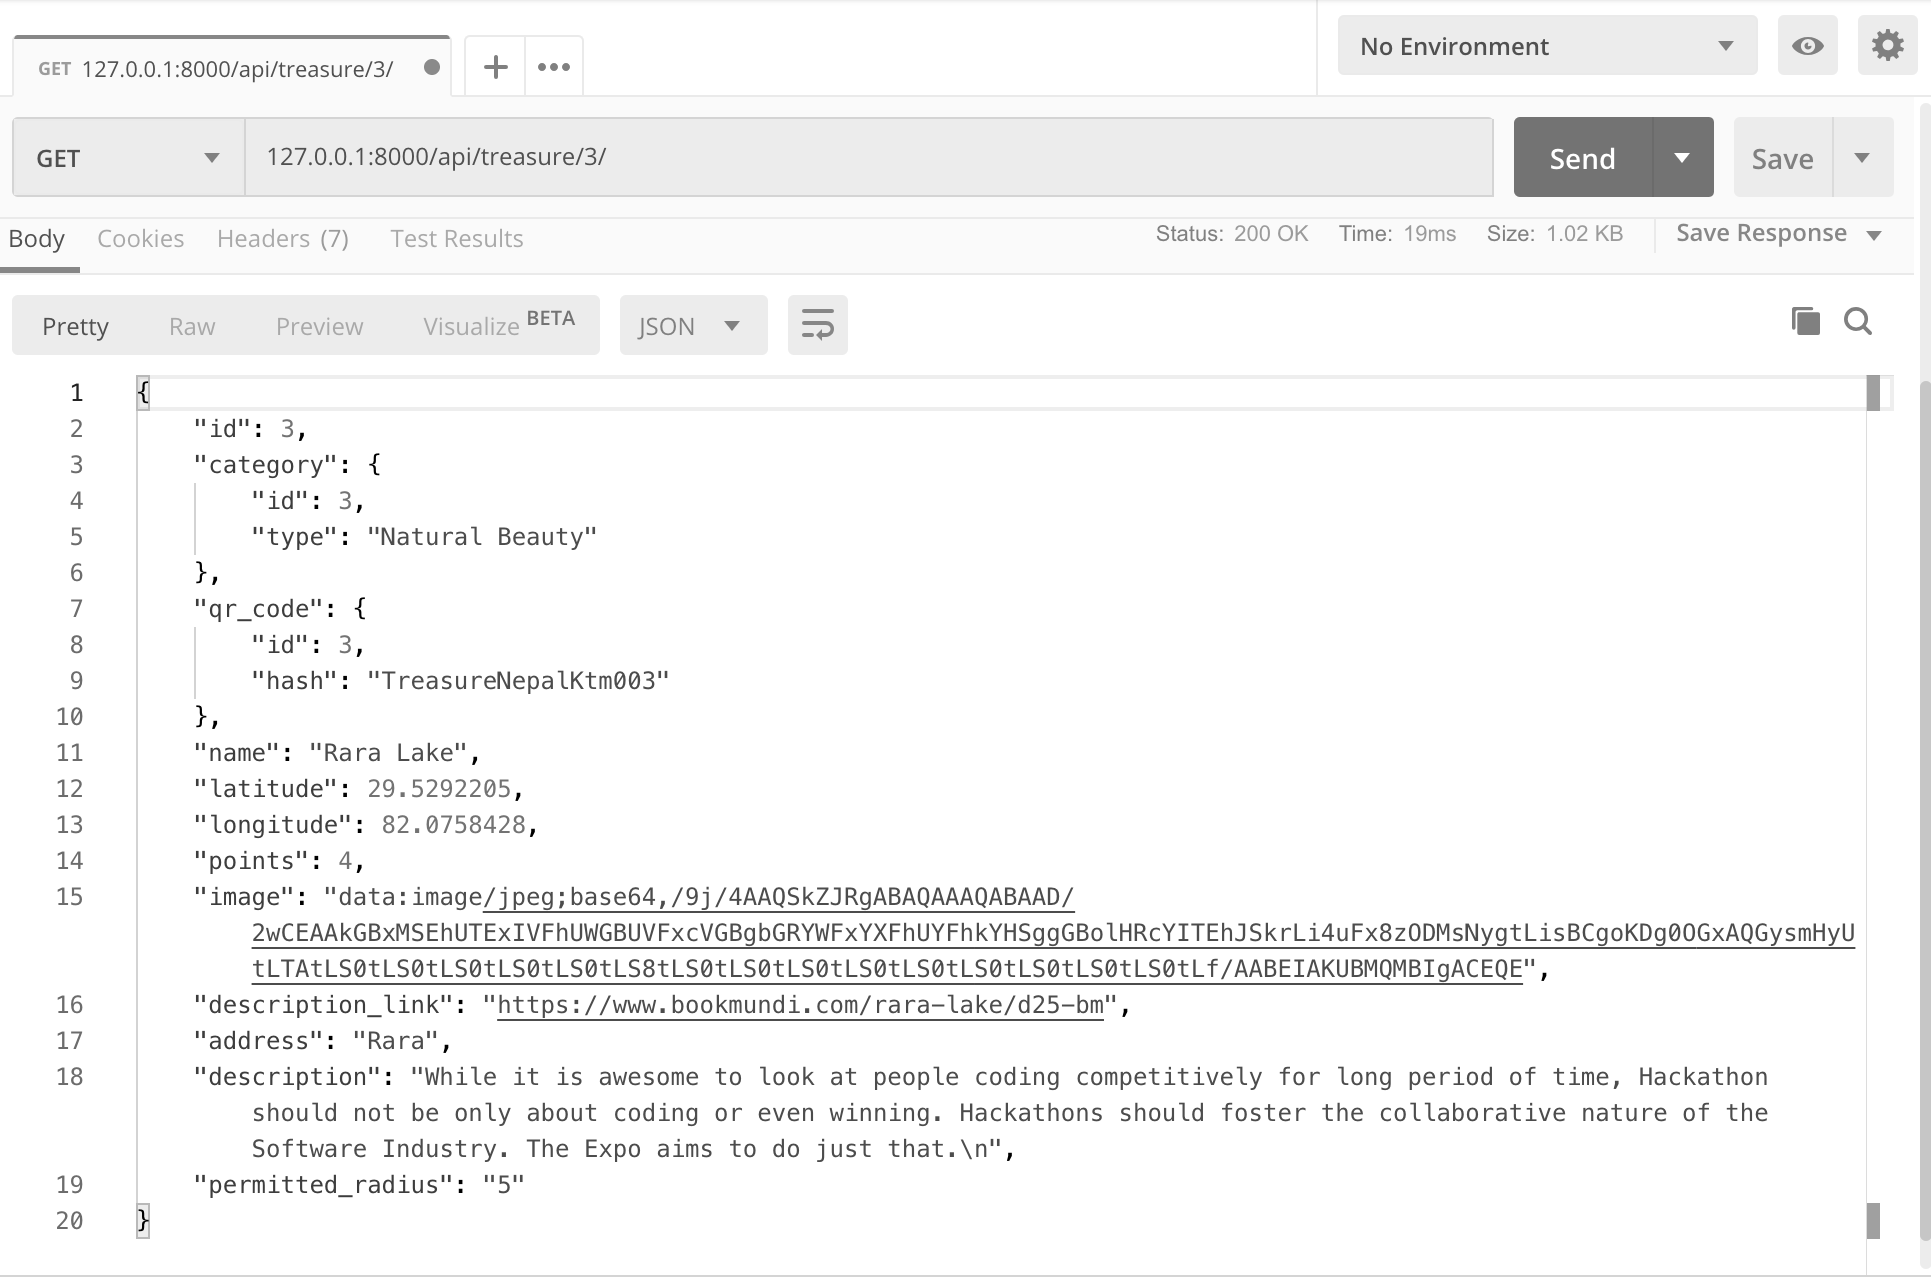
\includegraphics[width=\linewidth, keepaspectratio]{screenshots/api.png}
%\centering
%\caption{Screenshot of API request and response using Postman}
%\label{fig:auth-sequence}
%\end{figure}
%
%
%\subsection{Authentication Module}
%The user authentication module has been completed in the backend, using email, Facebook as well as Google. In the backend, we have use django-rest-auth module for authentication management. This gives the user a unique api key whenever she logs in to the application. The user should then include that key in every request she sends to the API server.
%
%
%
%\subsection{Application Development}
%The authentication has been integrated in the application development and as of now, it is fully working in both Android and iOS devices. The user can successfully login and out either using email, Facebook or Google sign in options.
%
%The following figures show some screenshots of the application developed so far.
%
%\begin{figure}[H]
%\centering
%	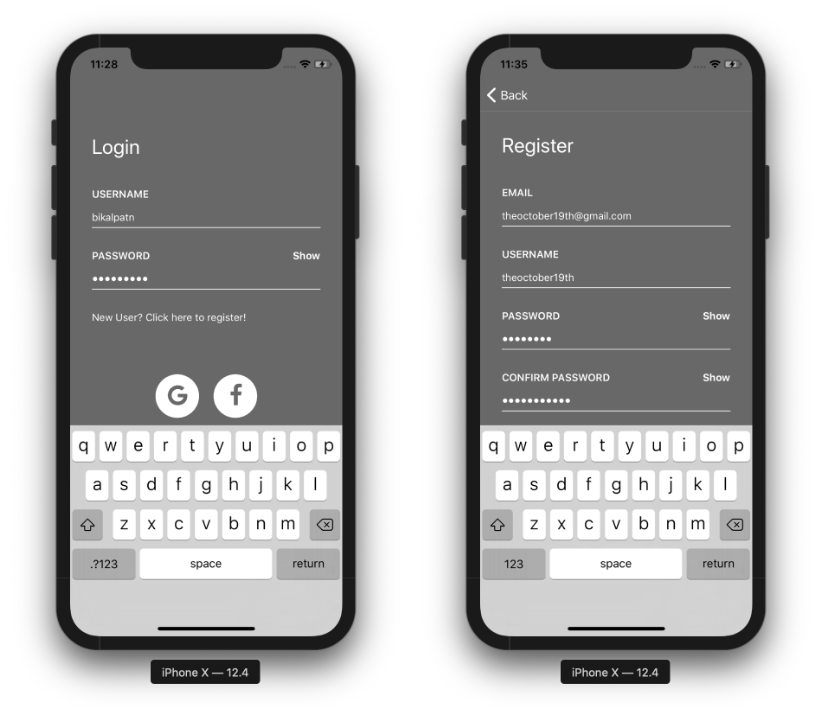
\includegraphics[width=\linewidth]{screenshots/1.png}	
%	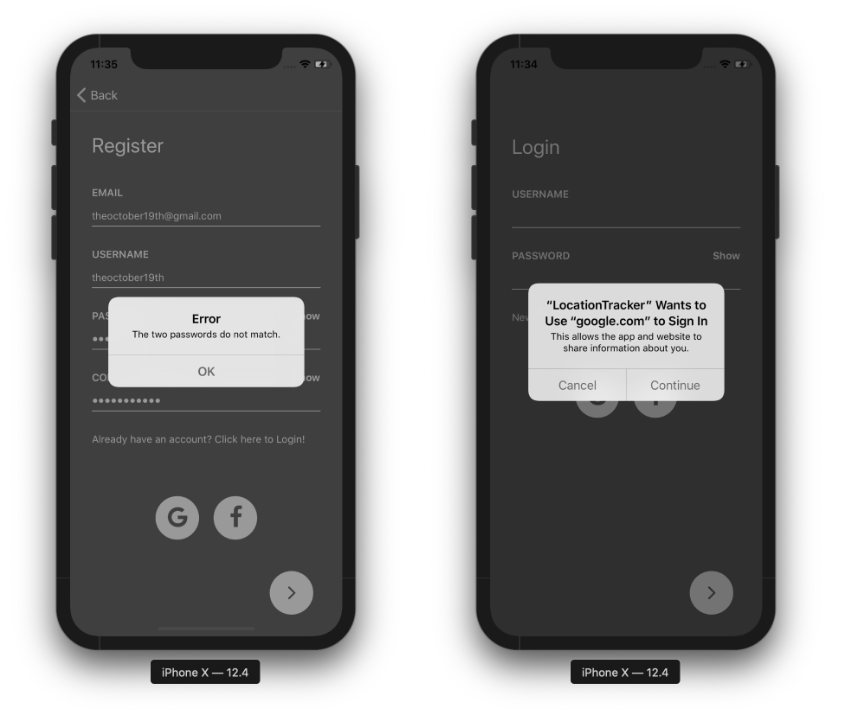
\includegraphics[width=\linewidth]{screenshots/2.png}	
%\end{figure}
%
%
%
%\begin{figure}[h]
%\centering
%	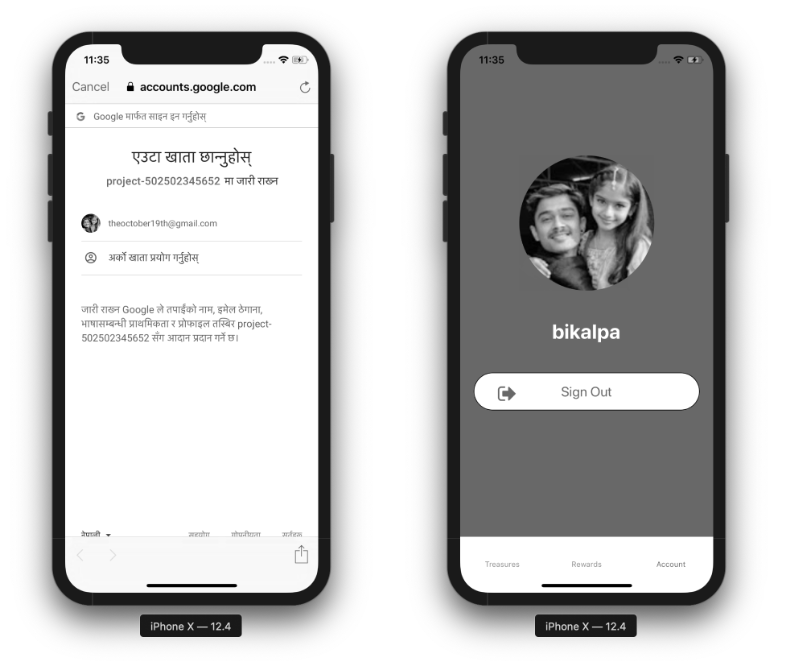
\includegraphics[width=\linewidth]{screenshots/3.png}
%	\caption{Screenshots of the application developed}
%	\label{fig:sc}	
%\end{figure}


\pagebreak
\section{Testing and Debugging}
After the coding and implementation phase is complete, it is customary that the features implemented be tested so that they fulfill exact requirements documented in SRS document. Our team conducted the unit testing of the different features of our application by preparing a set of unit test cases and compared the expected output with the actual output. Whenever the actual output came deviated from the expected output, we debugged the application to find the issue and correct it.

\subsection{Tools Used in Testing}
Due to the cost and resource limitation, the number of devices and tools used for testing the product is quite small. The devices and tools used for unit testing are listed in Table \ref{table:unit-test-devices}

\begin{table}[H]
\begin{tabularx}{\linewidth}{|c|X|X|}
\hline
\rowcolor[HTML]{C0C0C0} 
S.N. & Tool               & Specifications                                            \\ \hline
1.   & Android Smartphone & Manufacturer: Oneplus \newline Model: Oneplus2 \newline Android version: 9 \\ \hline
2.   & iOS Simulator      & Model: iPhone X \newline iOS version: 12.4                        \\ \hline
3.   & Postman            & Version 7.12.0                                           \\ \hline
\end{tabularx}
\caption{Tools and devices used in testing phase}
\end{table}

\subsection{Unit Test Cases} \label{testcases}
This section consists of various test cases, expected outcomes and actual outcomes during unit testing of the project.

\LTXtable{\linewidth}{tables/unit-test/auth-test.tex}
\pagebreak
\LTXtable{\linewidth}{tables/unit-test/treasure-test.tex}
\LTXtable{\linewidth}{tables/unit-test/reward-test.tex}

\subsection{Test Evidences}
This section consists of screenshots of various instances of the application as an evidence that the test cases mentioned in section \ref{testcases} were in fact passed successfully.

\begin{figure}[H]

\begin{subfigure}{.5\textwidth}
    \centering
    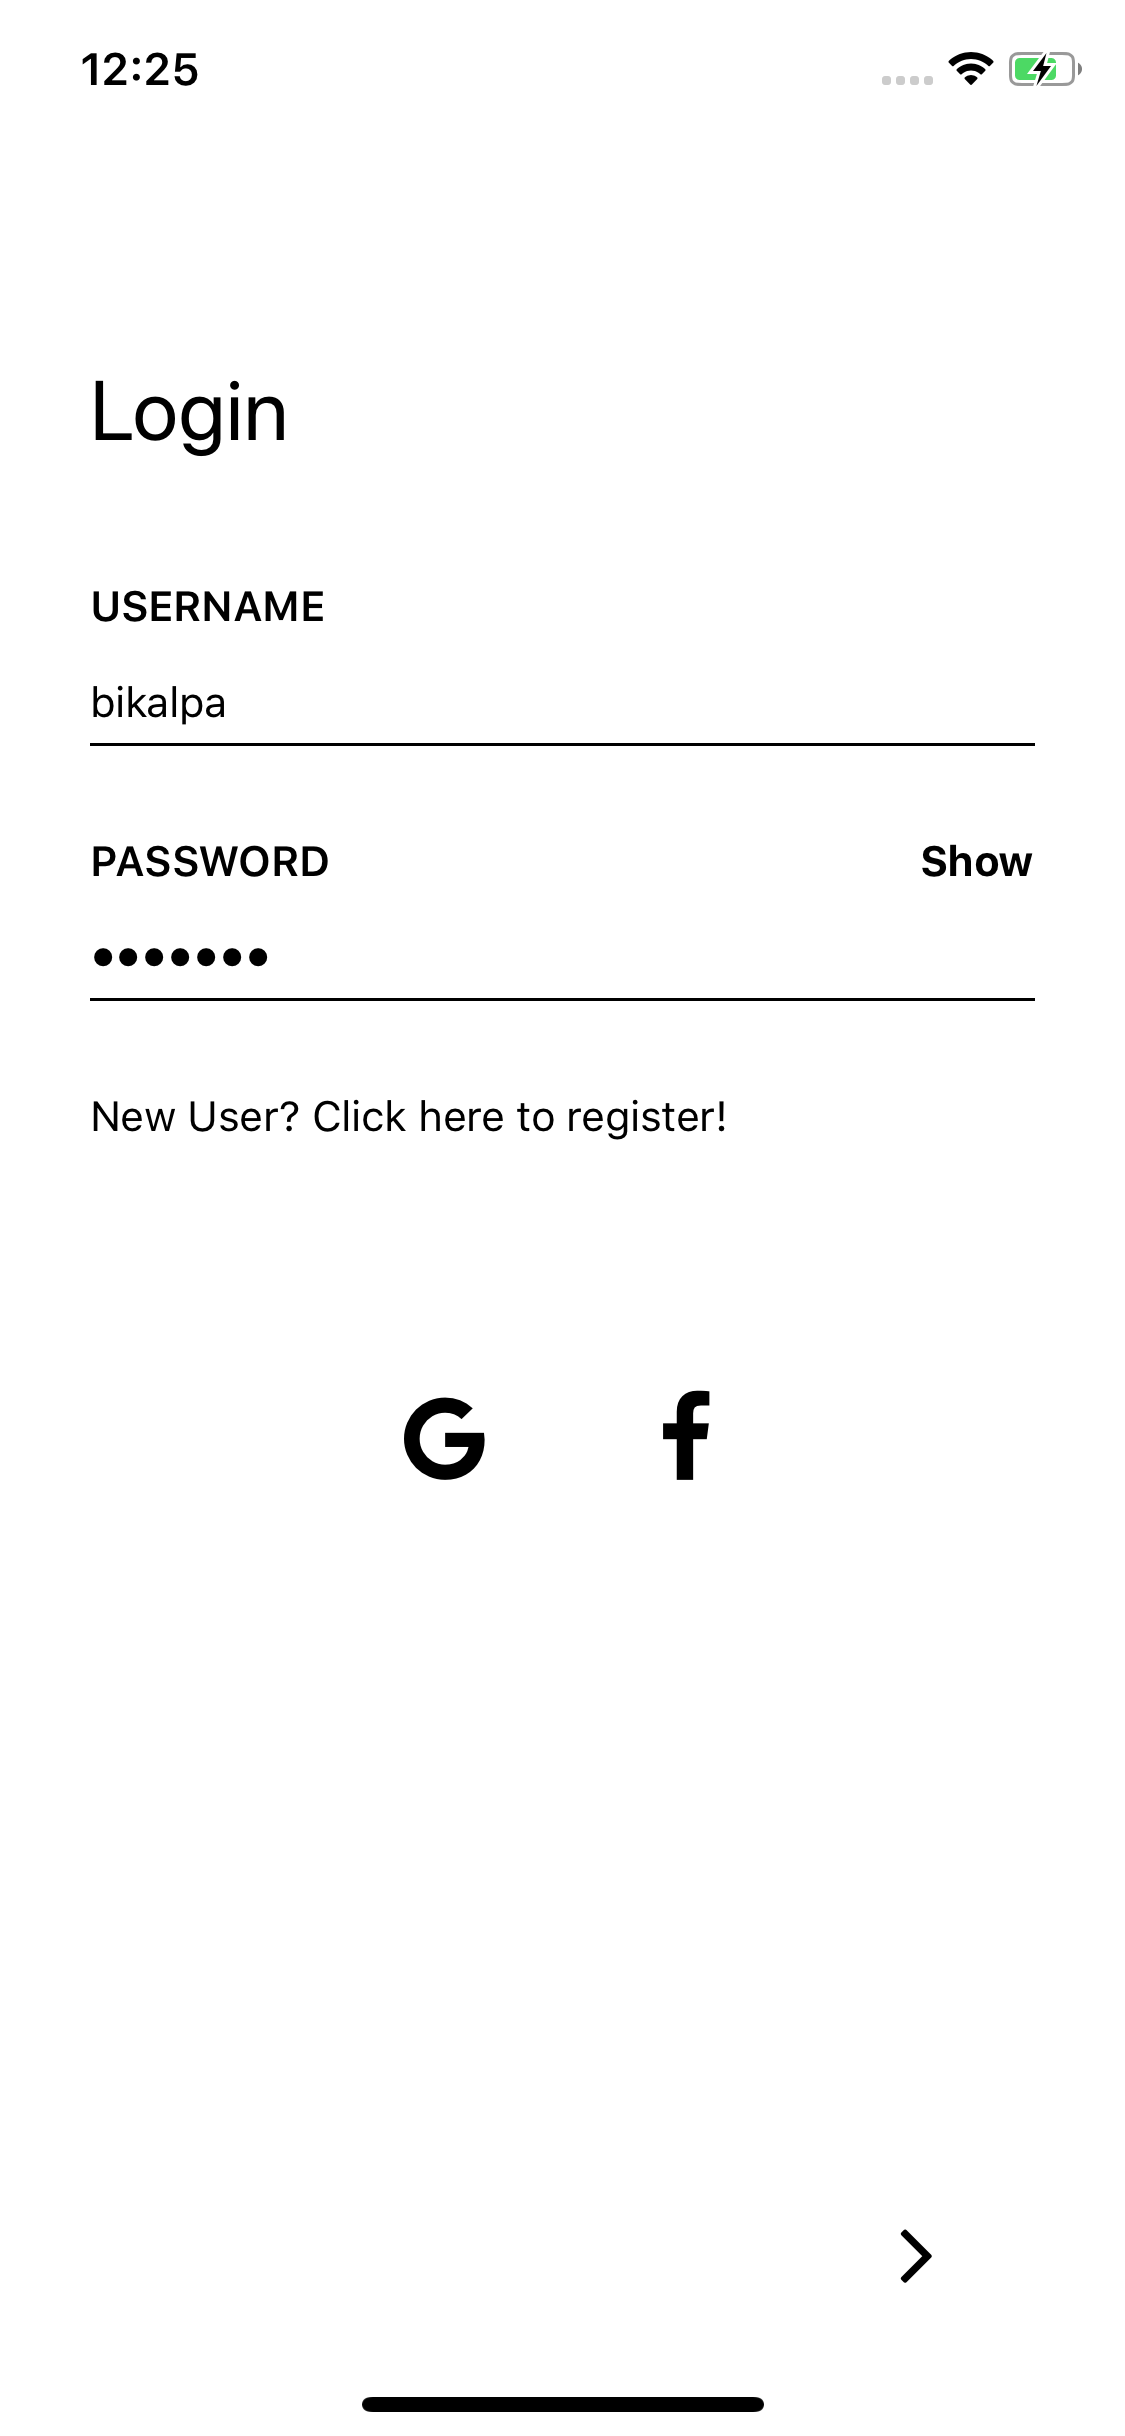
\includegraphics[width=0.45\textwidth]{test-evidences/auth/a.png}
    \caption{}
\end{subfigure}%
\begin{subfigure}{.5\textwidth}
    \centering
    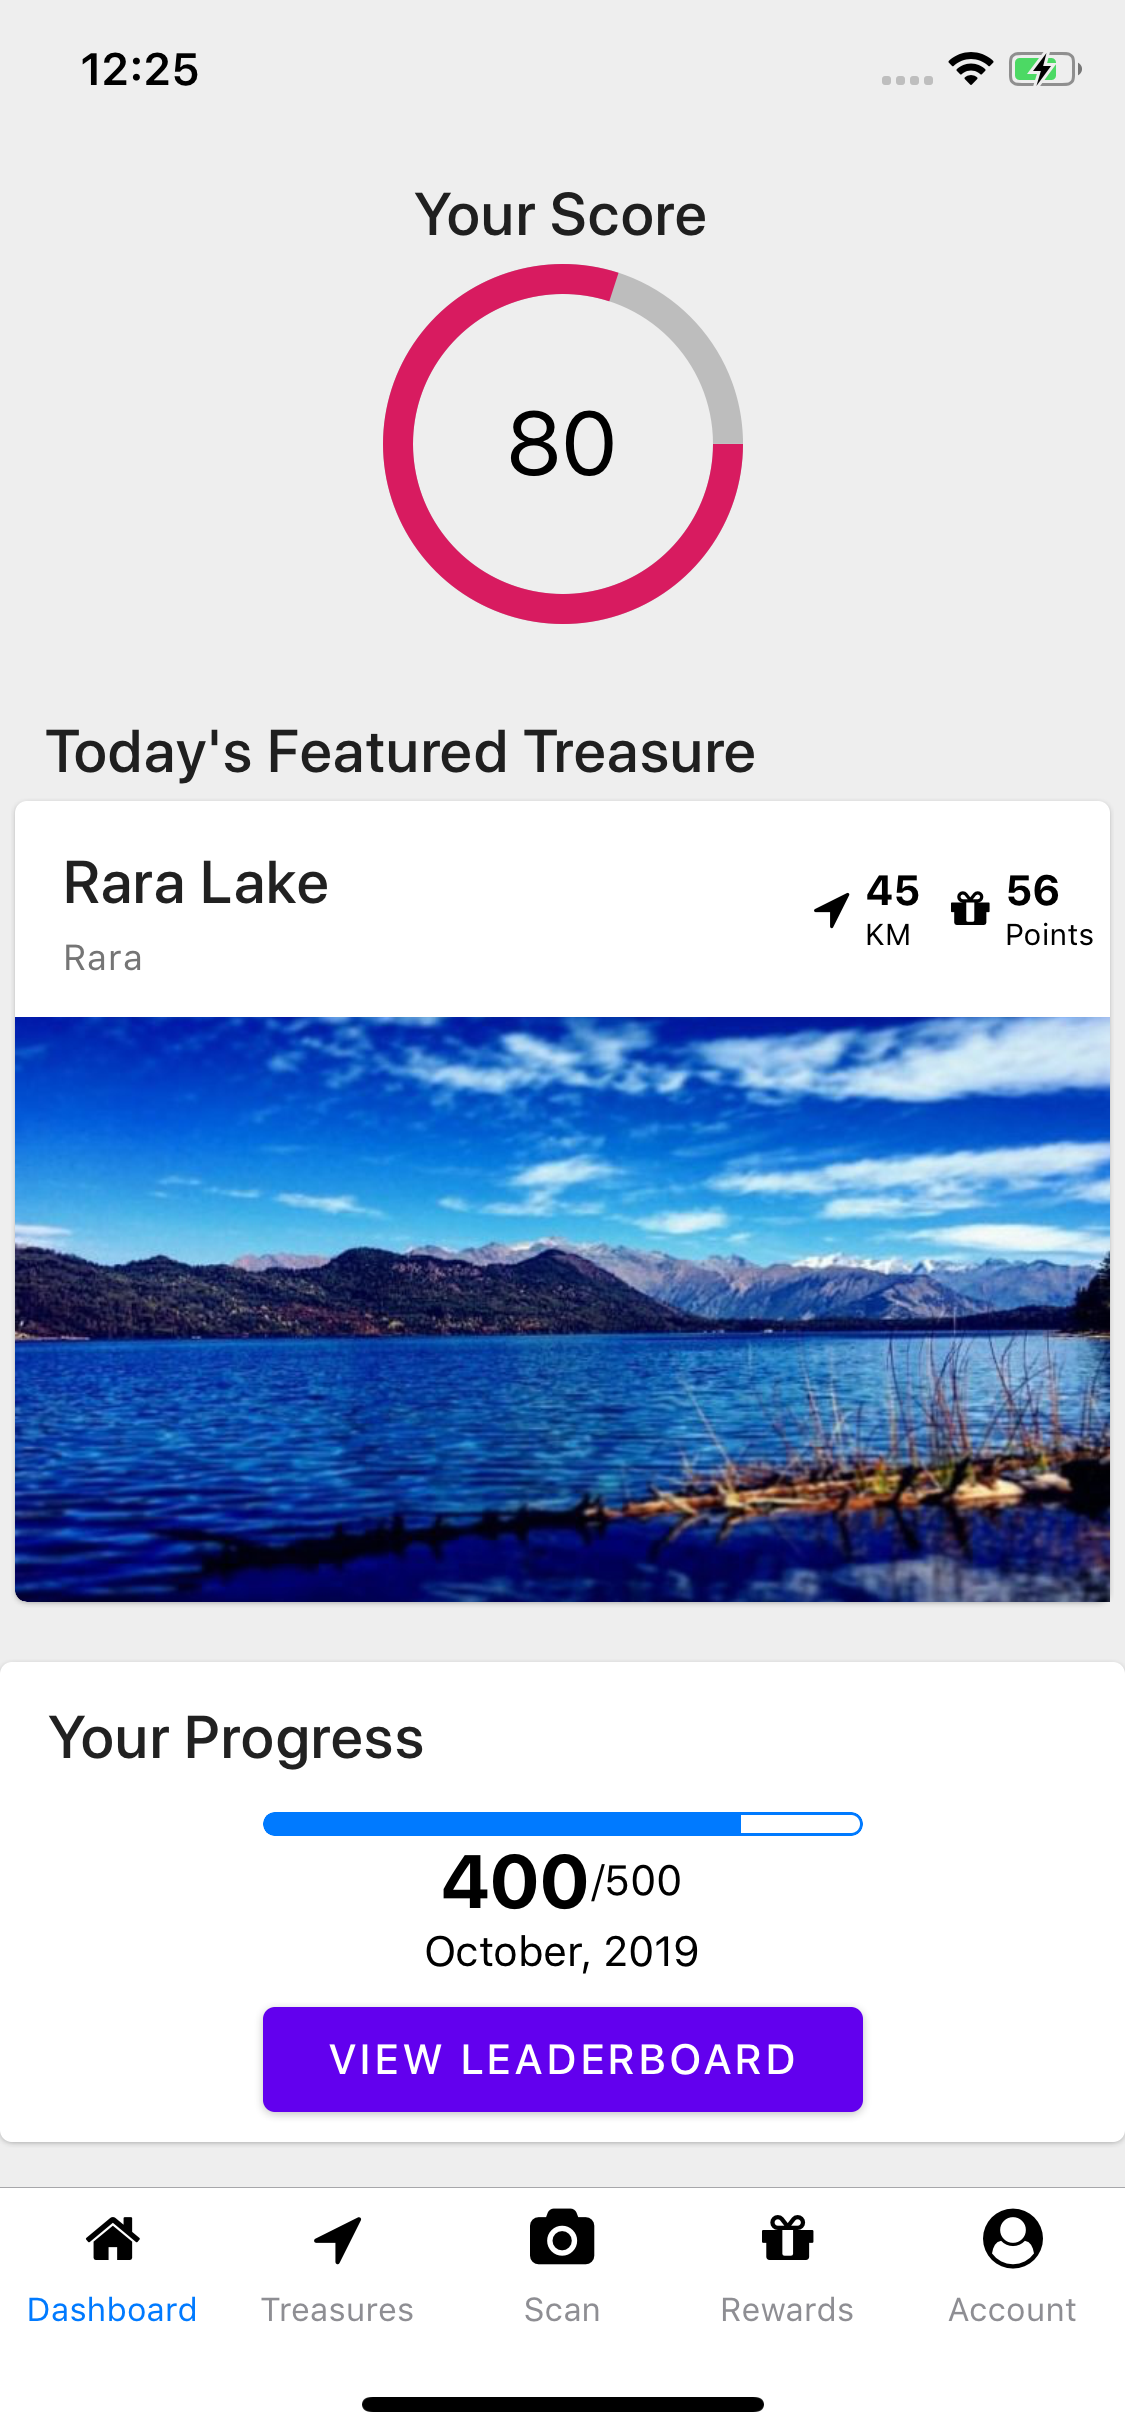
\includegraphics[width=0.45\textwidth]{test-evidences/auth/b.png}
    \caption{}
\end{subfigure}

\begin{subfigure}{.5\textwidth}
    \centering
    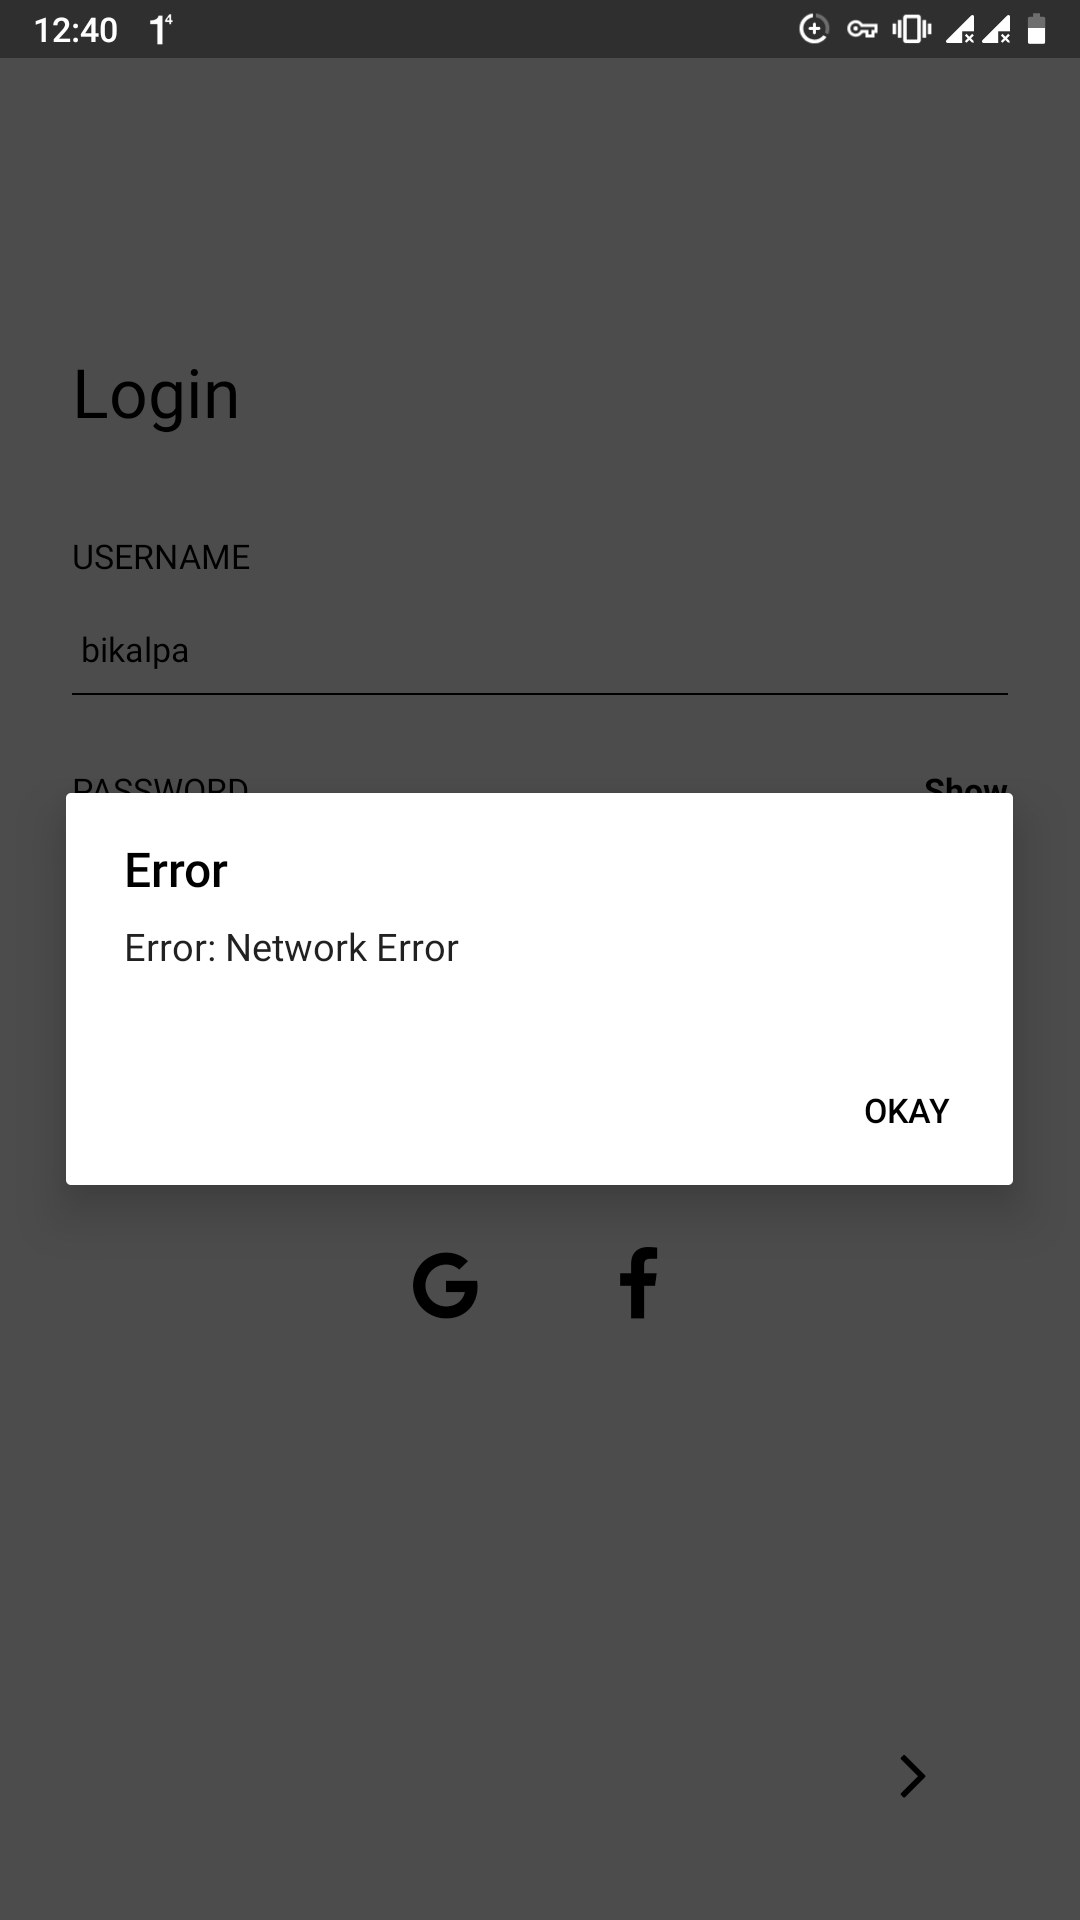
\includegraphics[width=0.45\textwidth]{test-evidences/auth/c.png}
    \caption{}
\end{subfigure}%
\begin{subfigure}{.5\textwidth}
    \centering
    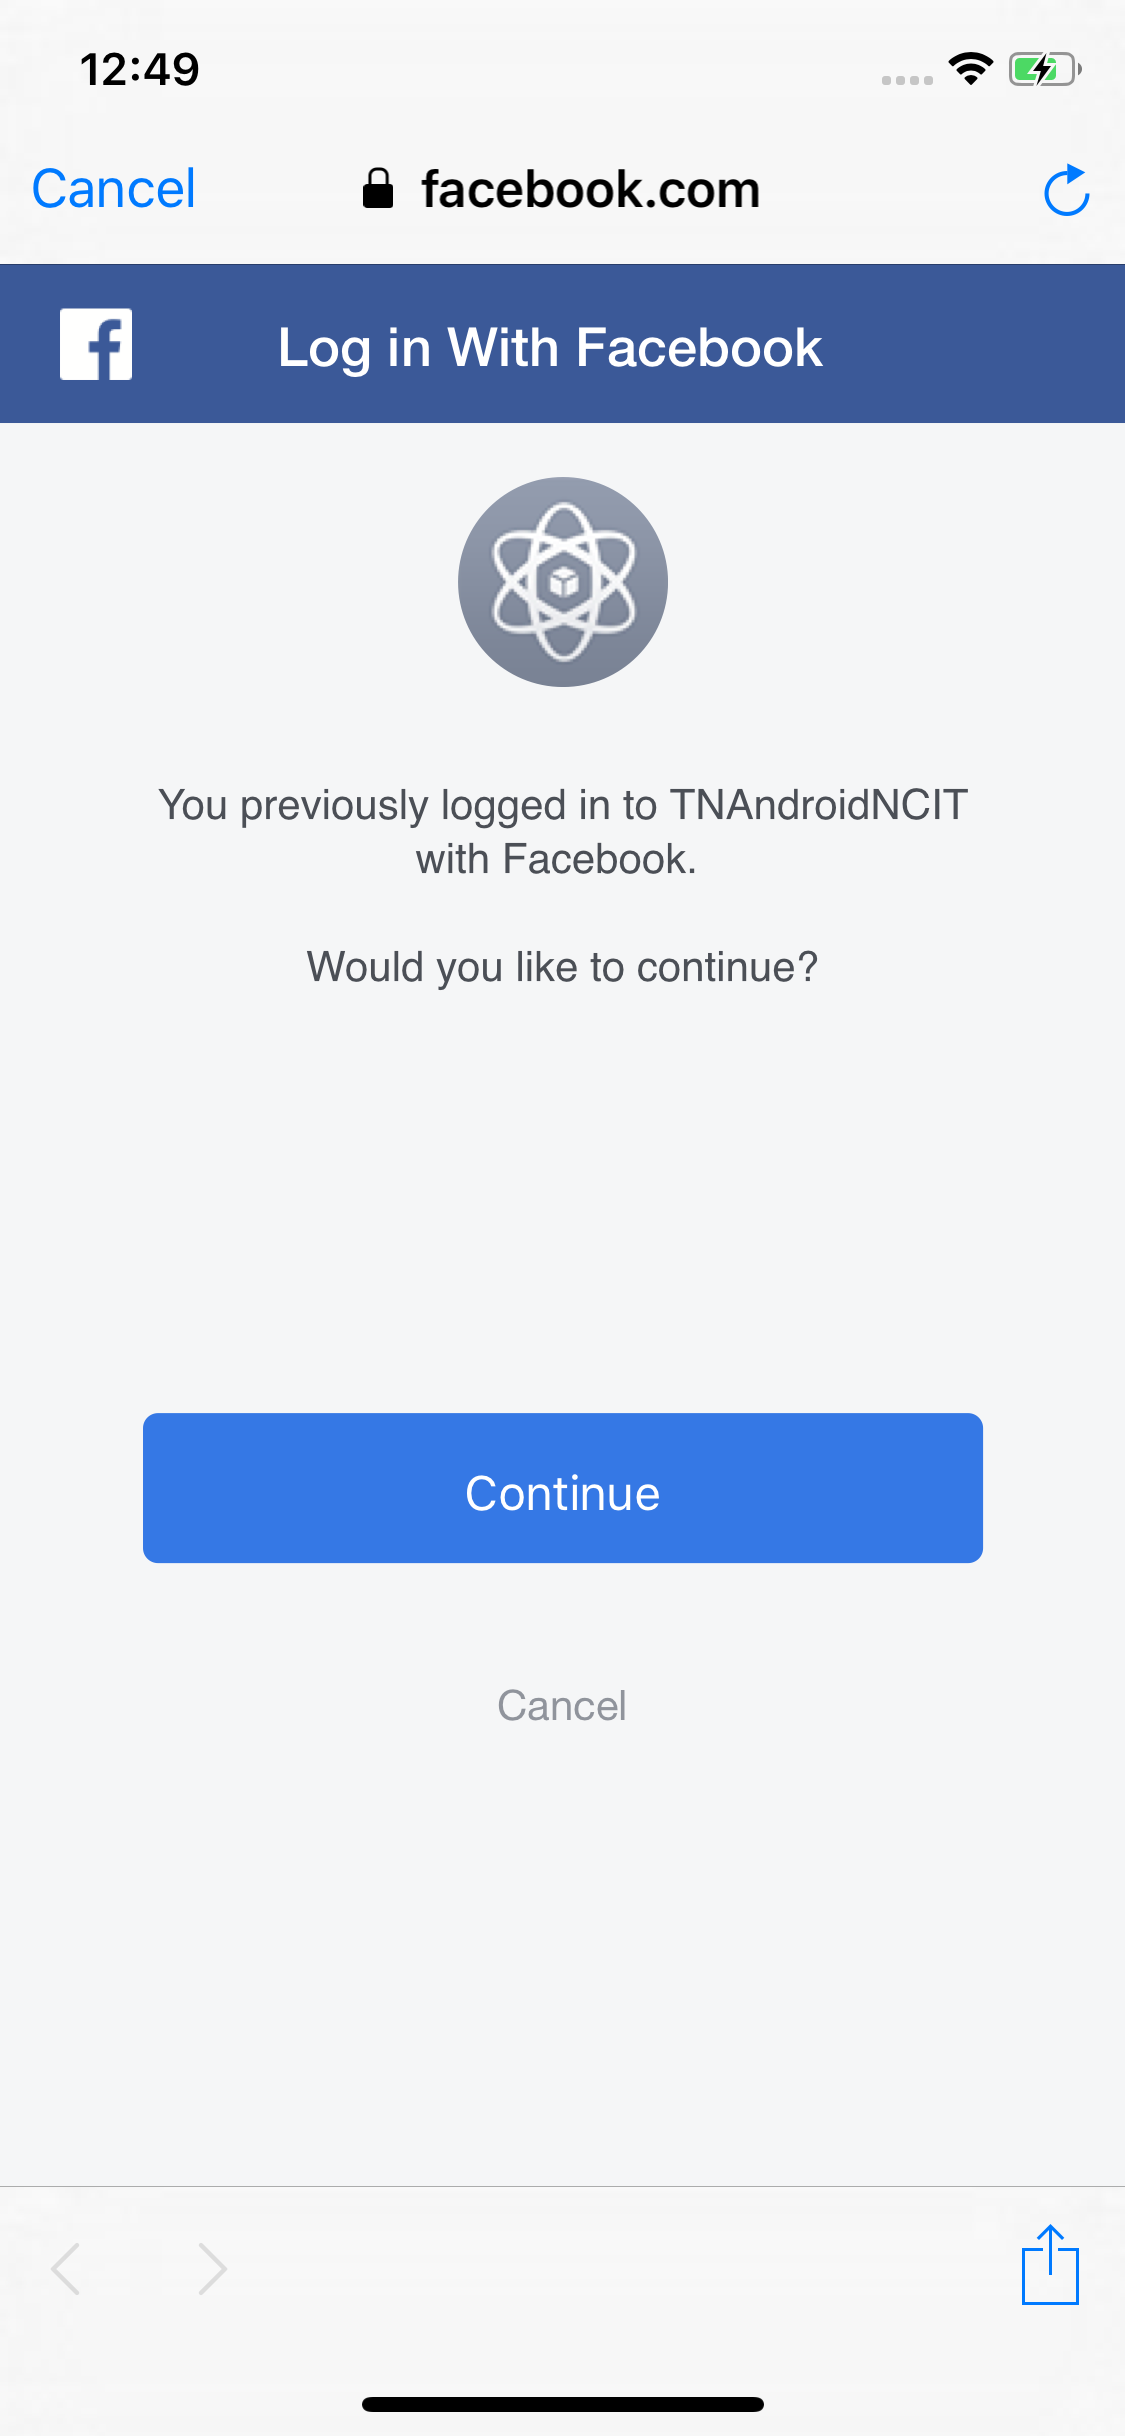
\includegraphics[width=0.45\textwidth]{test-evidences/auth/d.png}
    \caption{}
\end{subfigure}

\begin{subfigure}{.5\textwidth}
    \centering
    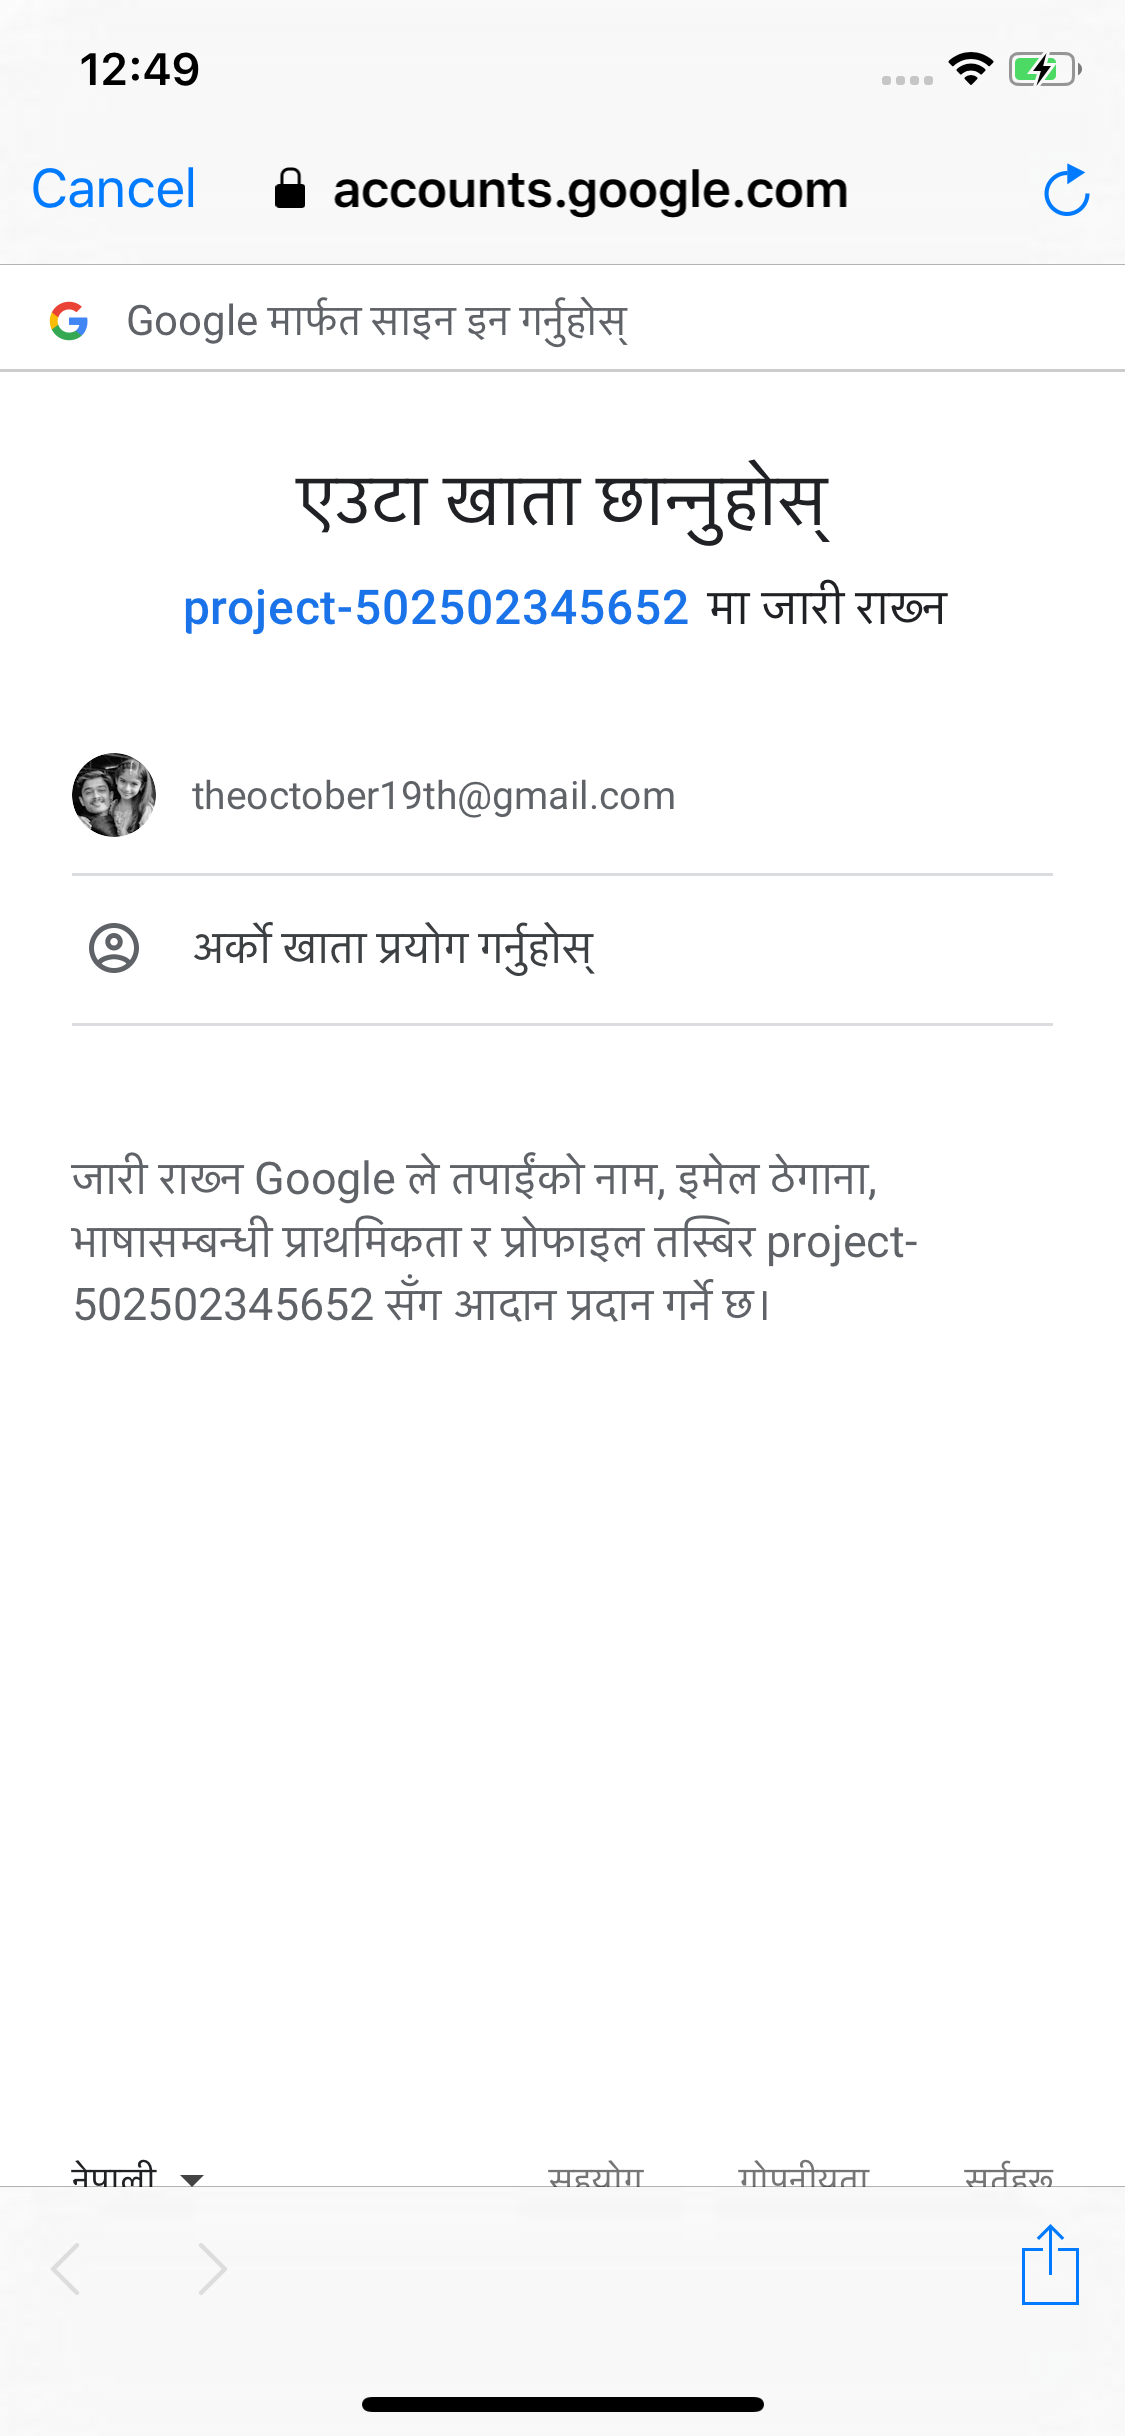
\includegraphics[width=0.45\textwidth]{test-evidences/auth/e.png}
    \caption{}
\end{subfigure}%
\begin{subfigure}{.5\textwidth}
    \centering
    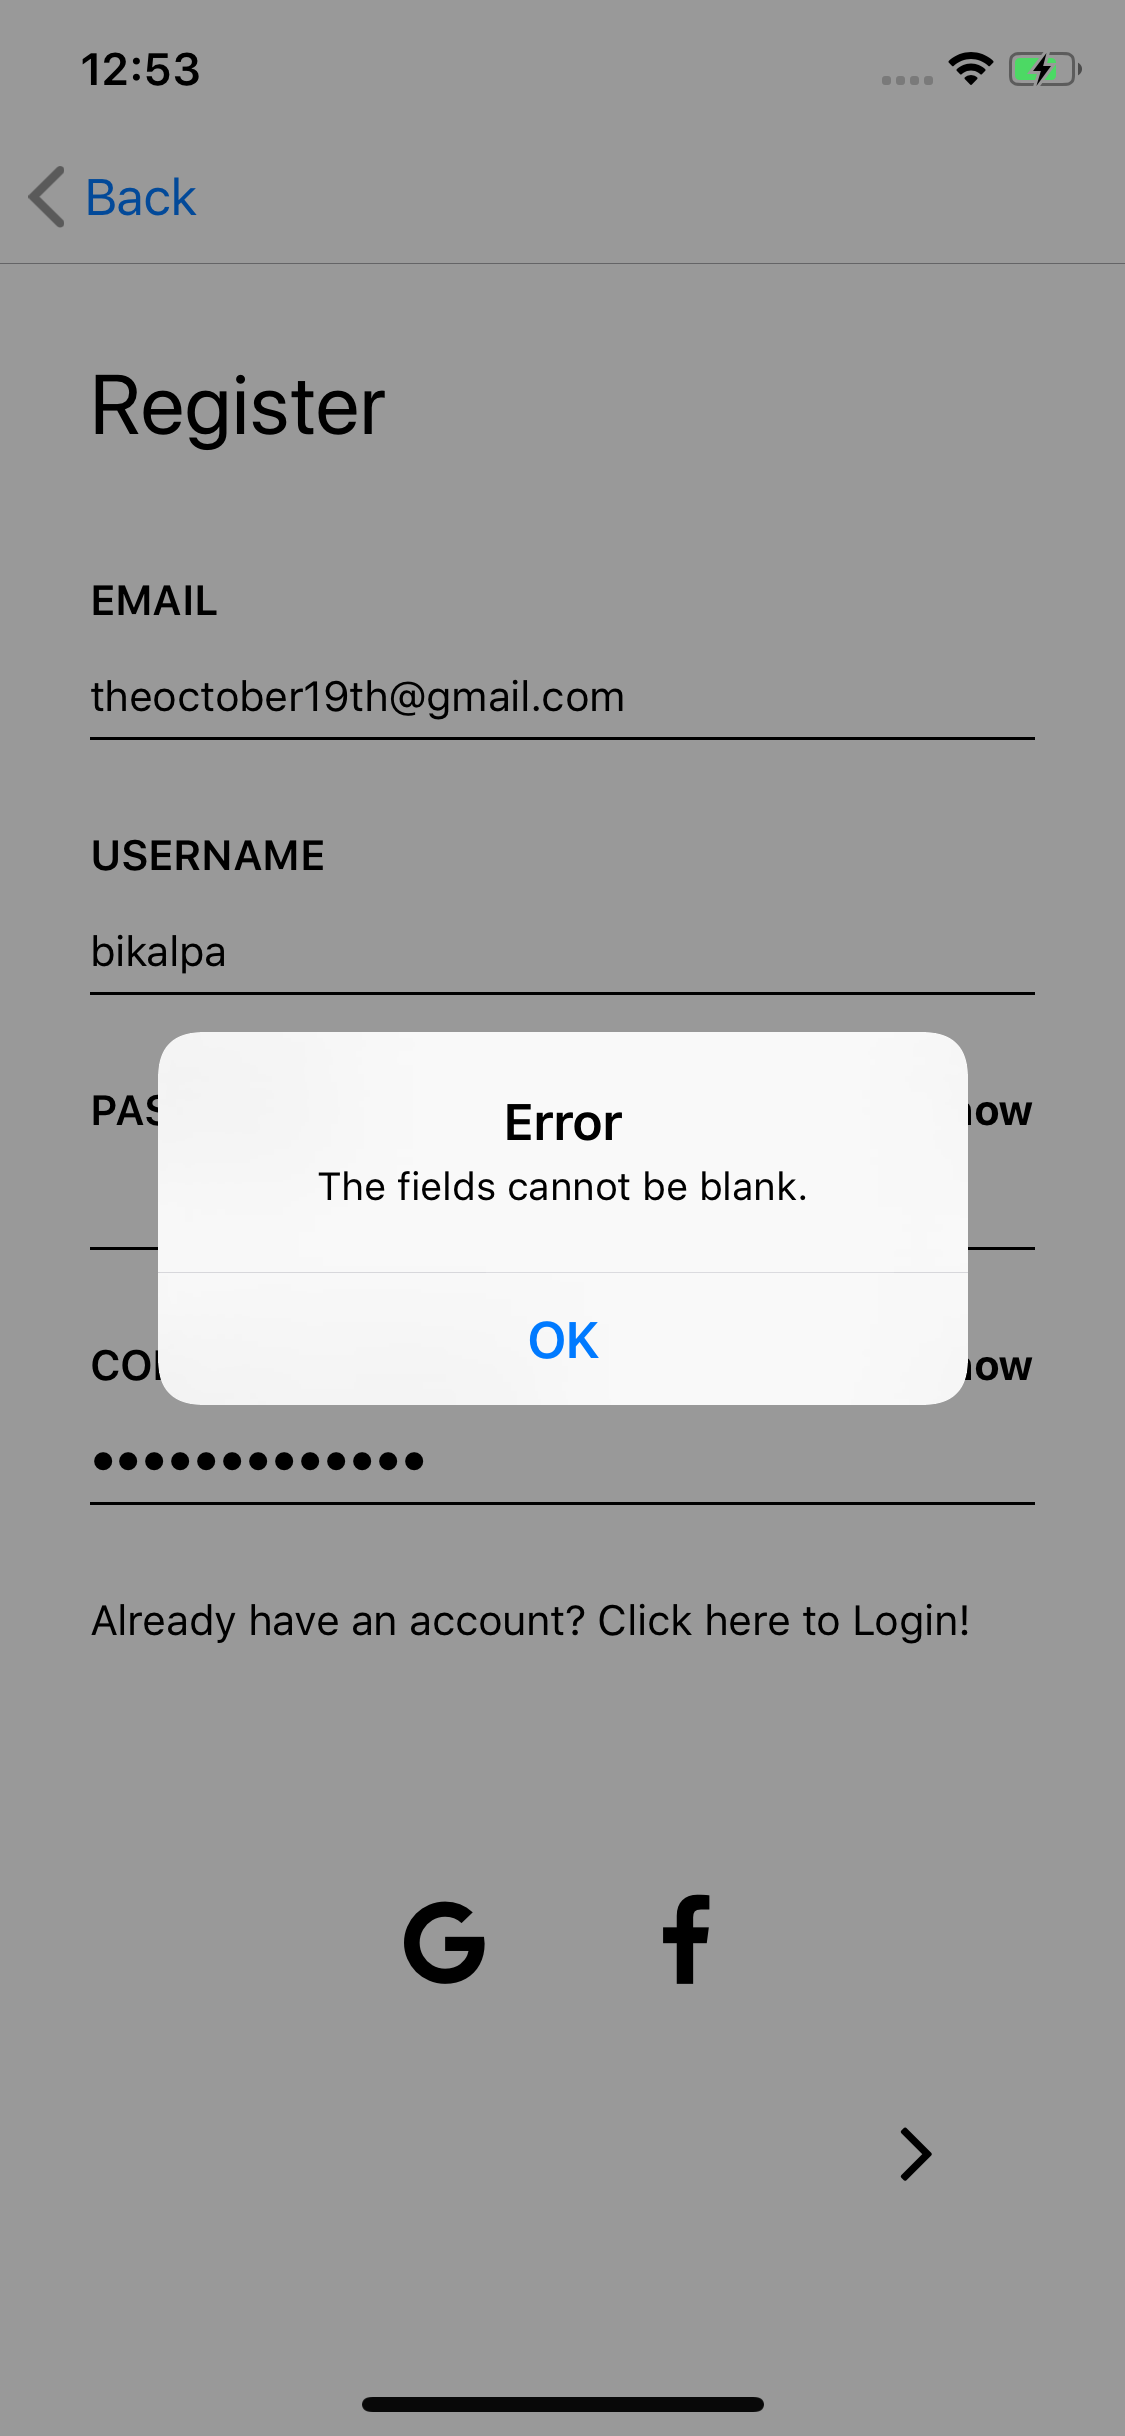
\includegraphics[width=0.45\textwidth]{test-evidences/auth/f.png}
    \caption{}
\end{subfigure}


\caption{Test success evidences for unit authentication}
\label{fig:test-evidence-auth}
\end{figure}


\begin{figure}[H]

\begin{subfigure}{.5\textwidth}
    \centering
    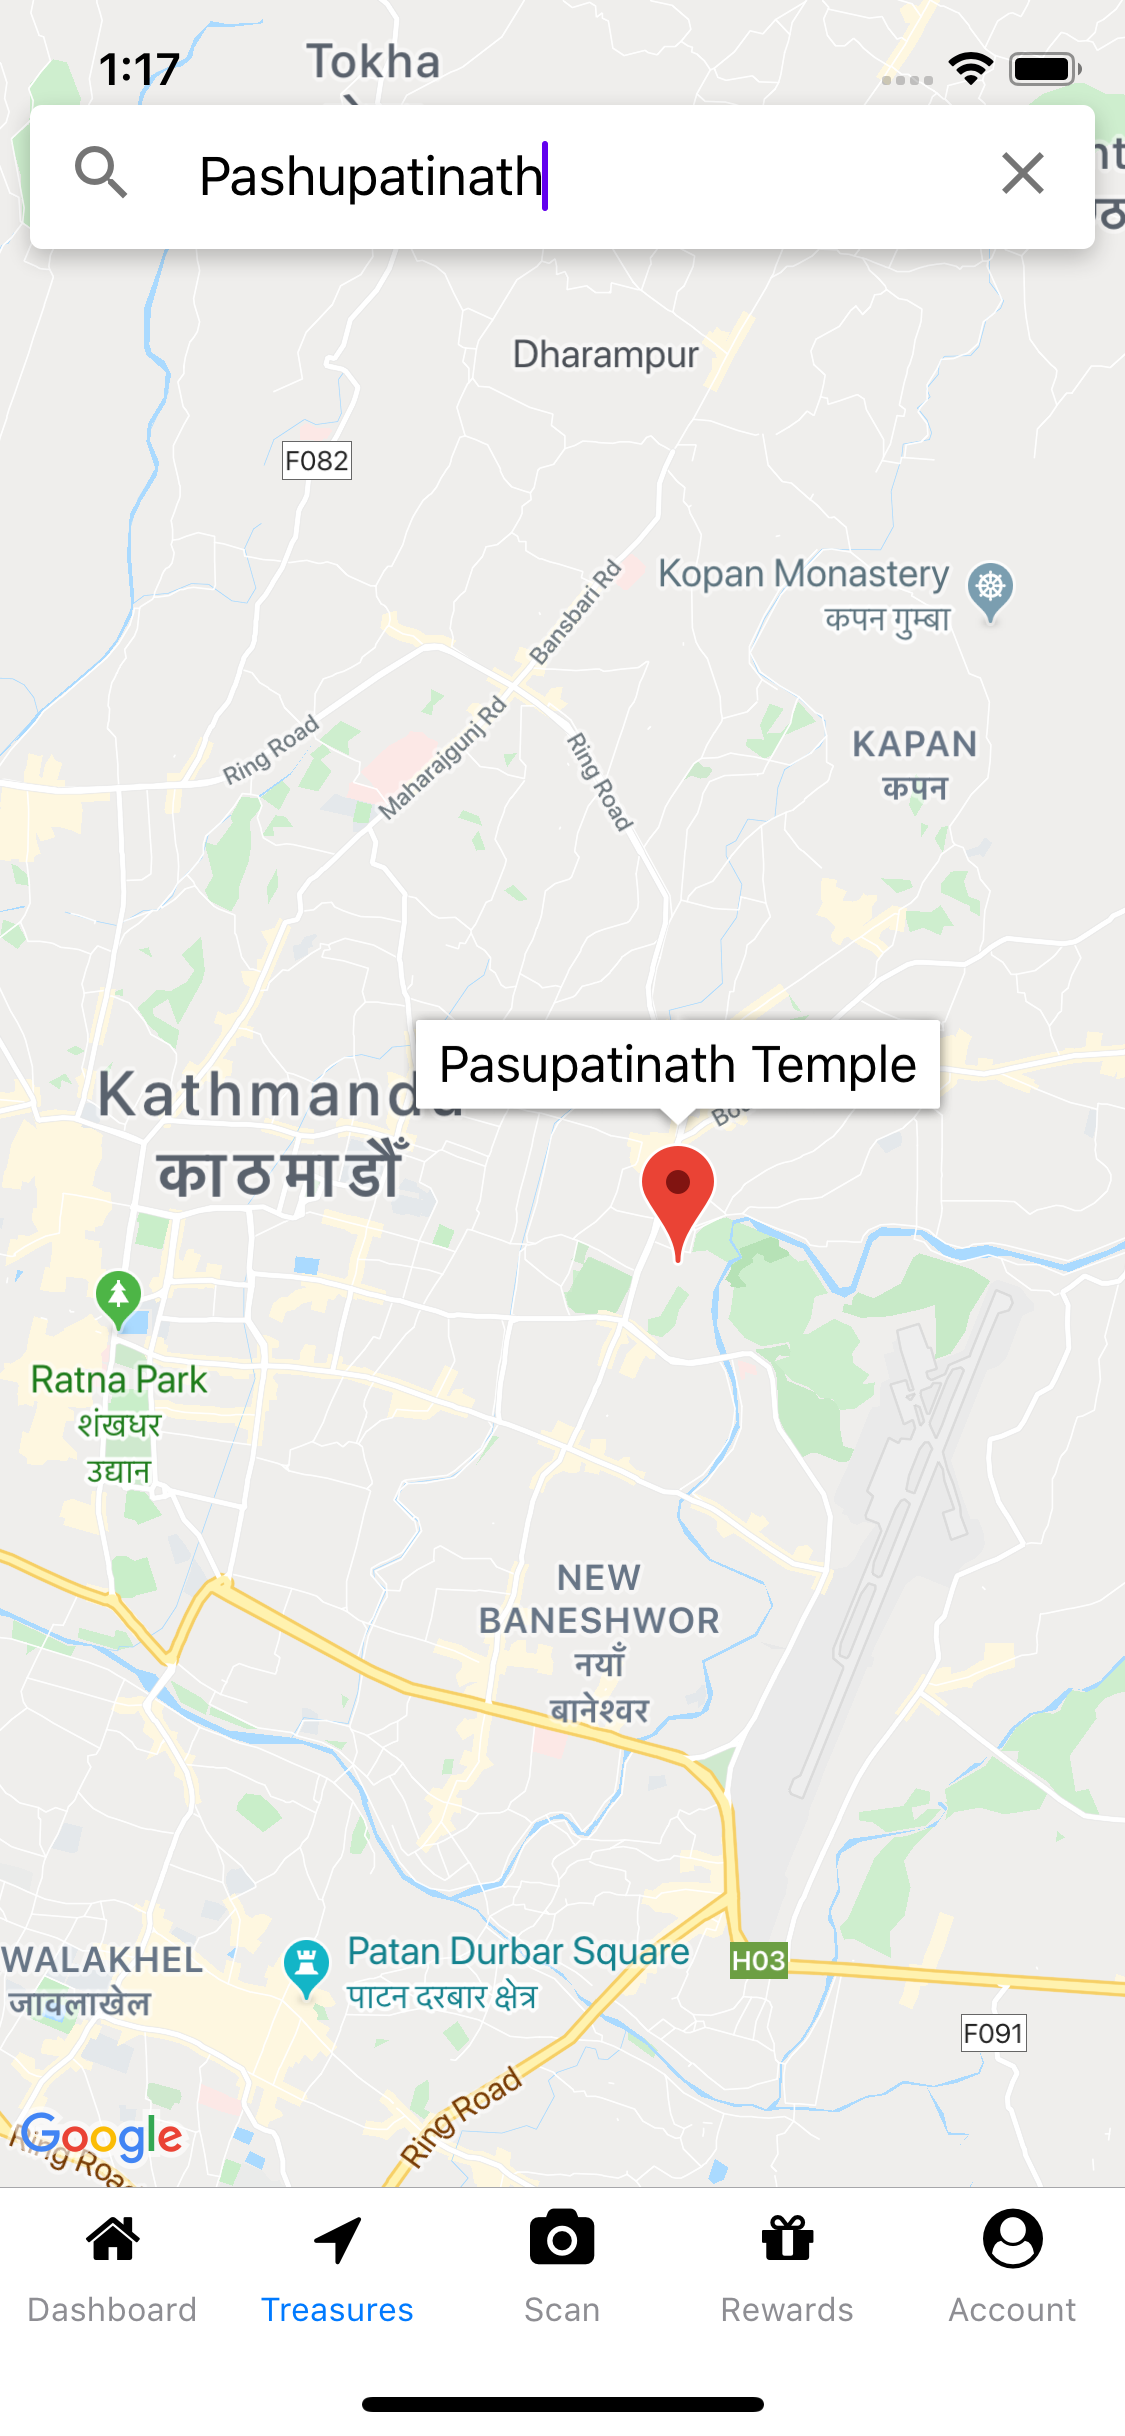
\includegraphics[width=0.45\textwidth]{test-evidences/treasure/a.png}
    \caption{}
\end{subfigure}%
\begin{subfigure}{.5\textwidth}
    \centering
    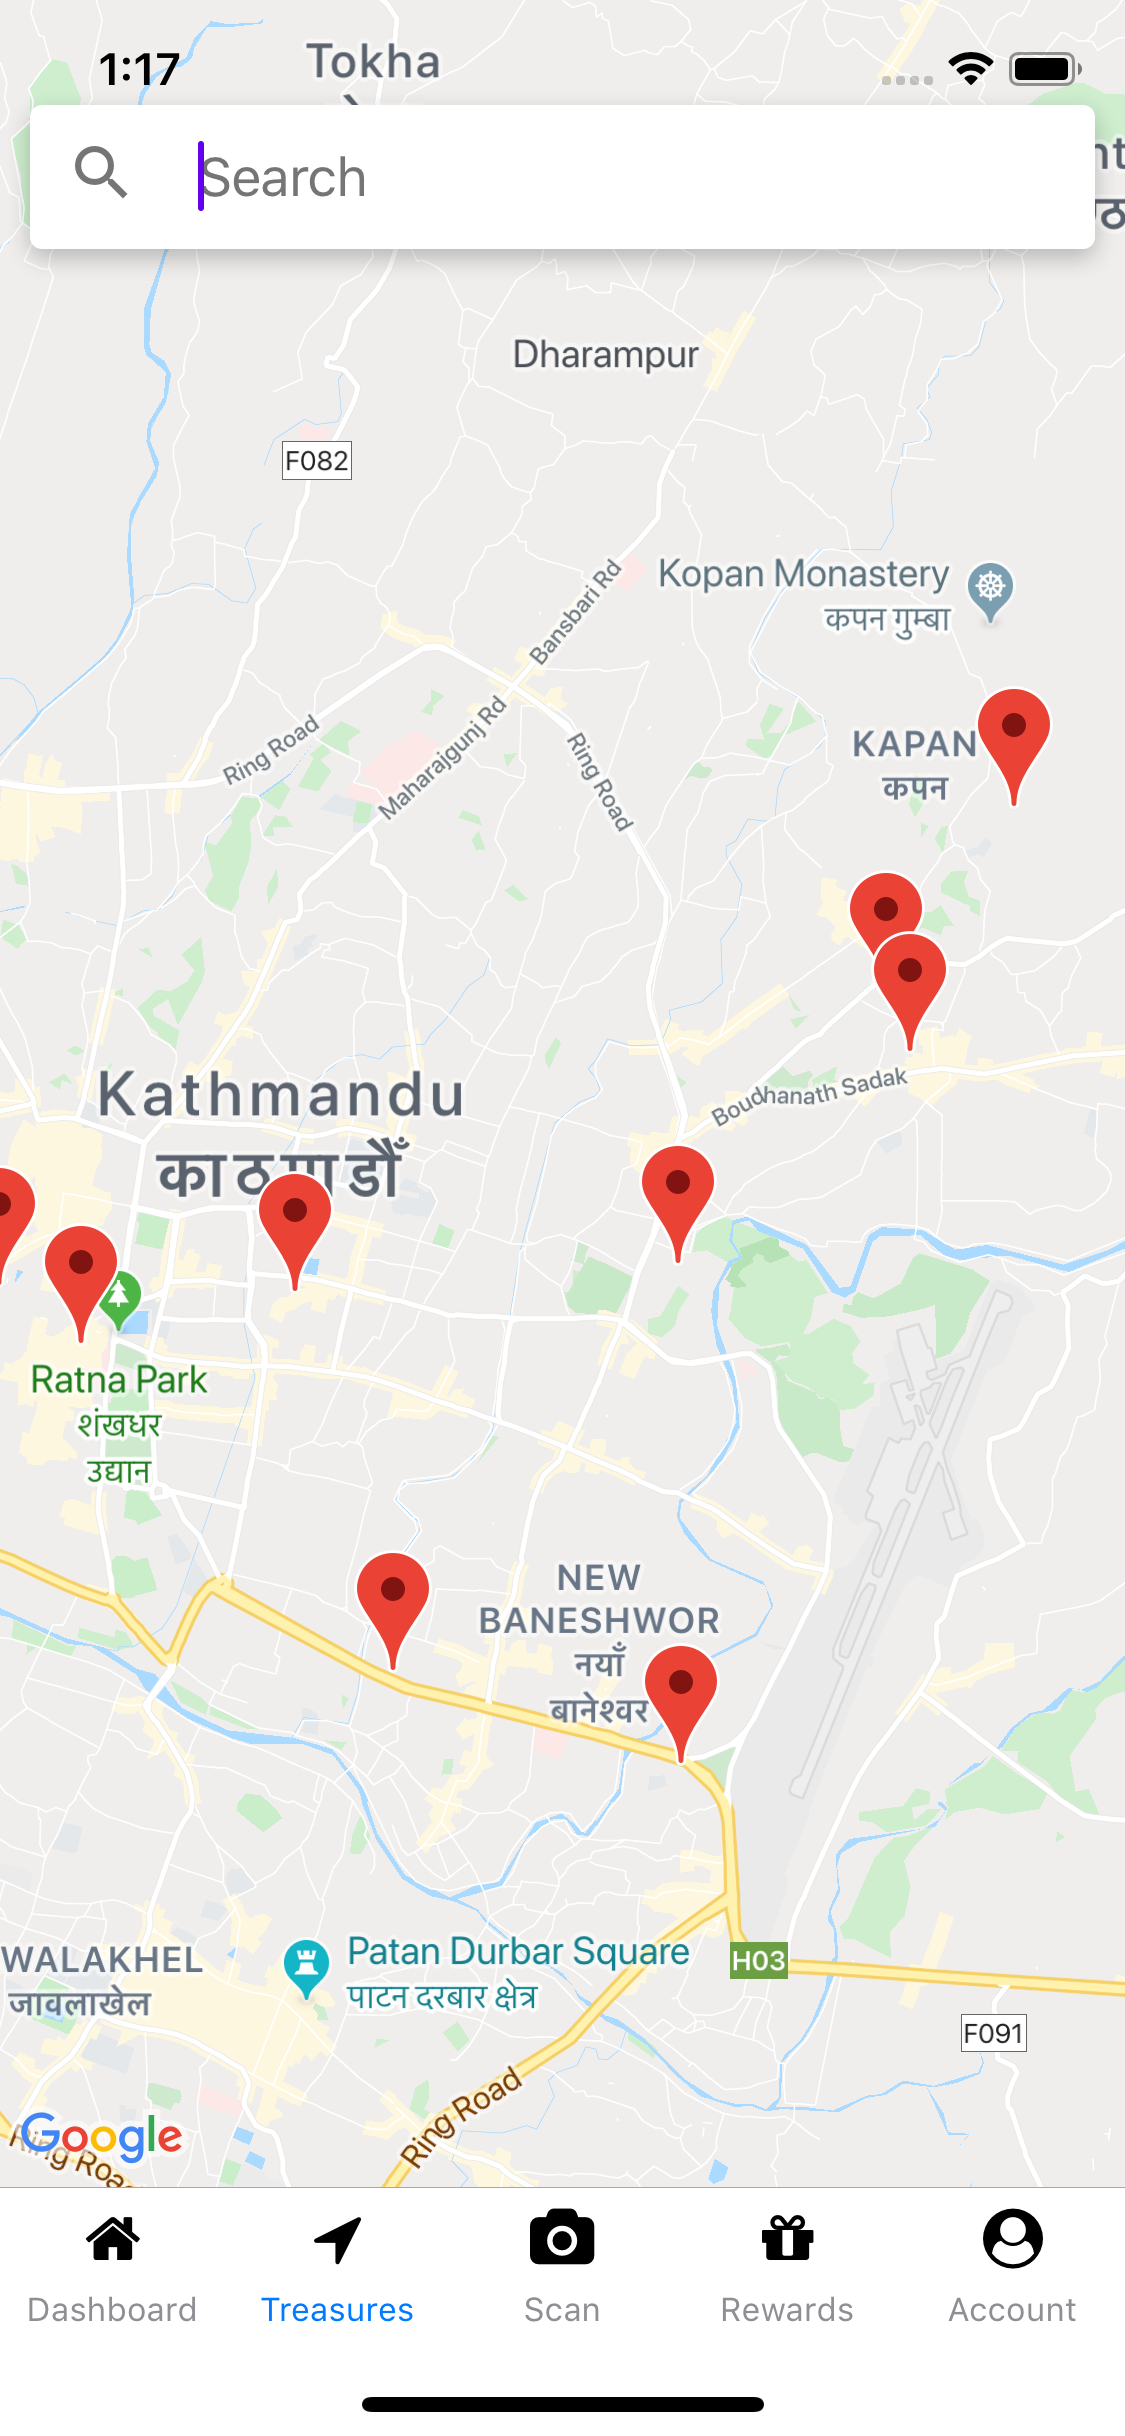
\includegraphics[width=0.45\textwidth]{test-evidences/treasure/b.png}
    \caption{}
\end{subfigure}

\begin{subfigure}{.5\textwidth}
    \centering
    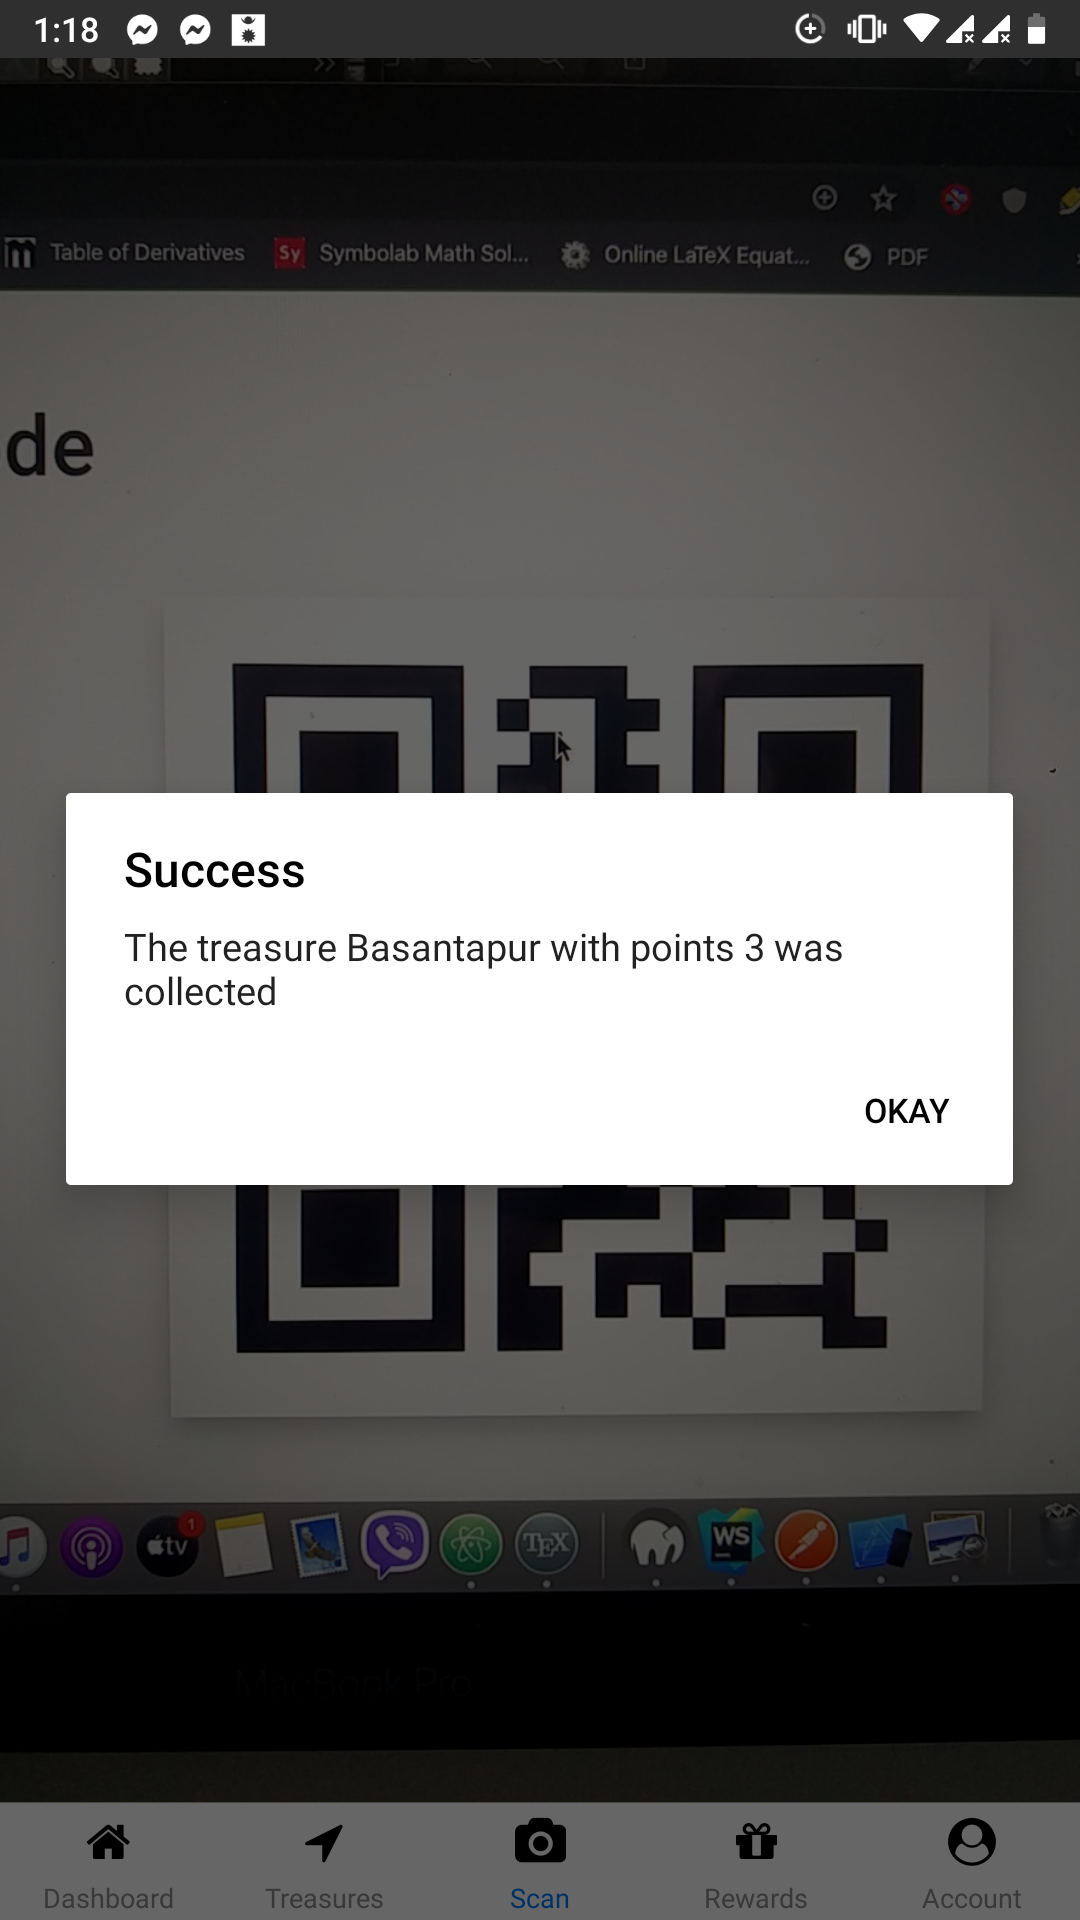
\includegraphics[width=0.45\textwidth]{test-evidences/treasure/c.png}
    \caption{}
\end{subfigure}%
\begin{subfigure}{.5\textwidth}
    \centering
    \includegraphics[width=0.45\textwidth]{test-evidences/treasure/d.png}
    \caption{}
\end{subfigure}

\begin{subfigure}{.5\textwidth}
    \centering
    \includegraphics[width=0.45\textwidth]{test-evidences/treasure/e.png}
    \caption{}
\end{subfigure}%
\begin{subfigure}{.5\textwidth}
    \centering
    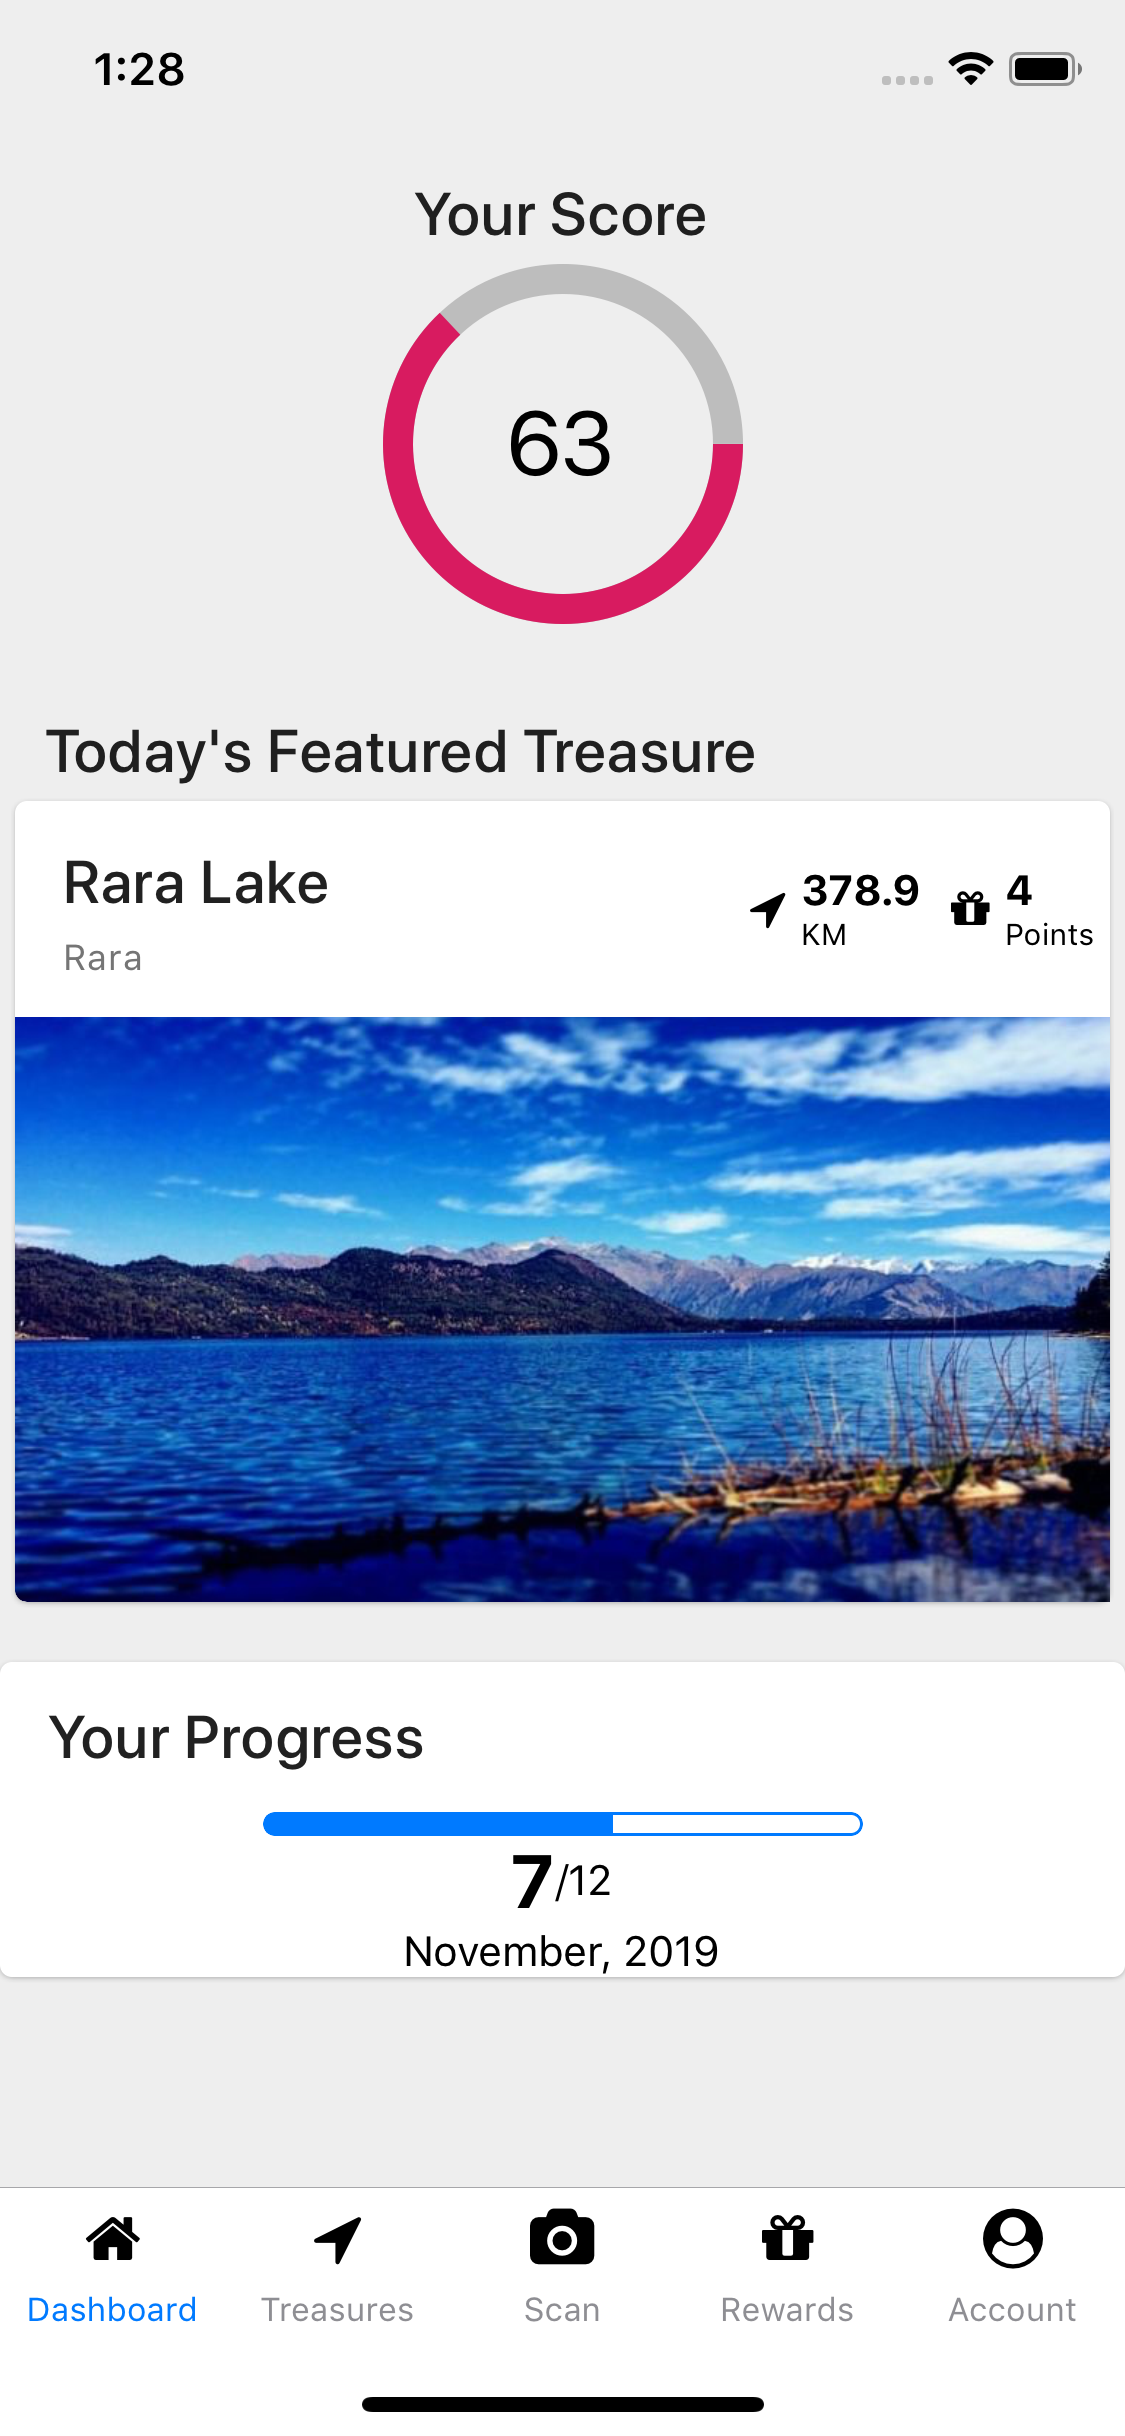
\includegraphics[width=0.45\textwidth]{test-evidences/treasure/f.png}
    \caption{}
\end{subfigure}


\caption{Test success evidences for treasure unit test}
\label{fig:test-evidence-treasure}
\end{figure}

\begin{figure}[H]

\begin{subfigure}{.5\textwidth}
    \centering
    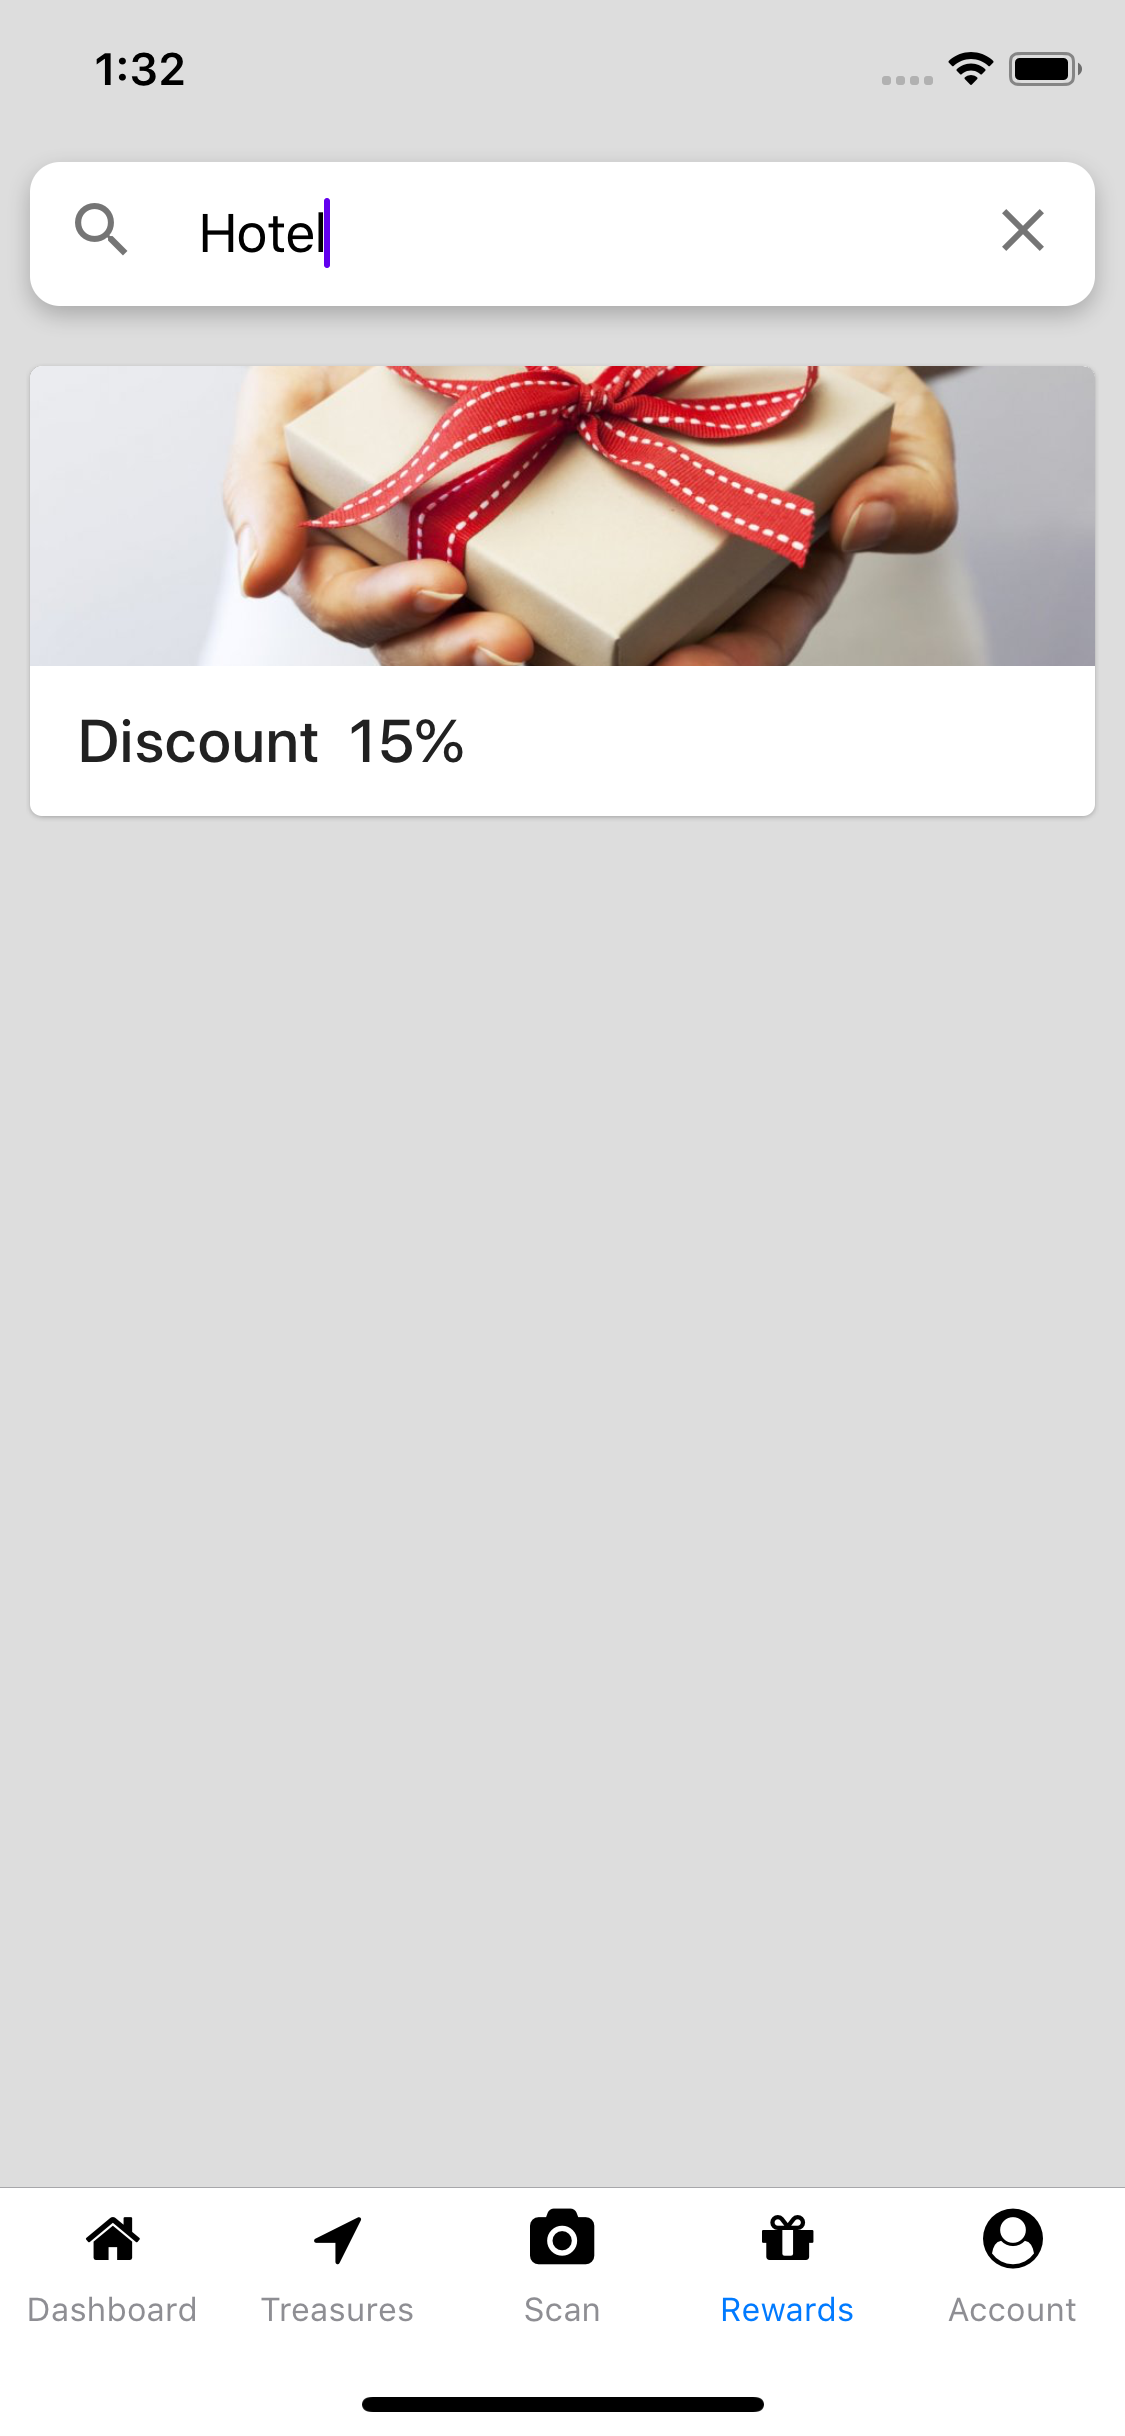
\includegraphics[width=0.45\textwidth]{test-evidences/reward/a.png}
    \caption{}
\end{subfigure}%
\begin{subfigure}{.5\textwidth}
    \centering
    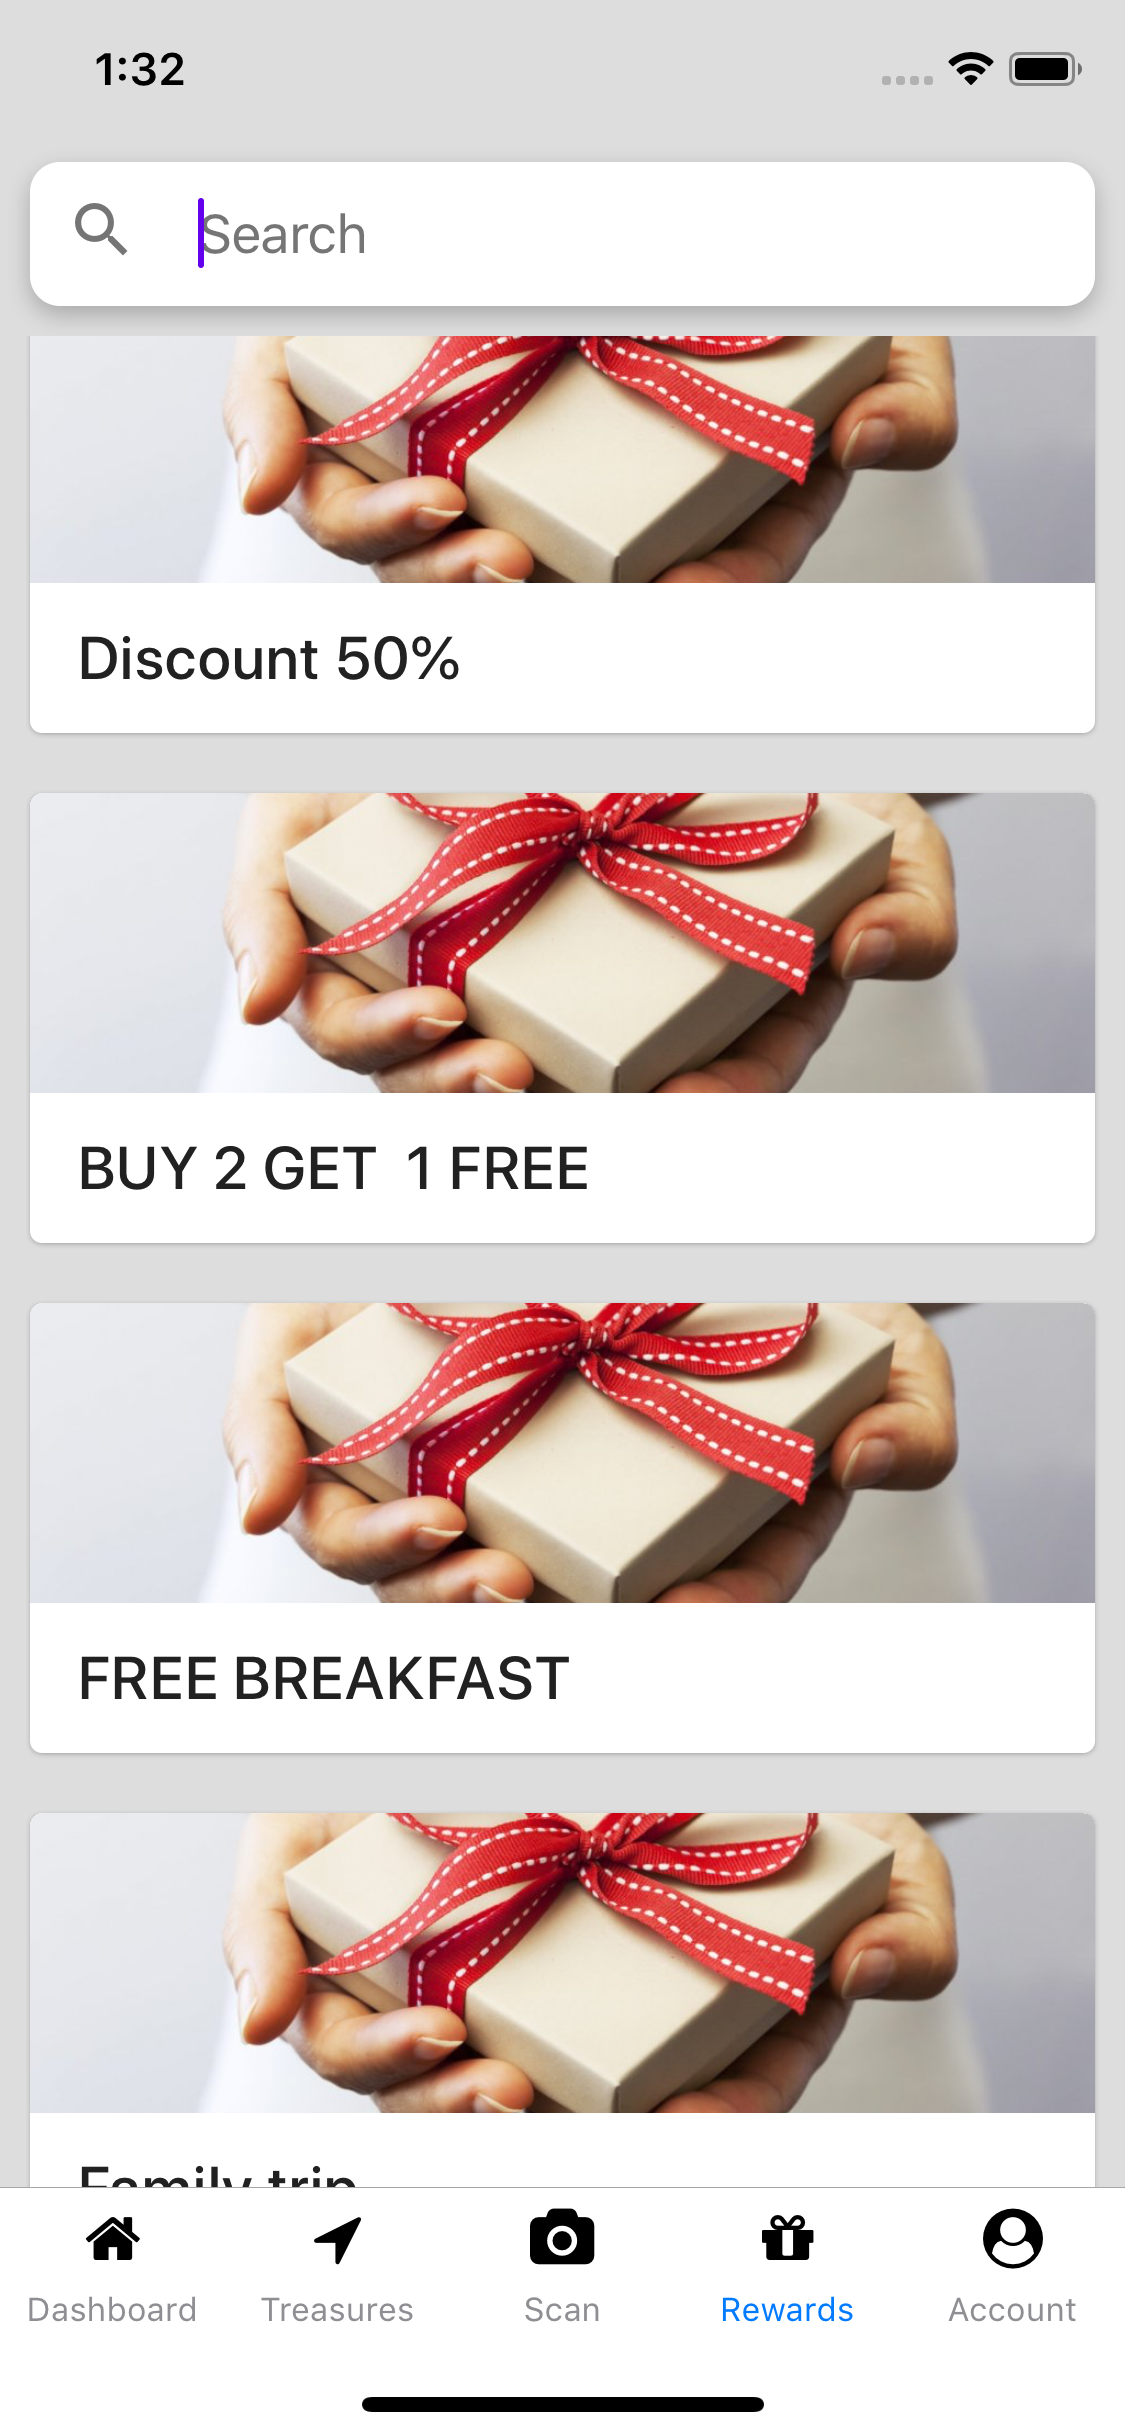
\includegraphics[width=0.45\textwidth]{test-evidences/reward/b.png}
    \caption{}
\end{subfigure}

\begin{subfigure}{.5\textwidth}
    \centering
    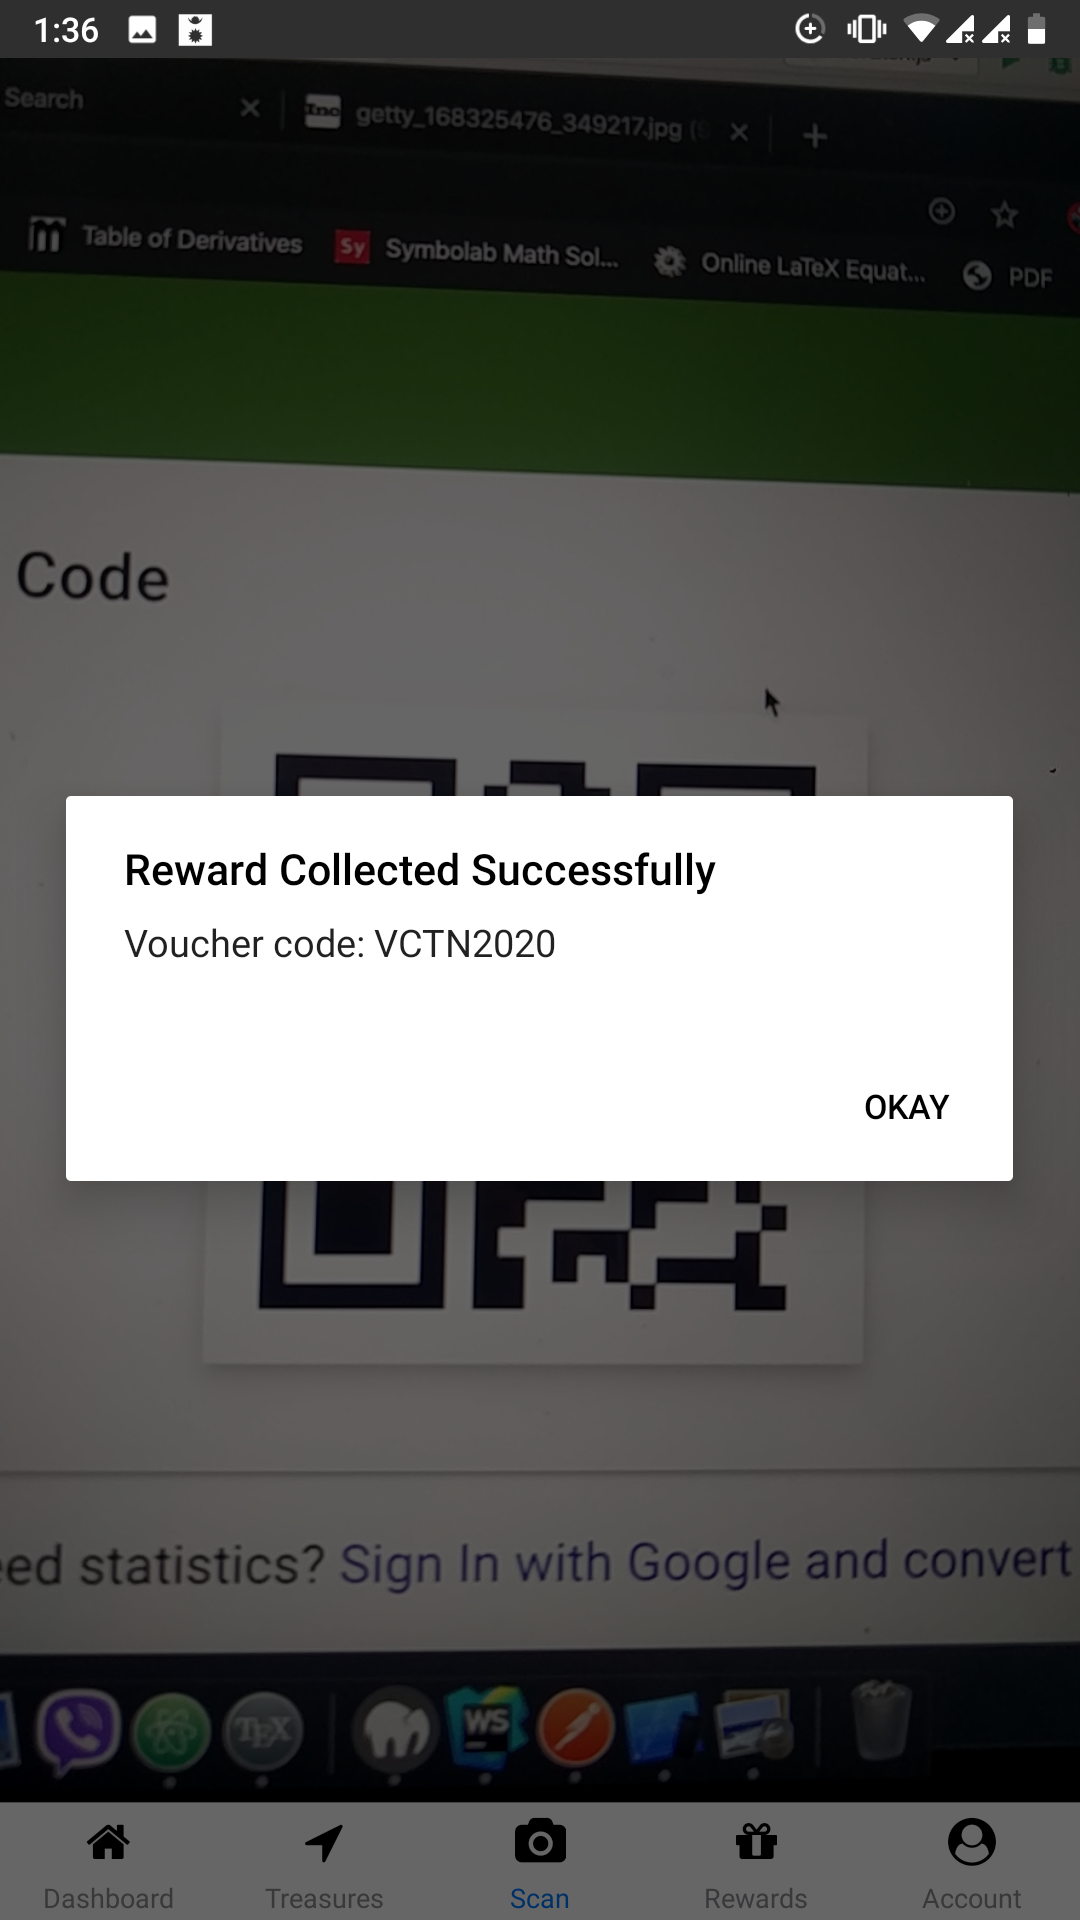
\includegraphics[width=0.45\textwidth]{test-evidences/reward/c.png}
    \caption{}
\end{subfigure}%
\begin{subfigure}{.5\textwidth}
    \centering
    \includegraphics[width=0.45\textwidth]{test-evidences/reward/d.png}
    \caption{}
\end{subfigure}

\begin{subfigure}{.5\textwidth}
    \centering
    \includegraphics[width=0.45\textwidth]{test-evidences/reward/e.png}
    \caption{}
\end{subfigure}%
\begin{subfigure}{.5\textwidth}
    \centering
    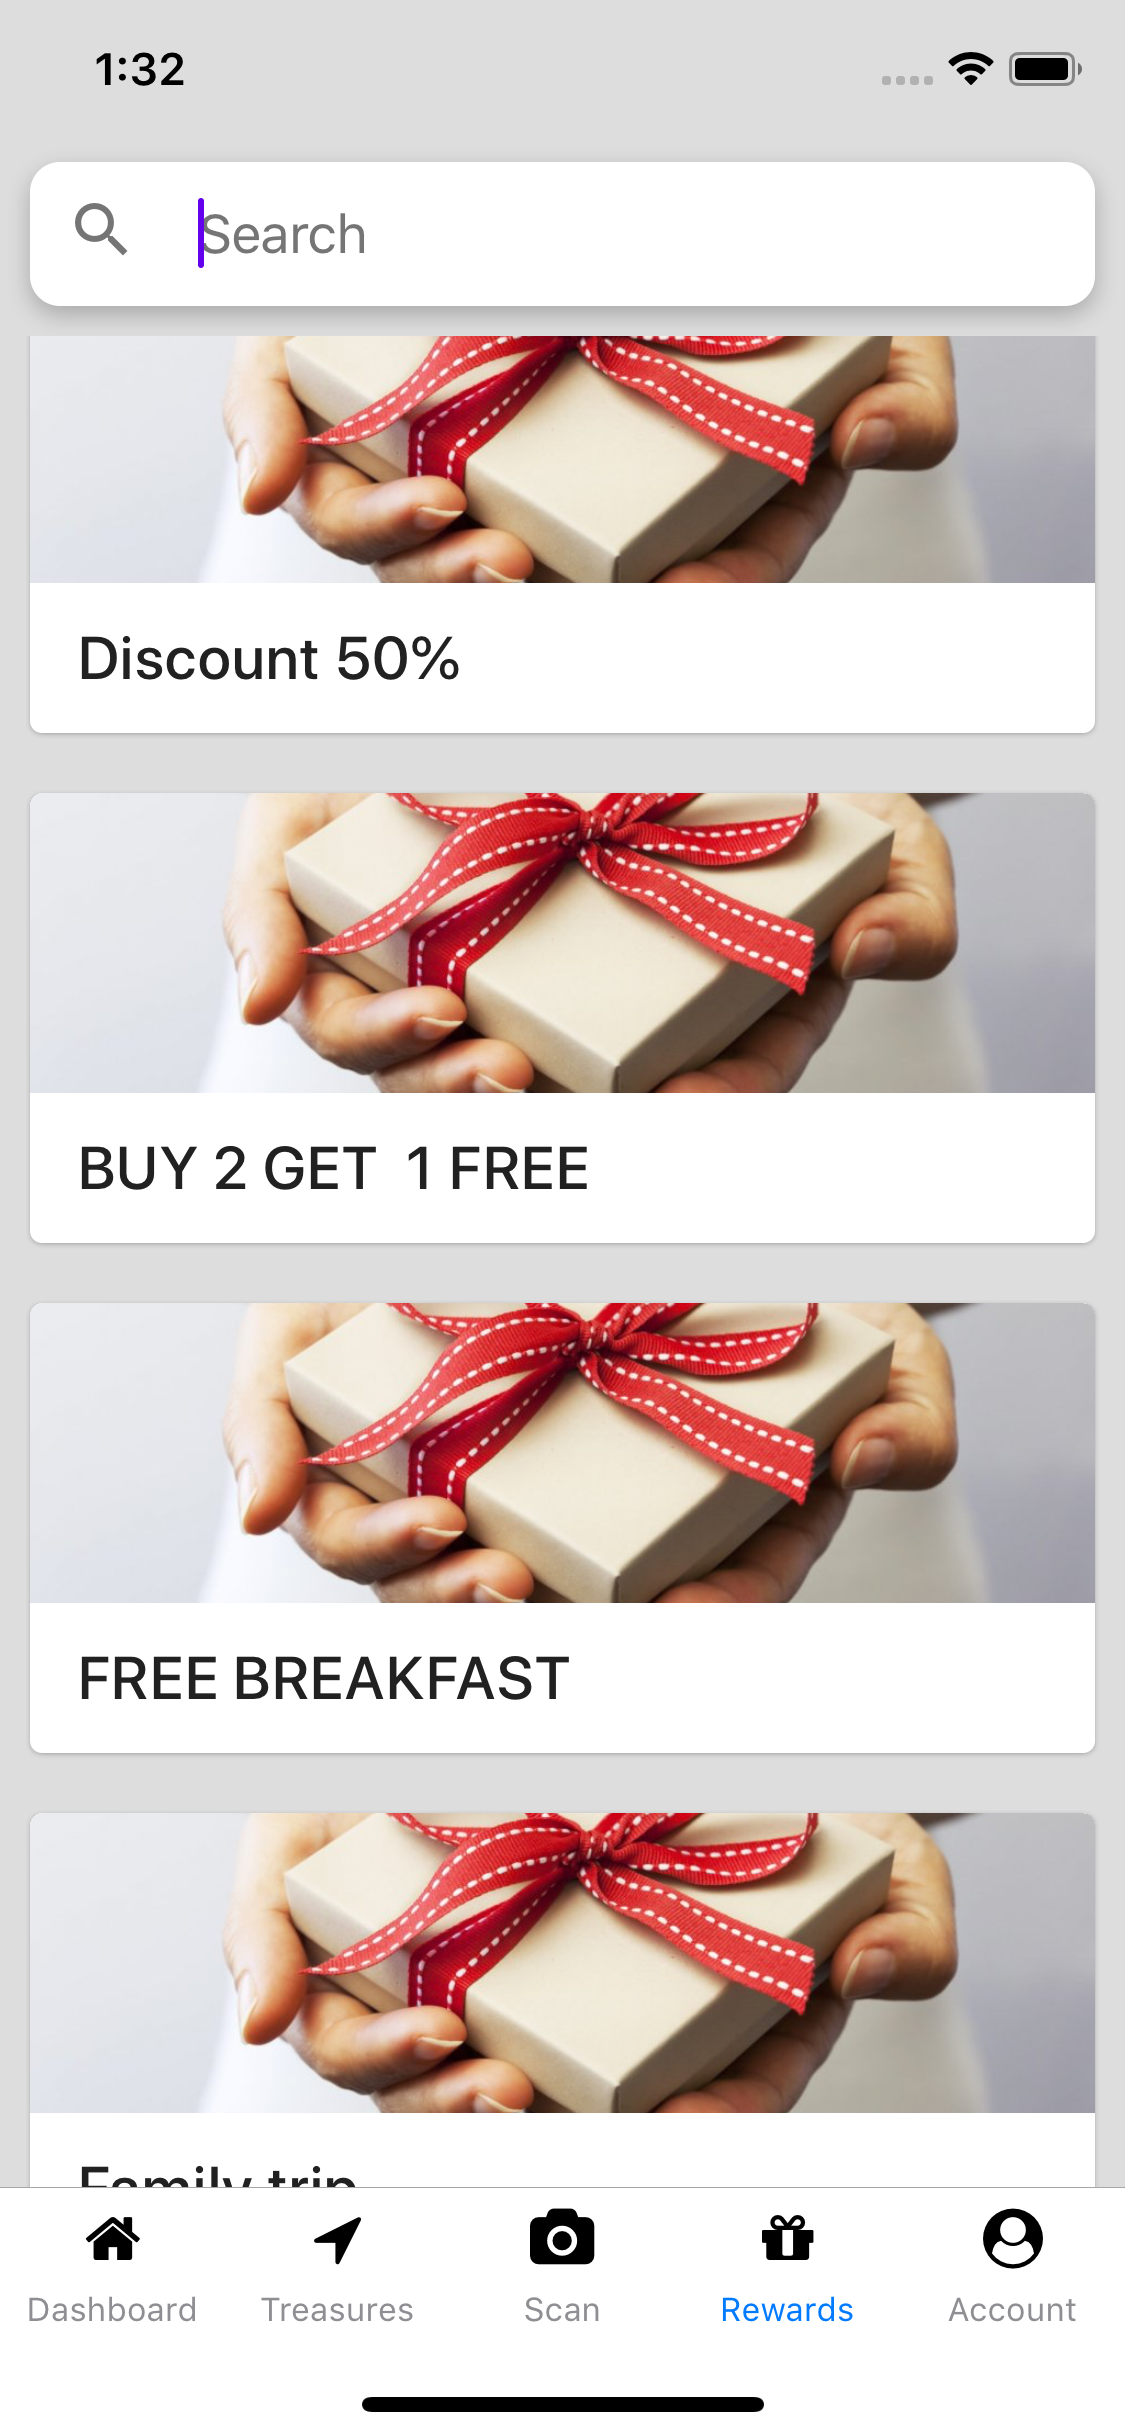
\includegraphics[width=0.45\textwidth]{test-evidences/reward/f.png}
    \caption{}
\end{subfigure}


\caption{Test success evidences for reward unit test}
\label{fig:test-evidence-reward}
\end{figure}

\subsection{Debugging}
This section consists of various changes applied during debugging process to those test cases that didn't pass in the section \ref{testcases}. The test cases that didn't pass were inspected for the root cause of the problem, the problems were identified, resolved and the test case was applied again to see if it succeeds.

\begin{table}[H]
\begin{tabularx}{\linewidth}{|c|X|}
\hline
\rowcolor[HTML]{C0C0C0} 
ID                 & DL01                                                                       \\ \hline
Test Case          & TL03                                                                       \\ \hline
Scenario           & Enter valid login credentials, turn off network connection and then log in \\ \hline
Data               & username: valid  password: valid                                           \\ \hline
Expected Outcome   & User gets 'Network Connection Error'                                       \\ \hline
Actual Outcome     & Progress spinner spins infinitely                                          \\ \hline
Reason for Failure & Exception for network error was missing                                    \\ \hline
Changes made       & Exception clause for the NetworkException was added                        \\ \hline                  
\end{tabularx}
\caption{Debugging error of test case TL03}
\end{table}

\begin{table}[H]
\begin{tabularx}{\linewidth}{|c|X|}
\hline
\rowcolor[HTML]{C0C0C0} 
ID                 & DL02                                                                       \\ \hline
Test Case          & TL06                                                                       \\ \hline
Scenario           & After being logged in, user closes the app, clears all running apps and opens app again \\ \hline
Expected Outcome   & User should directly see the Dashboard page                                       \\ \hline
Actual Outcome     & User is navigated back to Login Page                                          \\ \hline
Reason for Failure & Authentication status of user was written in memory, but not in persistent storage of device. As a result, the value got destroyed when he app was cleared from memory.                                    \\ \hline
Changes made       & The flag storing the authentication status was stored in persistent storage of the mobile device                       \\ \hline                  
\end{tabularx}
\caption{Debugging error of test case TL06}
\end{table}


\begin{table}[H]
\begin{tabularx}{\linewidth}{|c|X|}
\hline
\rowcolor[HTML]{C0C0C0} 
ID                 & DL03                                                                       \\ \hline
Test Case          & TR02                                                                       \\ \hline
Scenario           & Submit one of the password field blank \\ \hline
Data & email: valid \newline username: valid \newline password: blank \\ \hline
Expected Outcome   &  User should get 'Fields cannot be blank message'                                        \\ \hline
Actual Outcome     & App crashes                                           \\ \hline
Reason for Failure & Check for empty fields was not implemented before making the POST request                                    \\ \hline
Changes made       & Added an IF ELSE condition block to check if the submitted fields are blank before making the request.                       \\ \hline                  
\end{tabularx}
\caption{Debugging error of test case TR02}
\end{table}

\begin{table}[H]
\begin{tabularx}{\linewidth}{|c|X|}
\hline
\rowcolor[HTML]{C0C0C0} 
ID                 & DT01                                                                       \\ \hline
Test Case          & TT02                                                                       \\ \hline
Scenario           & Enter nothing (blank) in search query and hit search bar \\ \hline
Data & query: blank  \\ \hline
Expected Outcome   & Nothing happens.                                        \\ \hline
Actual Outcome     & App crashes                                           \\ \hline
Reason for Failure & Check for blank search query was not implemented before making the search request                                    \\ \hline
Changes made       & Added an IF ELSE condition block to check if the search query is blank.                       \\ \hline                  
\end{tabularx}
\caption{Debugging error of test case TT02}
\end{table}


\begin{table}[H]
\begin{tabularx}{\linewidth}{|c|X|}
\hline
\rowcolor[HTML]{C0C0C0} 
ID                 & DW01                                                                       \\ \hline
Test Case          & TW06                                                                       \\ \hline
Scenario           & User closes app, cleans all running app, and then opens the app again \\ \hline
Expected Outcome   & The collected reward should not appear again in list of rewards                                        \\ \hline
Actual Outcome     & The collected reward appears again in list of rewards                                           \\ \hline
Reason for Failure & The second time the user navigated to the page displaying a list of rewards, the rewards that were stored in the cache were shown. In fact, no request to refresh the list of rewards was made to the server.          \\ \hline
Changes made       & Changed the code such that the rewards list gets refreshed with data from API server whenever the user navigates to 'Rewards' screen                       \\ \hline                  
\end{tabularx}
\caption{Debugging error of test case TW06}
\end{table}


\pagebreak
\section{Deployment}
Deployment is generally the final step in the software development life cycle. In this phase, a working product is deployed to the target audience for them to use.

In this project, we hae deployed the API server in the localhost server of the development computer itself. Similarly, the iOS application was built and installed in the iOS simulator program inside the development computer, whereas the android application was built and installed in an actual android phone. The reason of not deploying the deliverables to the cloud services like Amazon Web Services and stores like Google Play Store and App Store is due to the constraints of cost required. However, the project can be fully deployed in the near future, and we have proposed it in the recommendation section.

\pagebreak
\section{Project Task and Time Schedule}
The time schedule followed during the development of the project is illustrated in Figure \ref{fig:schedule}.

\begin{figure}[h!]
	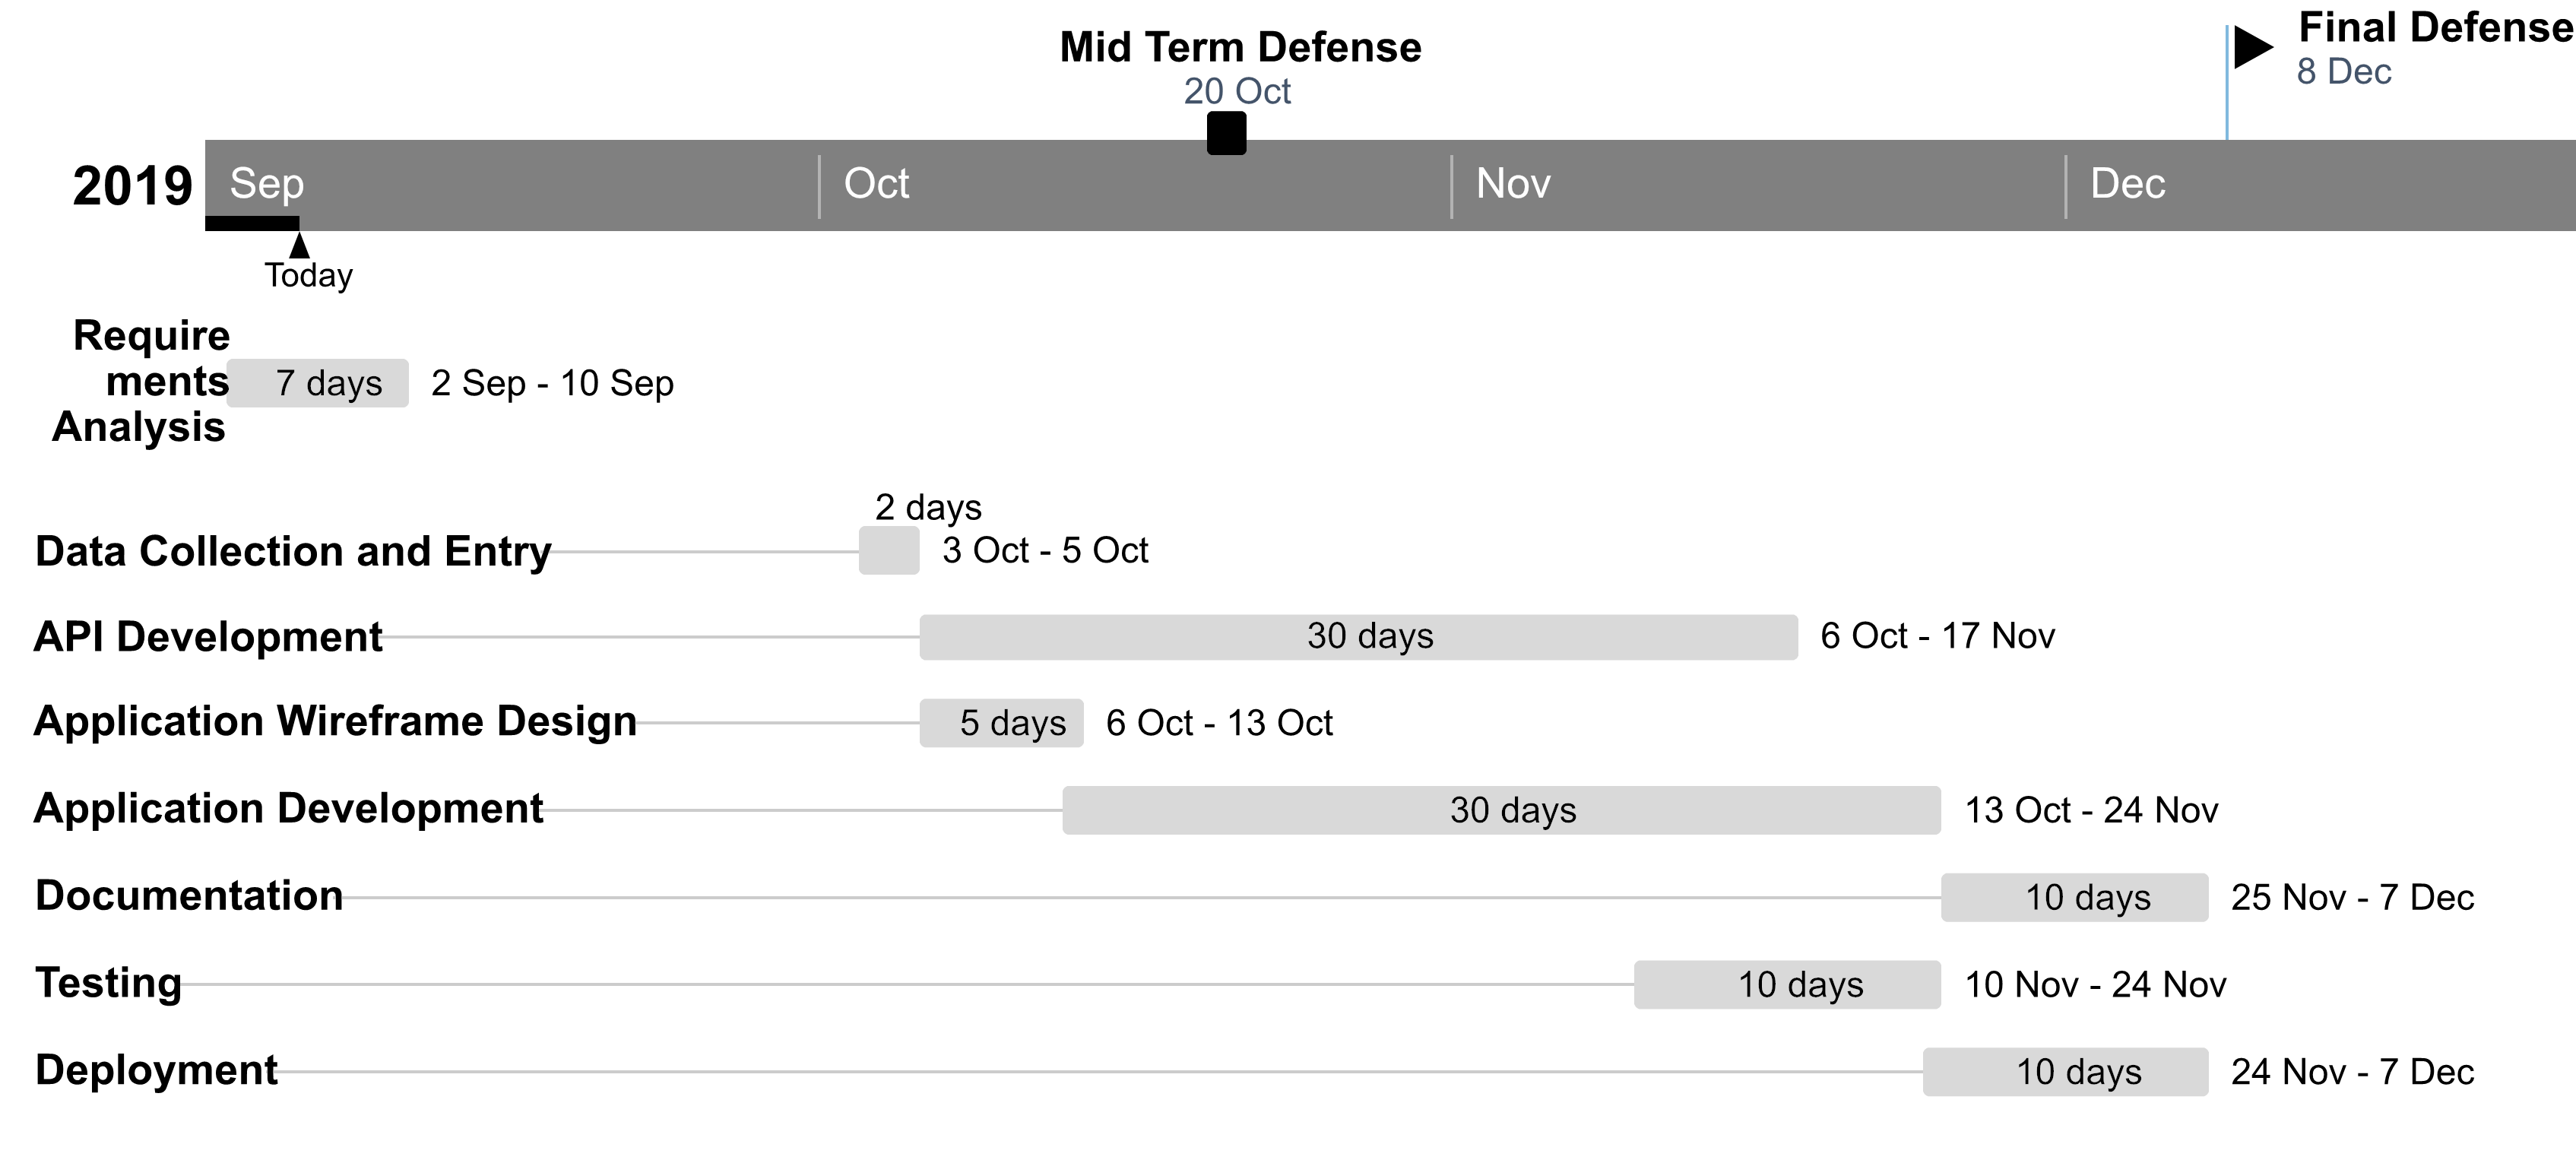
\includegraphics[width=\linewidth]{schedule}
	\centering
	\caption{Project schedule}
	\label{fig:schedule}
\end{figure}

The Proposal Defense of the project was given in 3rd September 2019. The team members worked for a total of around two and a half month on the project. The coding and implementation phase for the backend and front end part were conducted in parallel, which shortened the time taken to complete our project.


\pagebreak
\section{Conclusion}
At the end of the project, a working version of the application Treasure Nepal has been created. The application is in beta phase now, and will soon be released in its stable version.

This project was an endeavor taken by the project team members to contribute in some way to development of tourism in Nepal, and the attraction of tourists to new and unnoticed places in Nepal. The team members firmly believe that the work they have done will certainly be helpful for the Government of Nepal to evenly distribute the tourists in different places in the upcoming Visit Nepal Year 2020. Right now, we are in the phase where the minimal viable product for expanding the scope and commercially developing the project has been created. This MVP could be used to pitch this project idea to investors, policy-makers and the governmental agencies so that this could be further developed and released to the public.

The team members also learnt a lot about the technical framework they used. React Native was a framework unknown to both of the team members but eventually the team members learnt the principles of it and were able to implement it in the project. On overall, it is our conclusion that the project undertaken was completed successfully.

\pagebreak
\section{Further works and Recommendations}
The deliverable provided at the present scope is a minimal viable product that was developed with limited time, resources and cost structure. In the future, this work can certainly be pushed further by adding new features and ideas. Some of the further works recommended by the team members are:

\begin{itemize}
\item The plugins like forex, hotel reservation, ticket reservation, etc could be added to the application so that the application will not only be a method of entertainment to the users, but also a source of information and a tool handy for every tourists visiting Nepal.
\item The fully fledged application could be released to the Google Play Store and App Store so that the users could freely download and use them.
\item The project has a very feasible business model where the hotels, restaurants, etc. that provide the offer could be charged with a subscription fee for having their businesses appear in the application. Moreover, the local advertisements can be shown in the app, which will also generate monetary value. Installing treasures at the hotels and restaurants themselves will even be a better idea. The points division could be designed in such a way that the business paying more fee will get higher point value to the treasure they host.
\item Once enough data is collected from the application users, the data can be processed to find interesting patterns in the data and can be used for the further modification of the business plan. The data can also be used to develop a recommendation engine that recommends places and treasures to the users based on their preferences
\end{itemize}


\break
\addcontentsline{toc}{section}{References}
\bibliography{references}
\bibliographystyle{ieeetran}

\break
\addcontentsline{toc}{section}{Appendices}


\end{document}

%\break
%\section{Proposed Performance Analysis Methodology}
%The performance analysis of the deliverables will be performed according to the popular Top Down Methodology. The main idea in this method is to analyse and address the higher order performance issues at first, then follow the lead upto the lower levels of details if needed \cite{tdmethod}. This methodology is proposed to be followed because it largely reduces the time and cost of assessing the performance since not every modules and sections of the project need to be analyzed at a deeper level.
%
%The final evaluation of the project will be performed by the project evaluation team designated by the college administration.
